
\graphicspath{{ChapterCortex/images/}}
%% Chapitre I %%
\chapter{Cortex modeling via s-reps}
\label{chapter:cortexModeling}

\section{Introduction}
\label{sec:Introduction}

The cerebral cortex is a highly folded slab of neural tissue 
with compact interconnections that enables sophisticated processing of information.
It plays an important role in memory, attention, perceptual awareness, thought, language, and consciousness.
Progress has been made in understanding the structure and function of the cortex.
\cite{lorente1934studies} proposed that the cortex is formed by small cylinders containing vertical chains of neurons; 
These structures were later called columns, corresponding to groups of local cells running perpendicular to the cortical surface.
This hypothesis was later confirmed with the physiological studies done by \cite{mountcastle1998perceptual}. 

The cortex is a layered sheet with a more or less uniform cellular structure. 
It is composed by the following layers:
\begin{enumerate}
 \item Layer I (molecular layer): apical dendrites of cells and axons; 
 \item Layer II (external granular layer): small granule cells and some larger pyramidal cells;
 \item Layer III (external pyramidal layer): small to medium sized pyramidal neurons;
 \item Layer IV (Internal granular layer): interneurons receiving ascending sensory input and projecting to layers II/III. No pyramidal neurons are found in this layer;
 \item Layer V (Internal pyramidal layer): medium to very large pyramidal neurons; 
 \item Layer VI (Multiform layer): assortment of cell types including pyramidal cells, cells that receive input from layers II, III and V and 
       axons projecting to superficial cortical layers and subcortical regions.
\end{enumerate}
Today the columnar organization is the most widely adopted model to explain the cortical processing of information.

\begin{figure}[htb]
 \centering 
    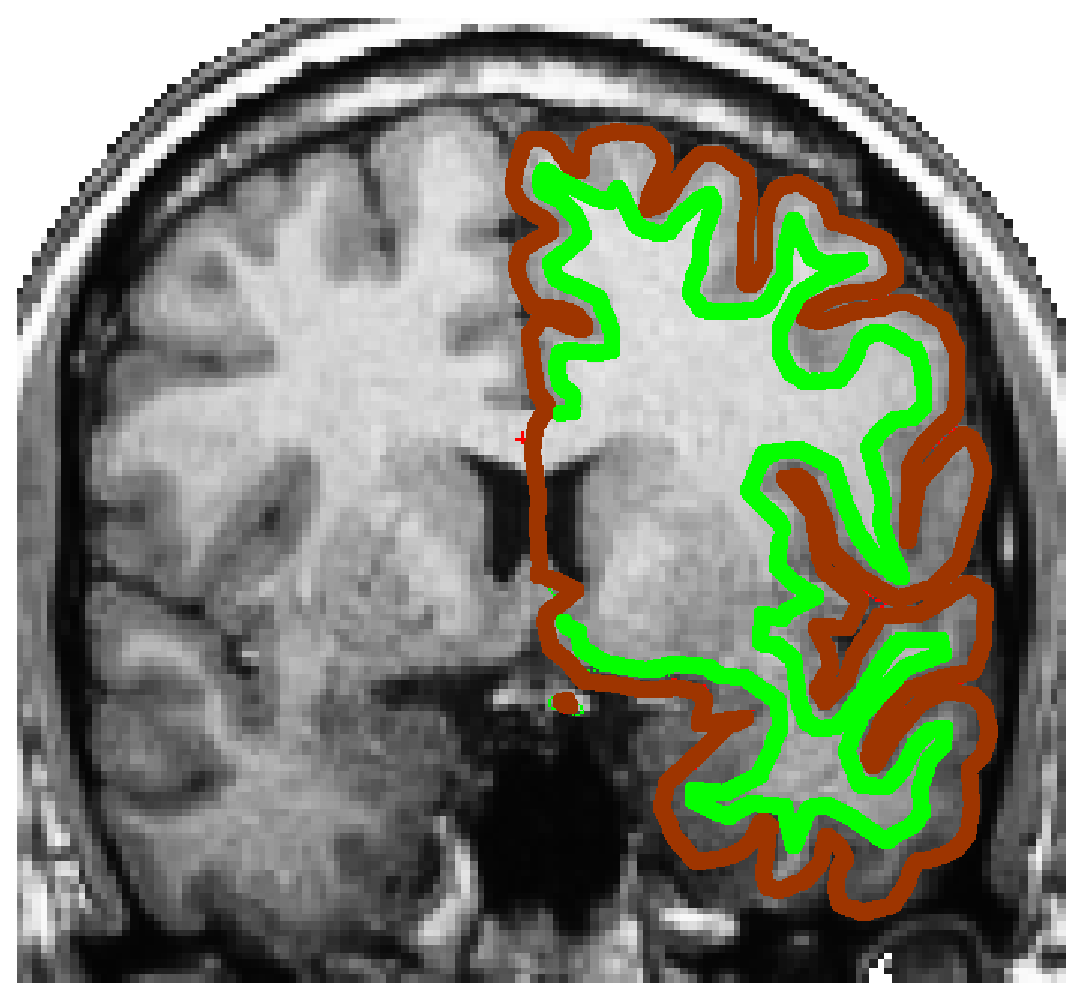
\epsfig{file = lh_BrainFreesurfer.eps, width = 8cm}
 \caption[Brain MRI.]{Brain MRI. The grey and white matter surfaces are shown in brown and green respectively.}
 \label{fig:MRIimage}  
\end{figure}

Figure \ref{fig:MRIimage} shows a slice of an MRI with the cortex region outlined. In brown the grey matter (GM) and in green the white matter (WM) surfaces are shown.
Since nearly two thirds of the cortical surface is buried within the sulci, it is difficult to perform computation and visualization tasks. 
Different procedures have been developed to unfold and map the cortical surface onto different spaces (inflated, spherical or flattened)
\cite{drury_computerized_1996}, \cite{hermosillo_unfolding_1999}, \cite{fischl_cortical_1999}, \cite{pons_area_2004}. 
This allows the cortical surface to be analyzed and visualized and statistical methods to be applied on these spaces.
\textit{Freesurfer} (an automated tool for brain's cortical surface reconstruction using structural MRI data)
uses the inflation and flattening procedure from \cite{fischl_cortical_1999}. 

Likewise, cortex evolution has also been a subject of great interest.
Much of the efforts have been focused on understanding how the folding process occurs.
Many species have folded cortices, but the degree of folding is different among them.
In general terms, a greater degree of folding is related to higher intelligence \cite{buettner1964evolutionary}.
Humans have extremely folded cortices.
%how this process occurs is not clearly understood. 
The folding patterns are 
unique to each brain, and abnormal folding is related to 
neurological disorders such as schizophrenia, epilepsy, autism and Down's syndrome.
Different methods have been proposed to explain how the folding occurs: 
growing a 2D curve in a closed space \cite{raghavan1997continuum}; 
growing 2D and 3D truss elements constrained by radially aligned fibers \cite{toro2005morphogenetic}; 
using spherical wavelets on close surfaces \cite{yu2007cortical}; 
using a FEM (finite element method) biomechanical model \cite{geng2009biomechanisms};
combining a mathematical model with biomechanical data \cite{bayly2013mechanical}.
For a recent review on folding theories see \cite{filas2013mechanisms}.

There are research opportunities in developing cortex models. 
As stated by Javier de Felipe \cite{defelipe2012neocortical}, ``it is still necessary
to achieve a better fundamental understanding of what columns
are and how they are used in cortical processes. Accordingly, it
is now important to translate recent technical advances and
new findings in the neurosciences into practical applications for
neuroscientists, clinicians, and for those interested in comparative
anatomy and brain evolution.''

Taking these facts into consideration, one of the objectives in this dissertation is to provide a
tool that models the shape of the cortex and relates to the real physical structure. 
Section \ref{sec:s-repImplementation} defines an s-rep
with the corresponding interpolation mechanisms that parameterize the interior of the object by $[u, v, \tau]$.
S-reps can be used to model the anatomic and physiologic information from the different layers of the cortex.
This information can be naturally included using the $\tau$ coordinate.

\begin{figure} 
 \centering 
	\subfigure[]{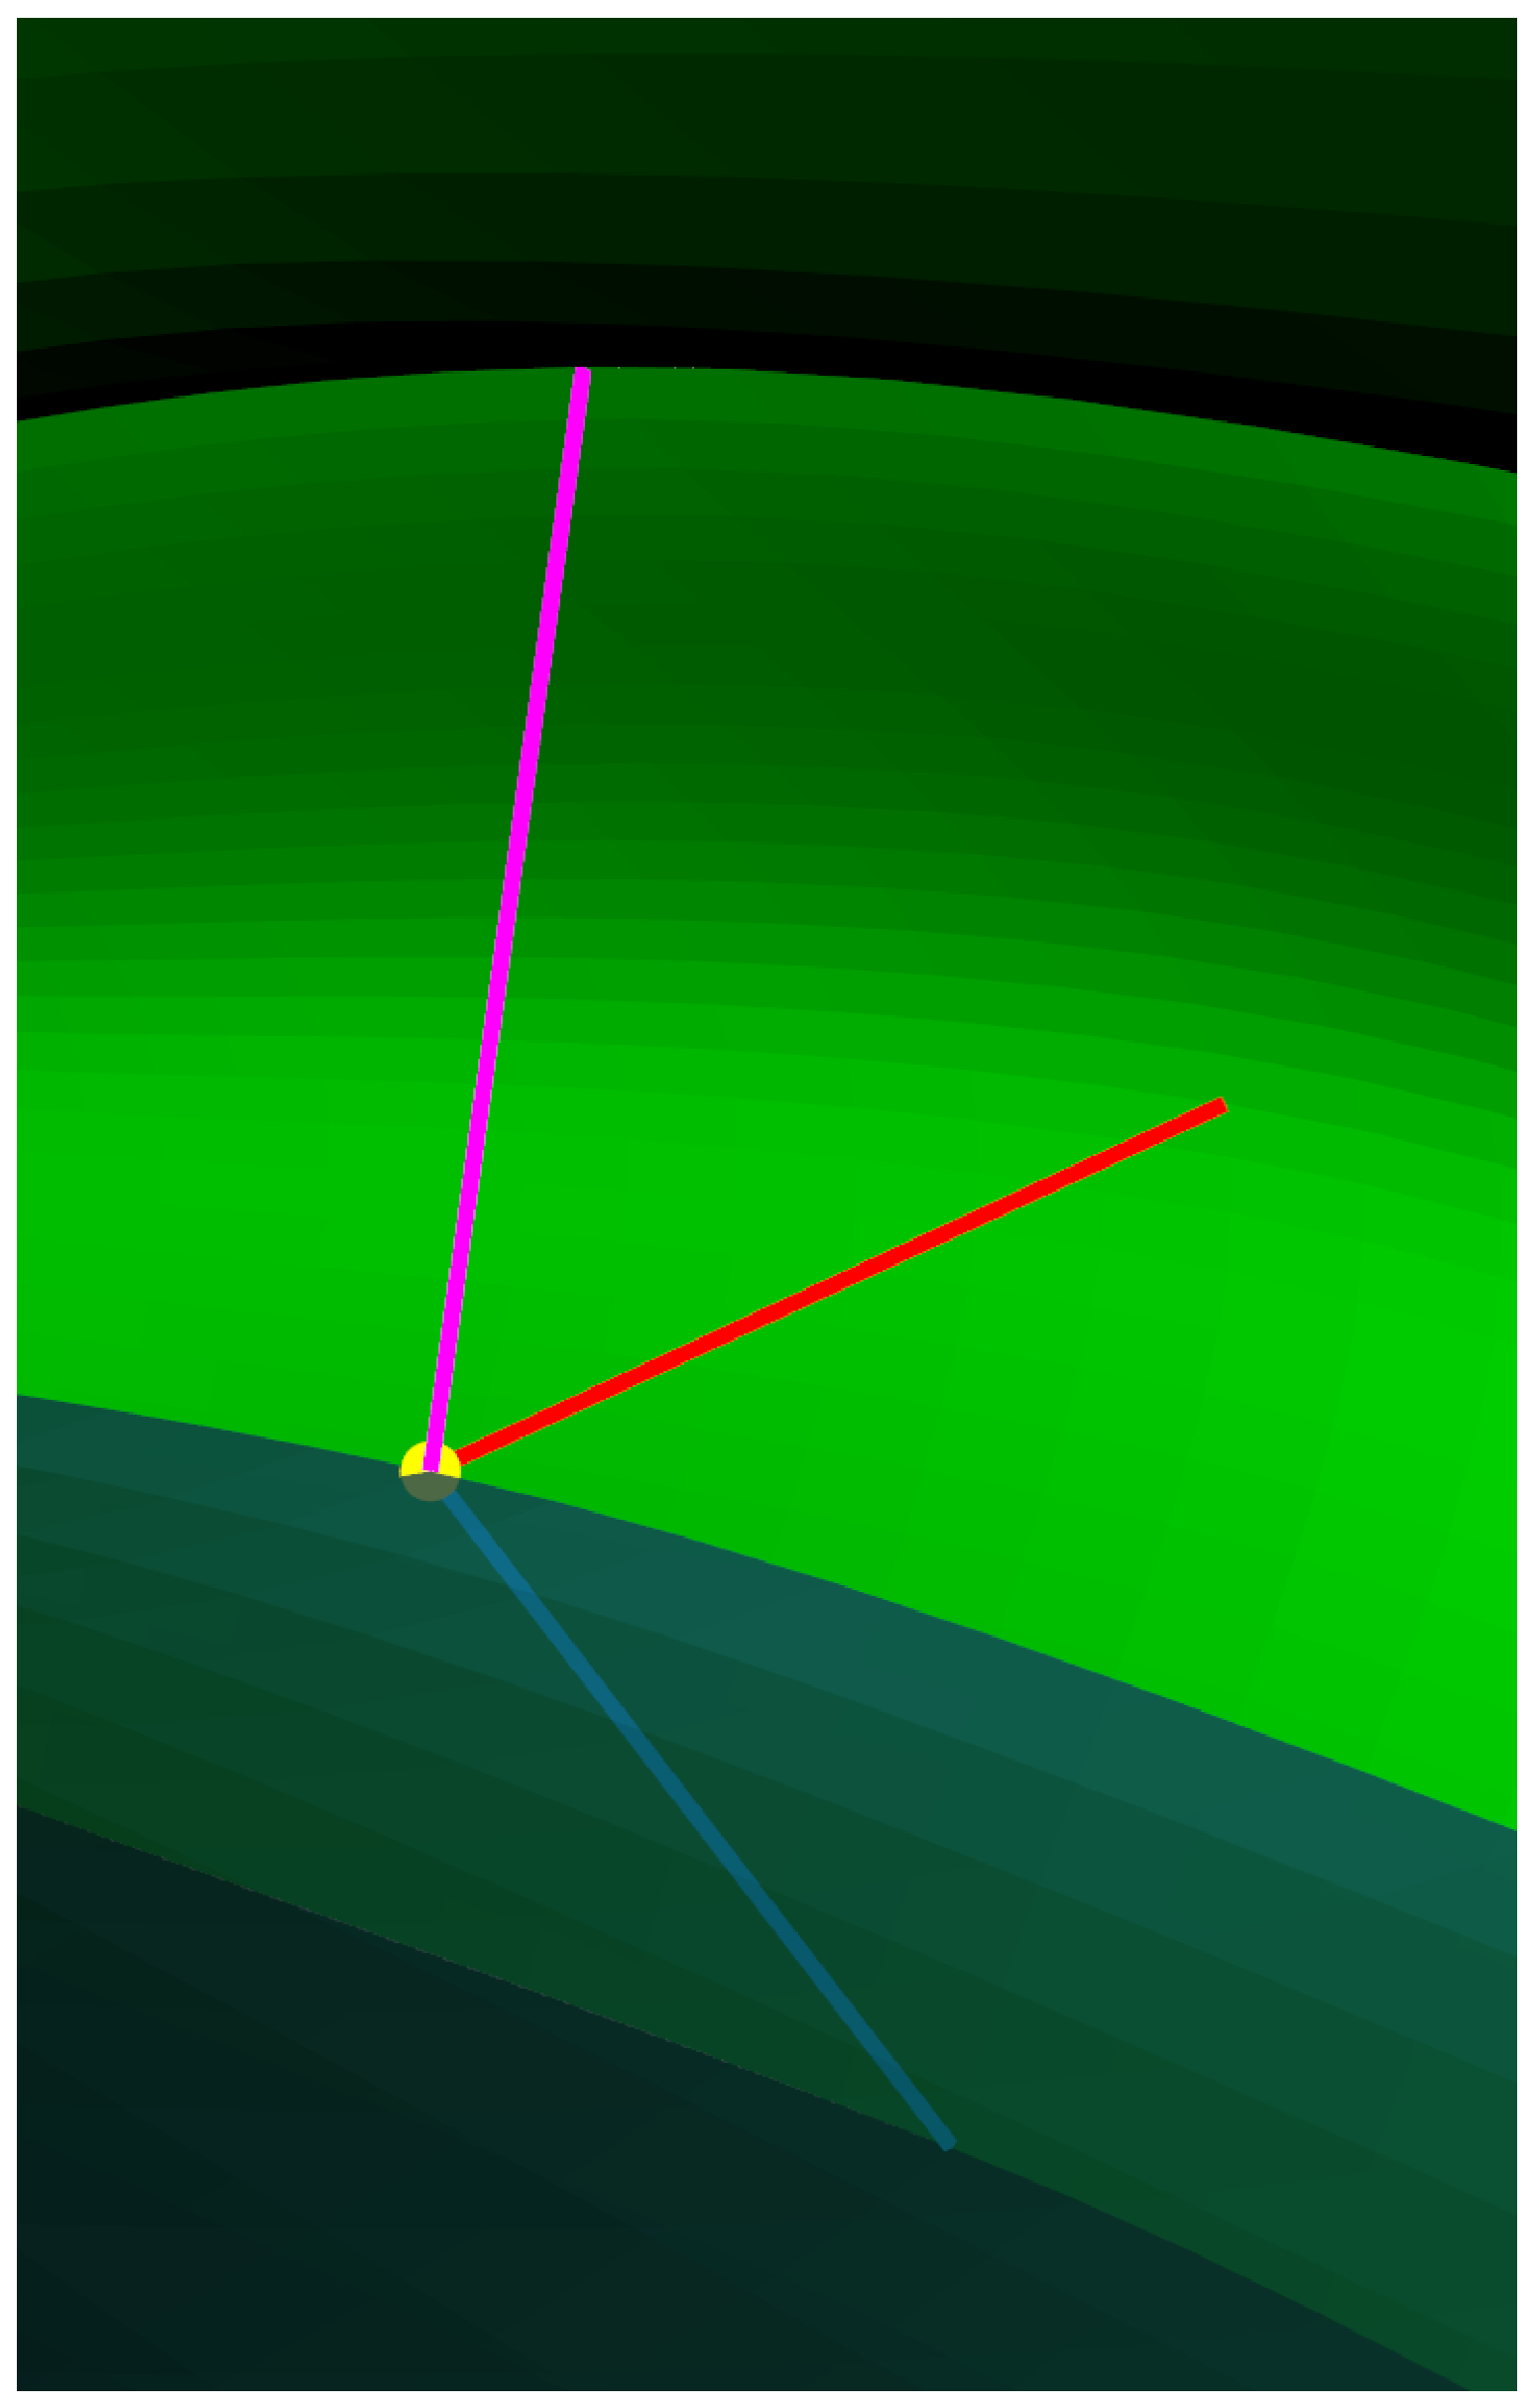
\epsfig{file = s-repatomCloseUp.eps, width = 3.25cm}}
	\subfigure[]{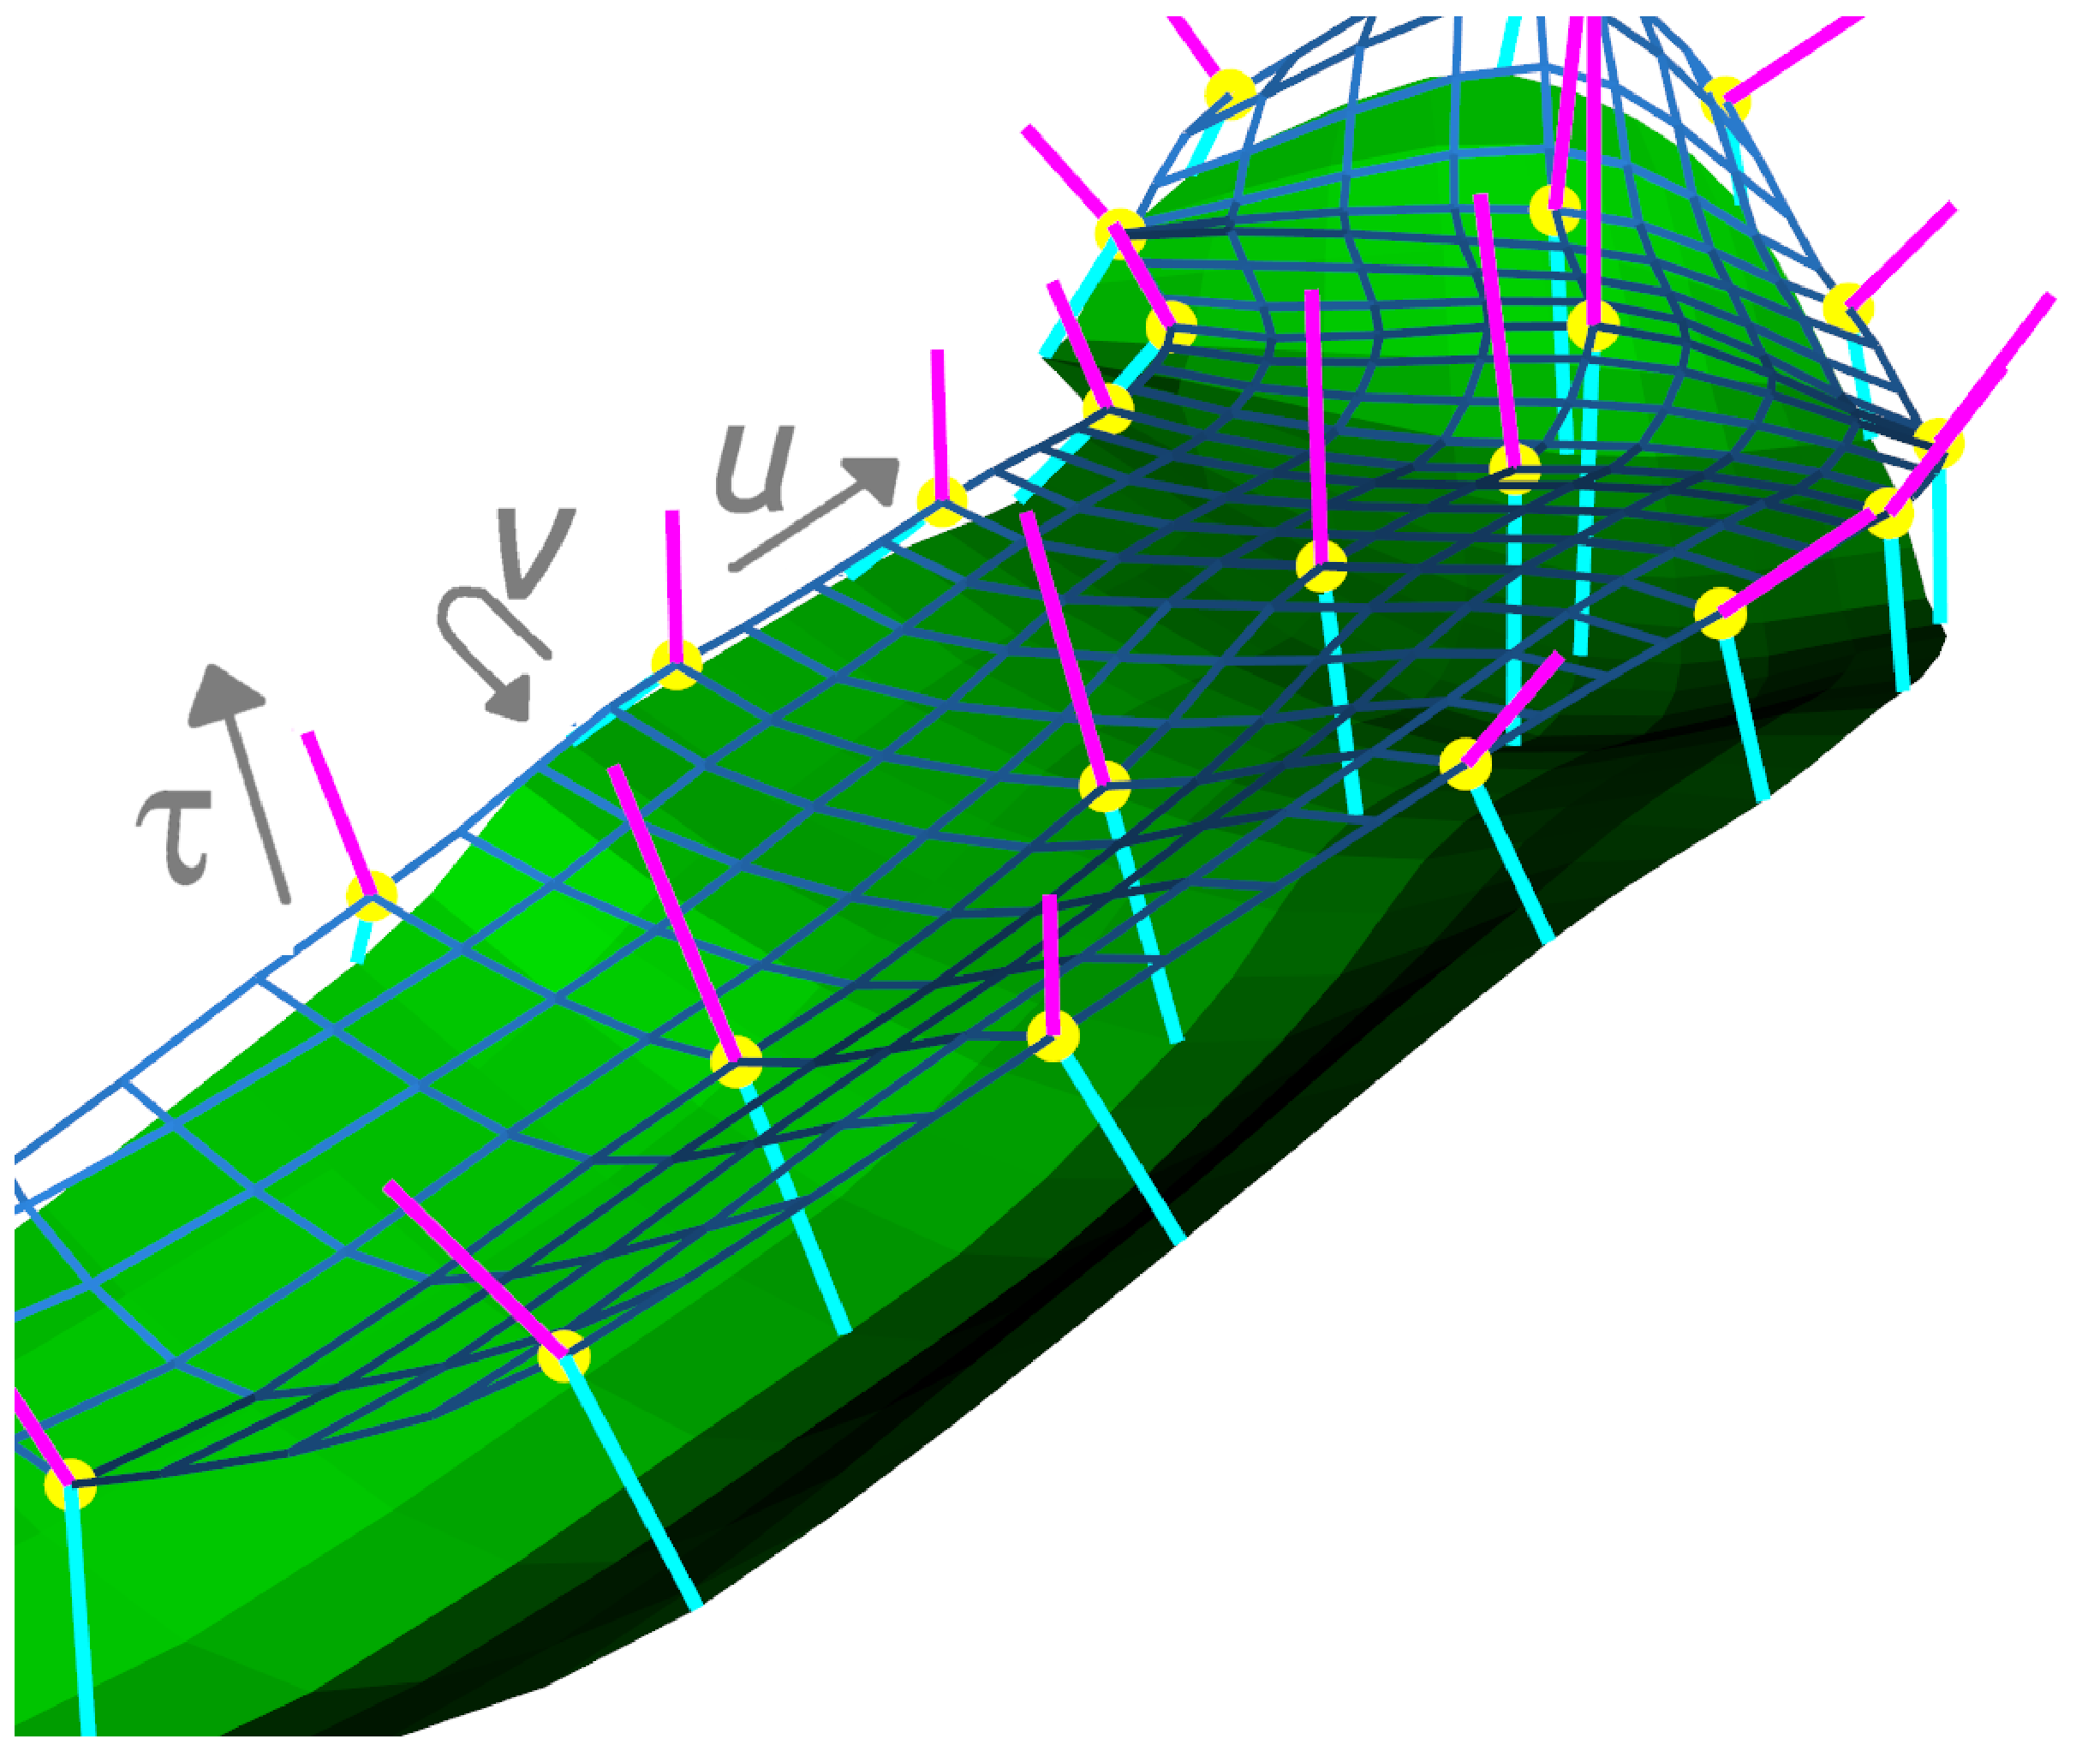
\epsfig{file = s-repFig.eps, width = 6cm}}
	\subfigure[]{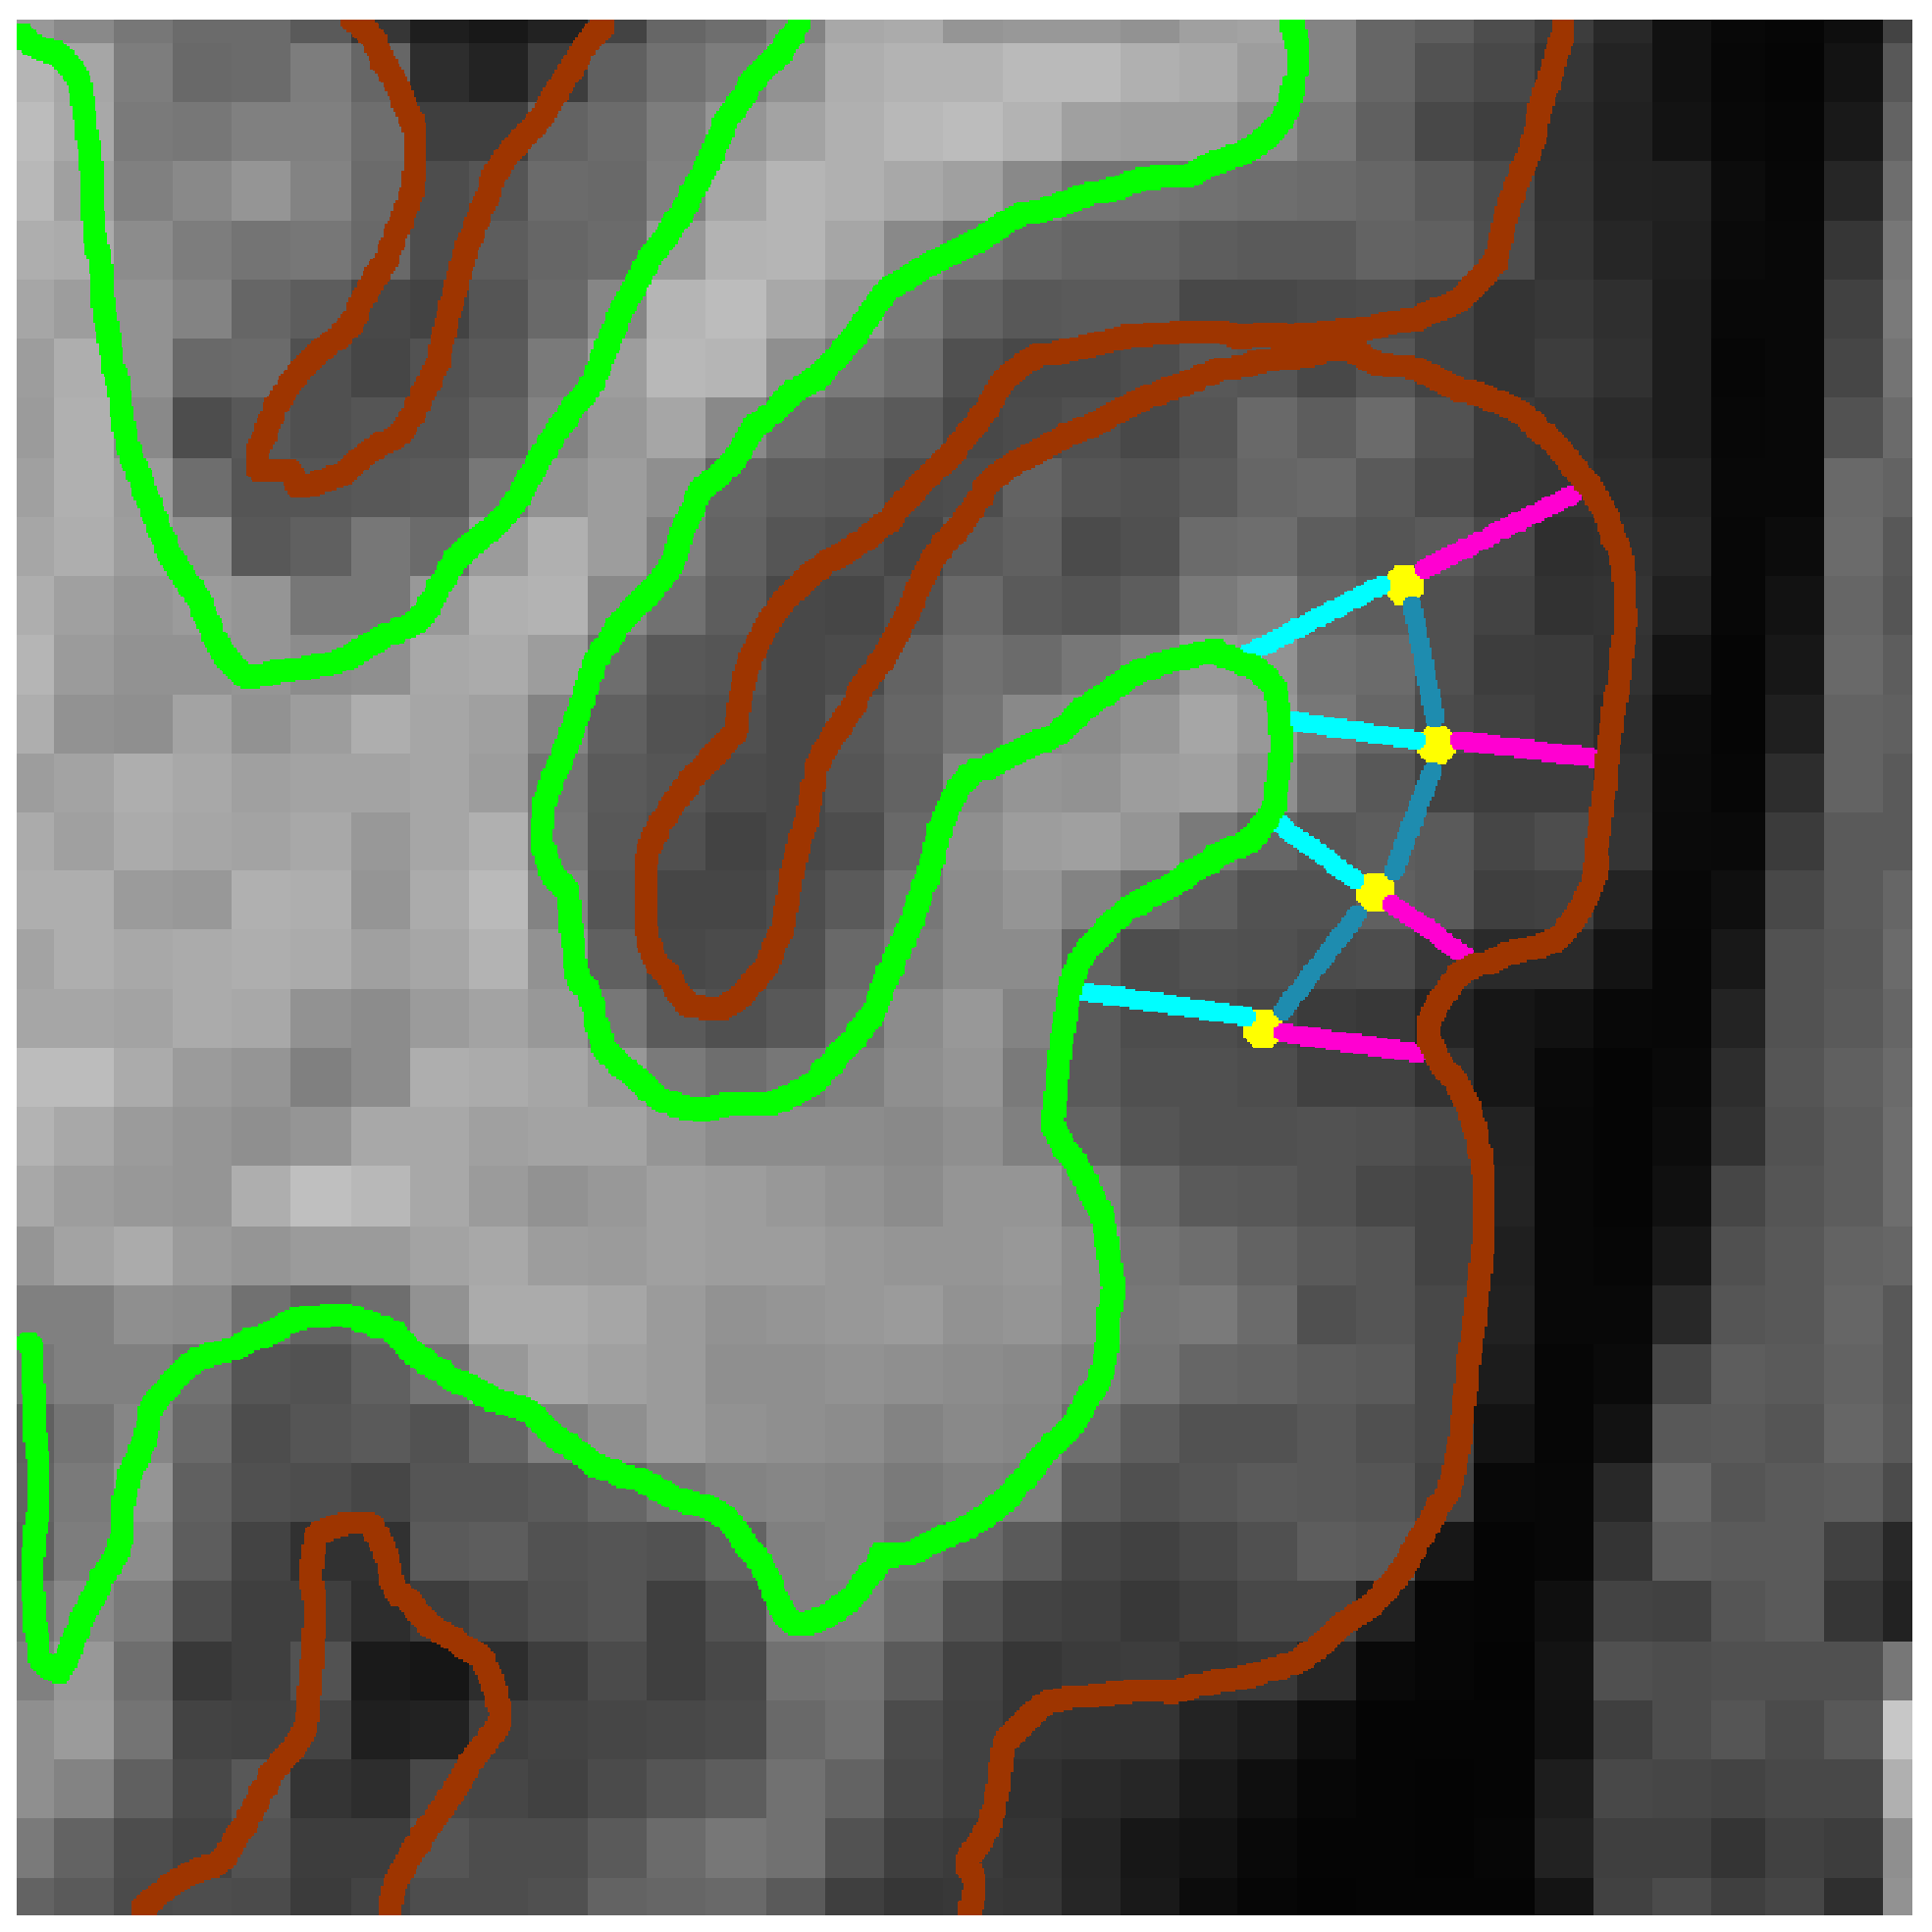
\epsfig{file = lh_BrainFreesurferZoom.eps, width = 5cm}}
 \caption[Atom close up.]{Figure (a) shows a close up of an atom represented as the yellow ball with its corresponding spokes, top (magenta), bottom (cyan), crest (red). 
          The s-rep on figure (b) shows the quasi-medial surface in wireframe representation (blue), with the sampled atoms.
          The MRI image on figure (c) shows a cross-section of the skeletal locus of the cortex and some atoms with the corresponding top and bottom spokes.}
 \label{fig:srepfigCortex}  
\end{figure}

%S-reps are defined as continuous objects using the interpolation mechanisms described in \cite{pizer_nested_2012},
%meaning that every point inside the object has a unique set of coordinates $[u, v, \tau]$. $u$ codes the width, $v$ the length of the medial locus,
%and $\tau$ the thickness of the object.
%$u$ varies from 0 to 1, $v$ wraps around the object with $v < 0.5$ on the ``anterior'' and $v > 0.5$ on the ``posterior'', and $\tau$ 
%from the skeletal locus to the object boundary, as shown in Figure \ref{fig:Srepfig}-b.
%The union of vectors form the object boundary and the union of tails represent the ``skeletal locus''. 
%Notice that s-reps model the continuum space, opening the possibility to include the cellular level and describe the layered structure 
%of the cortex.
Figure \ref{fig:srepfigCortex} shows how an s-rep fits into the cortex. 
%From now on the word s-rep is used to reference the discrete version of the object.

Besides shape description, s-reps have been used successfully to compute shape statistics and mean shapes from a population 
of objects. 
%This is done using CPNS a method analogous to PCA \cite{pizer_nested_2012}.
With this statistical description, it appears to be possible to classify objects by shape frequently more accurately than any other method.
%The majority only use surface information; in contrast, the skeletal structure brings 
%stability to the statistics and increases the correspondence of information across the population of objects.
%S-reps have been used to model internal brain structures such as the hippocampus \cite{pizer_nested_2012}. 
S-reps model single non-branching objects, and tubular objects, as explained in Section \ref{sec:quasiMedial}.
The objects modeled with s-reps until now are simple as most of them have a 
blob-like or elongated shape structure like the the hippocampus \cite{pizer_nested_2012}.

It is demonstrated that s-reps are suited to represent a folded complex structure such as the cortex.
The sheet of the object does not branch and captures the majority of the folds in the cortex. 
Moreover, a statistical analysis of shape variability is done using the s-rep description of the cortex.

The following section explains how to create an s-rep of the cortex from an MRI image.
The procedure uses a spherical representation of the cortex  \cite{fischl_cortical_1999} 
that relates the WM and the GM surfaces to the sphere.
Folding the s-rep into the cortex is done by 
projecting the SS (skeletal sheet) of the s-rep on the sphere and 
using the relationship of the sphere and the cortical surfaces.
%The folding procedure uses a function 
%that minimizes the distance to a set of closest points in the WM and GM surfaces.
%The procedure is done for every atom. It maintains
%the topology and regularity of the quads 
%or quadrangles that form the SS of the s-rep (quad definition in Equation \ref{equ:Quad}).
The following section explains in detail the procedure to create an s-rep of the cortex.
With the skeletal figure inside the cortex, 
top and bottom spokes point towards the GM and WM surfaces respectively.
The interpolation mechanisms of the s-rep allows reconstructing the GM surface and the WM surface.
Section \ref{sec:Evaluation} evaluates the quality of the interpolated surfaces.
Finally, a population of cortex s-reps is generated, and a statistical analysis is made in Section \ref{sec:Statistics} using CPNS (Composite Principal Nested Spheres, which is  
described in Appendix \ref{sec:apendixCPNS}).

\section{Acknowledging the true shape of the cortex}
\label{sec:s-repFittingCortex}


\begin{figure*} 
 \centering 
	\epsfig{file = DiagramProy.eps, width = 15cm}
 \caption[Flow diagram of s-rep projection and cortex folding.]{(a) Inflation of the cortex by \textit{Freesurfer} and rotation of the sphere to the north using the points in the corpus callosum. 
          (b) Transformation of a base s-rep into a circle.
          (c) Transformation of the circle into a sphere. 
          (d) Fitting the s-rep to \textit{Freesurfer's} data on the sphere.
          (e) Folding the SS of the s-rep inside the the cortex and determine the widths of the slab. 
          }
 \label{fig:proyProcedure}  
\end{figure*}

The cortex is a highly folded sheet. It has thickness that varies through the cortical regions. 
Unfortunately, the cortex is often represented using surfaces and is difficult to 
represent interior  features.
To acknowledge its true shape which is similar to a folded pancake, 
a procedure to create an s-rep of the cortex is proposed. 
As shown in Figure \ref{fig:proyProcedure}, the procedure has five steps:

\begin{enumerate}[(a)]
 \item A mapping of the cortex on a sphere is done using the method from \cite{fischl_cortical_1999}. 
       The sphere is rotated to the north using the corpus callosum.
 \item A regular grid or the SS of a base s-rep is transformed into a 'circular log-grid'.
 \item The 'circular log-grid' is transformed into a sphere (with a spherical cap oppening in the north pole).
 \item The SS on the sphere is fitted to the mapping of the cortex on the sphere.
 \item The SS is folded back into the shape of the cortex. During the folding procedure, the widths of the slab or the thickness of the s-rep is determined.        
\end{enumerate}

The following sections explain the details of each step and shows how to create an s-rep 
of the cortex.


\subsection{Spherical representation of the cortex by \textit{Freesurfer} and rotation}
\label{sec:Materials}

The materials used in this study are 8 
MRI scans acquired at ``CERMEP - Imagerie du vivant'' 
%********************* 
on a Siemens 
Sonata system with a 1.5 T magnet, with gradients of 40 mT/m and an 8-channel head coil. 
The overall protocol includes anatomical acquisitions, spectroscopy and diffusion.

In this study, only T1-weighted anatomical images are considered. The 8 datasets were obtained by
the acquisition of millimetric sagittal slices from a 3D T1-weighted MPR sequence (repetition time (TR) = 1880 ms, echo time (TE)
Ms = 4).
The total acquisition time of each of these anatomical images was done in 18 minutes.

All the datasets were segmented using \textit{Freesurfer}.
%and the inflation and flattening procedure from \cite{fischl_cortical_1999}.
The method proposed by \cite{fischl_cortical_1999} 
creates a spherical representation of the cortex. It removes the folds from the surface using an energy functional 
with a distance term for unfolded or positive regions. 
An unfolded region is recognized by calculating the normal direction and the ordered cross-product
of the triangle legs for every face in the surface tessellation. If the resulting vector 
is anti-parallel to the normal direction, a negative area is assigned. 
The folds from the surface are eliminated when the area is constrained to be
positive everywhere.
After the inflation procedure, the cortical surface has spherical topology. 
A mapping of the cortex is made onto a sphere providing 
a $1-1$ relationship for every point on the cortical surface and spherical mapping.
%The spherical mapping is the key to construct the s-rep of the cortex. 

The procedure to build the s-rep of the cortex uses a modified stereographic projection.
The stereographic projection \cite{snyder_map_1987} was probably known to the Egyptians in its polar form, 
but Hipparchus (2nd Century B.C) was apparently the first Greek to use it, so he is considered its inventor. 
Ptolemy referred to it as ``Planisphaerum'', the name stereographic was given by Fran\c{c}ois d'Aiguillon in 1613.
The stereographic projection enables a mapping of the points on a plane
to the sphere and it has two properties that should be treated carefully:
%is conformal (preserves angles), azimuthal (all points are proportionally correct distances from the center point),
the scale increases away from the center of the projection,
and the point opposite to the center of the projection cannot be plotted (north pole).

The first step to do a stereographic projection is to choose the north pole. 
The north pole of the sphere cannot be mapped by the stereographic projection because it
maps to infinity. For this reason, the representation must have a spherical cap opening in the north pole.

The corpus callosum is a brain structure located 
beneath the cortex. It facilitates inter-hemispheric communication with a bundle of 200-250 million fibers for this task.
Figure \ref{fig:Corpuscallosum} displays the corpus callosum. 
This brain structure is used to find the north pole.
The points in the corpus callosum are used in a fitting procedure that minimizes the geodesic distance from each point to a circle. 
The center of the best fitting circle is chosen to be the north pole.
%The point opposite to the north pole is the center of projection.

\begin{figure} 
 \centering 
 \subfigure[The internal part of the left hemisphere of the cortex. 
            The corpus callosum is shown in the figure.
            The points that compose the corpus callosum are used in the minimization procedure.]{\epsfig{file = corpuscallosum.eps, width = 7.25cm}}
 \subfigure[Spherical representation of the left hemisphere. 
            The best fitting circle is shown in cyan and the projected points  
            on top of the circle in magenta. The center of the circle is aligned with the north pole.]{\epsfig{file = sphereRotationNorth.eps, width = 7.25cm}}
 \caption[Inflation procedure, mapping the cortex on a sphere.]{The inflation procedure maps the cortical surface onto a sphere. 
          The best fitting circle is found using the points of the corpus callosum.}
 \label{fig:Corpuscallosum}  
\end{figure}

To find the best circle for a set of points in a sphere, a method similar to \cite{jung_analysis_2012} is used.
A circle on the sphere $S^2$ is defined by a vector $v_1$ and a distance $r_1 \in (0, \pi/2]$ as in equation \ref{equ:circle0},
where $\rho_d$ is the geodesic distance function.

\begin{equation}  
	C(v_1, r_1) = \{x \in S^2 : \rho_d(v_1, x) = r_1\}.
  \label{equ:circle0}
\end{equation}
The best fitting circle is found with a least squares minimization
that uses the geodesic distance as follows:
let $CC = \{x_i: i \in N\} \in S^2$ be the points of the corpus callosum on the sphere. We first define the residual $\varepsilon$ of $x_i$ from a circle
$C( v_1 , r_1 )$ of $S^2$ as the signed length of the minimal geodesic that joins $x_i$ to $C$. Then 
$\varepsilon = \rho_d( v_1 , x ) - r_1$. The sign of $\varepsilon$ is negative if $x_i$ is in the interior of $C$, and is positive if $x_i$ is in the exterior.
The best fitting circle $\hat{C} \equiv C( \hat{v}_1 , \hat{r}_1 )$ 
is found by minimizing the sum of squares of residuals of the data points to $C$. 
In other words $v_1$ and $r_1$ minimize Equation \ref{equ:optimalcircle}.

\begin{equation}  
  \hat{C} = \operatorname*{Arg\,min}_{v_1, r_1} \sum_{i=1}^{n} \varepsilon_i ( v_1 , r_1 )^2 = \operatorname*{Arg\,min}_{v_1, r_1} \sum_{i=1}^{n}\{\rho_d(x_i, v_1) - r_1 \}^2
  \label{equ:optimalcircle}
\end{equation}

Once the center of the circle is found, 
a rotation is done to align its center to the north pole. 
%A second rotation is performed to align it with the x axis. 
%This is done by finding the average point on the circle for the projected data, calculating the tangent at this point,
%and computing the opening angle with the x axis.
Figure \ref{fig:Corpuscallosum} shows the corpus callosum and a spherical representation 
of the cortex with the best fitting circle. 

The following section explains how to modify the s-rep 
to produce the best possible mapping on the sphere. 
The projection to the sphere is explained in Section \ref{sec:StereographicProjection}.

\subsection{Transforming the s-rep into a circular log grid}

An s-rep is built using a grid of sampled points where
each intersection is a hub or atom of the s-rep. 
An atom is defined as a sampled point on the SS or quasi-medial surface of the object as shown in Figure \ref{fig:srepfigCortex}-a.

To generate the s-rep of the cortex, the structured collection of atoms (the grid) is mapped on a sphere.
This mapping is equivalent to the mapmakers problem, \textit{i.e.}, to map two surfaces with
different Gaussian curvatures. This was shown to be impossible by Gauss in 1828.
To lower the distortion effects of the projection and allow the construction of the s-rep, 
the grid of the s-rep is modified.
This is done to improve the sampling of the hubs on the sphere while preserving the grid topology.

Relating the points from the plane to the sphere is the key to produce the s-rep of the cortex. 
Each projected hub can be related to the spherical representation of the cortex provided by \textit{Freesurfer}.
%(an automated tool for brain's cortical surface reconstruction using structural MRI data).

\begin{figure}[h!]
 \centering 
 \subfigure[Regular grid]{\epsfig{file = regularGrid.eps, width = 4.5cm}}
 \subfigure[Log grid]{\epsfig{file = logGrid.eps, width = 4.5cm}}
 \subfigure[Circular log grid]{\epsfig{file = logGridCircular.eps, width = 4.5cm}}
 \caption[Resampling of the s-rep.]{An s-rep is represented with a grid of points. If the regular grid is projected on the sphere
          a distortion effect is produced by the stereographic projection. In order to lower the distortion effects, the grid is resampled
          using a log function. The transformation into a circle is done to match the s-rep to the best-fitting circle of the corpuscallosum.}
 \label{fig:gridTransformation}  
\end{figure}

An s-rep is represented by a regular grid on a plane.
Mapping a regular grid on the sphere 
causes a distortion since 
the majority of the hubs will map towards the north pole (first property of the stereographic projection).
To produce the best s-rep of the cortex and capture accurately the geometry of the folds,
the hubs should be spaced evenly on the sphere. 

To attain a regular spacing of the hubs, a log function is used to resample the position of the hubs in the grid. 
Figure \ref{fig:gridTransformation} shows how the log function maps more points towards the center of projection.

\begin{equation}
  S(x) =  \left\{
		  \begin{array}{lr}
			  Min + x*(\frac{Max - Min}{N/2}), & x < \frac{N}{2} \\
			  Min + (N-x)*(\frac{Max - Min}{N/2}), & otherwise
		  \end{array}
  \right.  
  \label{equ:step}
\end{equation}

\begin{equation} 
 L(S(x)) = \left\{\begin{array}{lr}
			  \frac{log(S(x))}{log(Min)}, & x < \frac{N}{2} \\
			  -\frac{log(S(x))}{log(Min)}, & otherwise
		  \end{array}
		  \right.
  \label{equ:logscale}
\end{equation}

Equations \ref{equ:step} and \ref{equ:logscale} show how to transform the regular grid.
Each hub $(x,y) \in [0, N-1]$ is distributed regularly with $S(x) \in [Min, Max]$
where $N$ is the number of points for one side of the grid,
$Min \in (0, Max)$, and $Max$ is always set to 1.
$L(S(x)) \in [-1, 1]$ moves the points towards the center 
of projection (south pole). Having an increased number of 
points near the center reduces the distortion effects 
produced by the stereographic projection.

Finally, to further improve the projection of the grid on the sphere, 
the grid is transformed
into a circle as described in \cite{nowell_philip_math}.
By projecting the circle on the sphere, the spherical cap opening
required by the stereographic projections is naturally found.
Equation \ref{equ:squaretocircle} shows how the transformation is done. 
Notice that the points over the axis do not change, points in the corners get normalized and all others are 
transformed accordingly, as shown in Figure \ref{fig:gridTransformation}.
%for an example on the effect of 
%different grid types on the final cortex representation, see Figure \ref{fig:BestCircle}.

\begin{equation}  
	\begin{array}{lcr}
		x' & = & x \sqrt{1 - \frac{1 - y^2}{2}} \\
		y' & = & y \sqrt{1 - \frac{1 - x^2}{2}} 
	\end{array}  
  \label{equ:squaretocircle}
\end{equation}

%\begin{figure} 
%\vspace{-0.2cm}
% \centering 
% \subfigure[Square log grid]{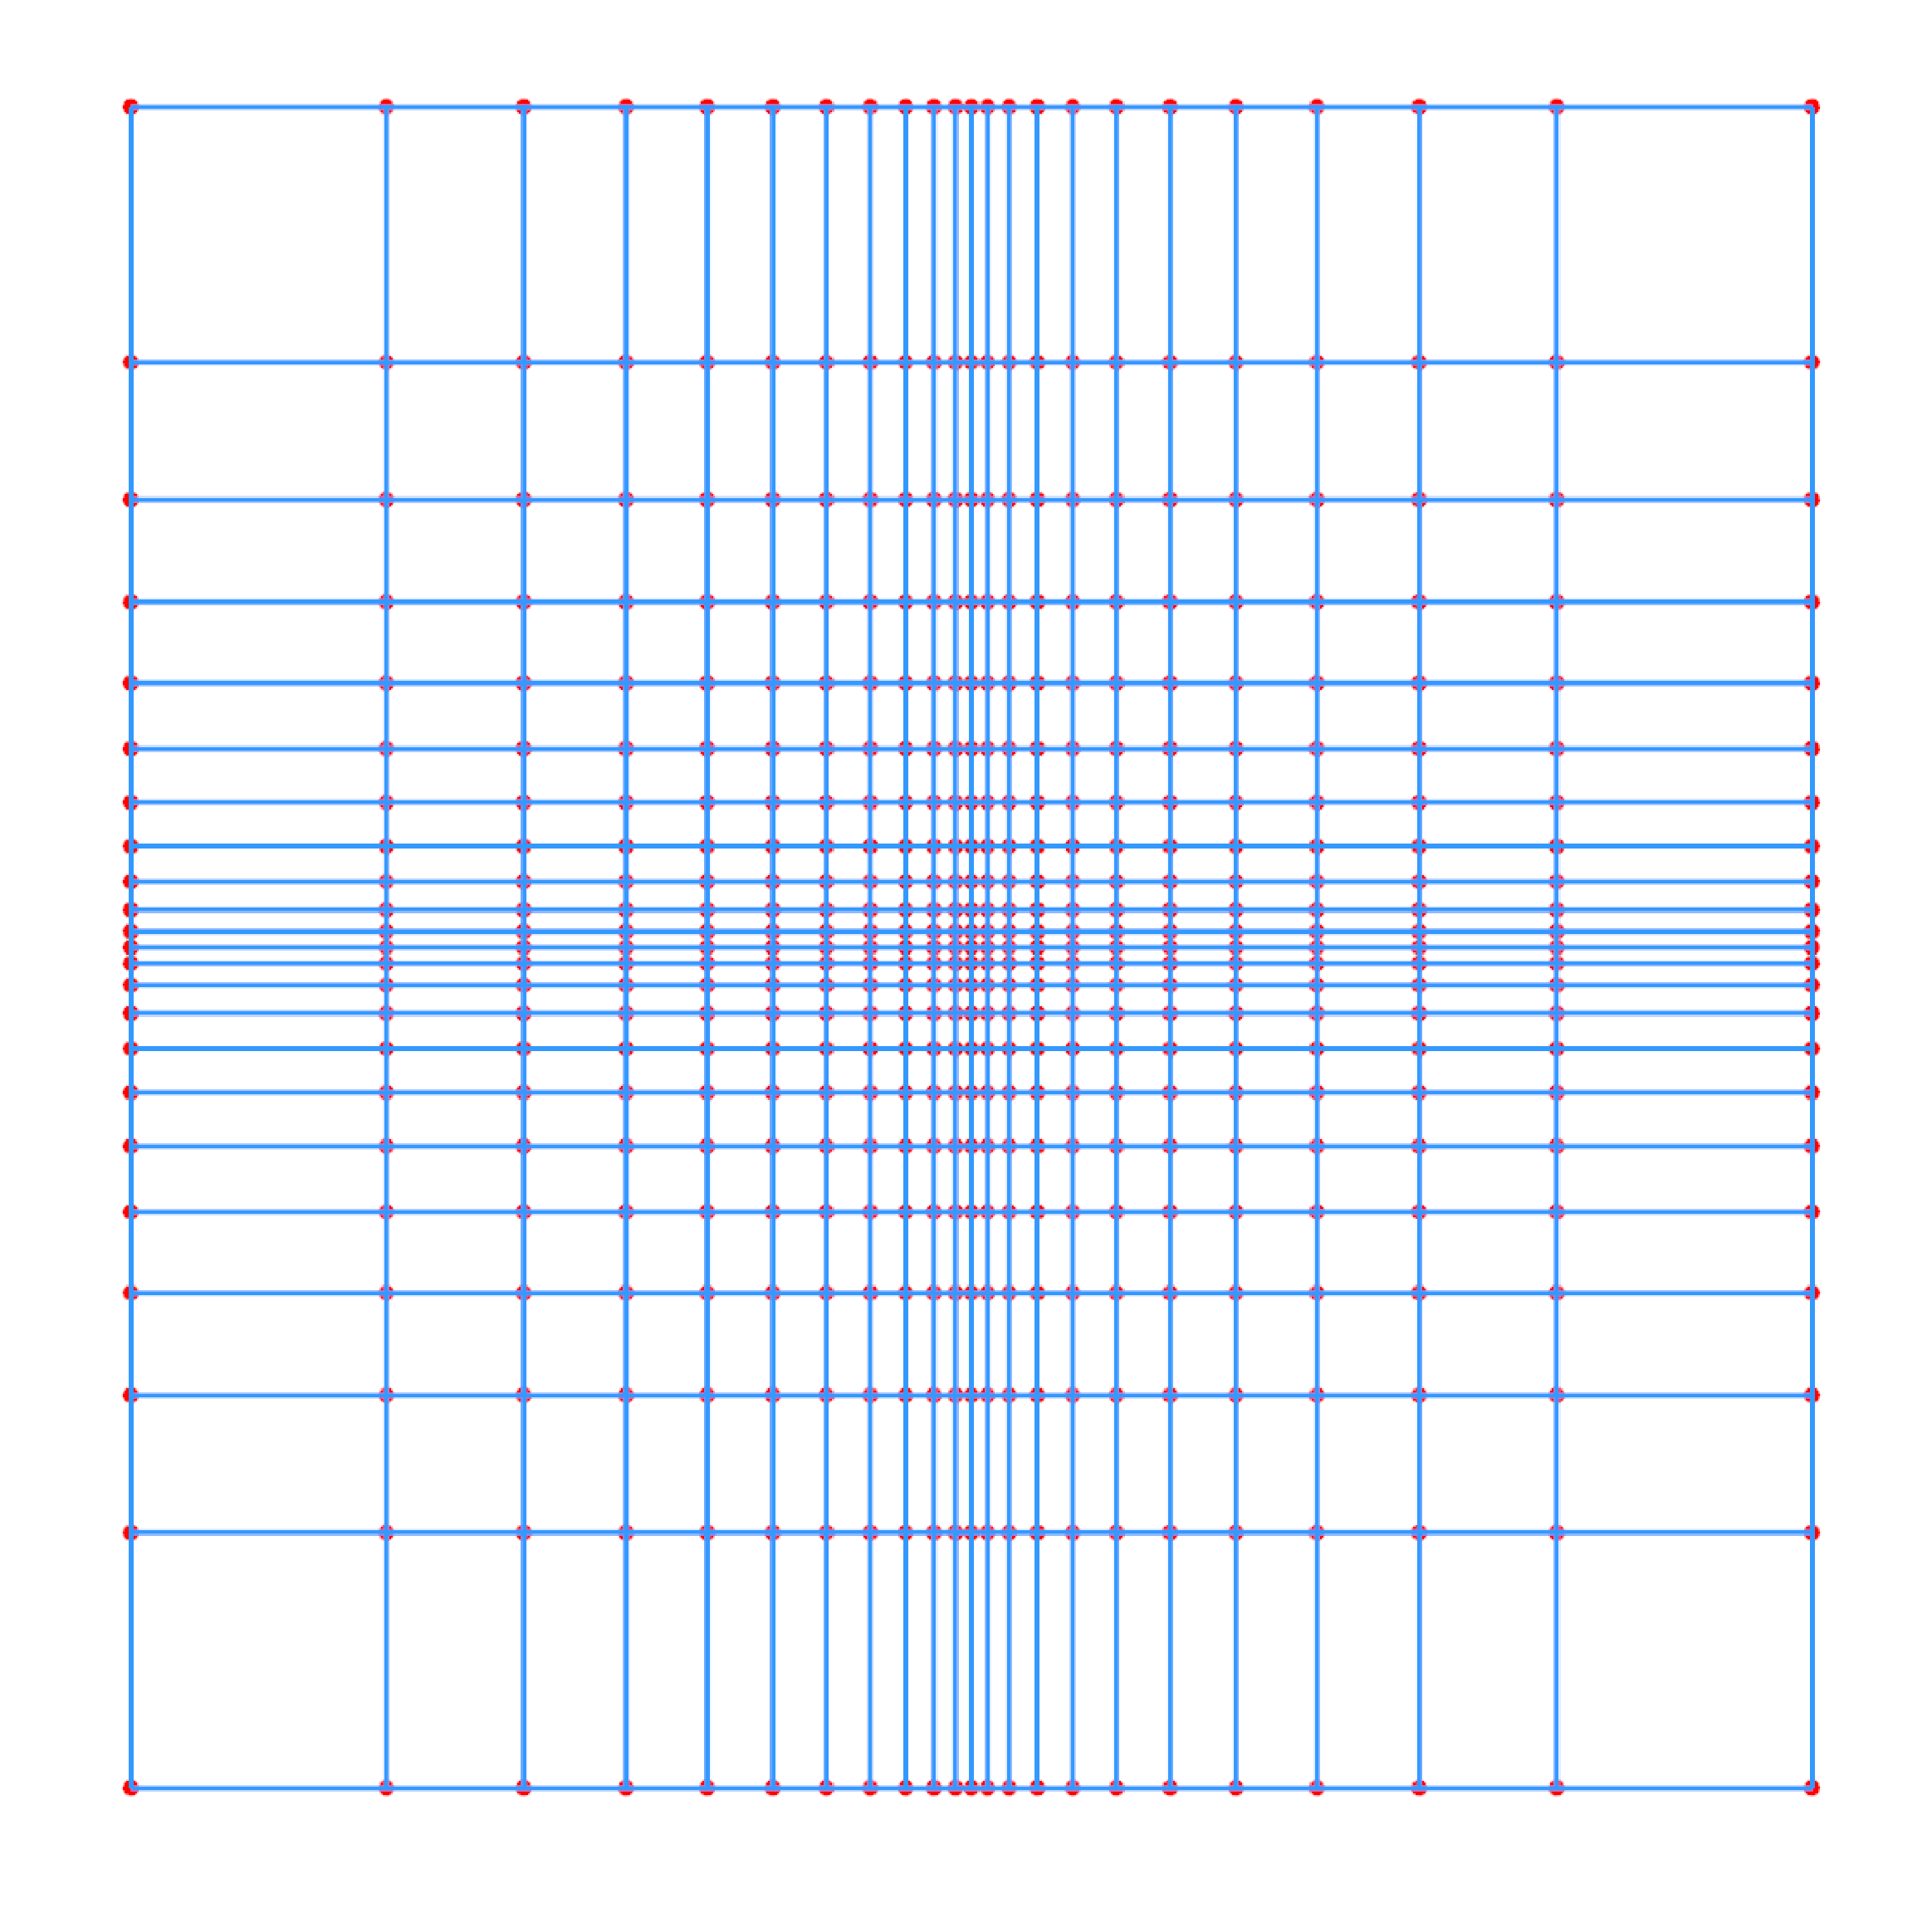
\epsfig{file = square_s-rep.eps, width = 3cm}}
% \subfigure[Circular log grid]{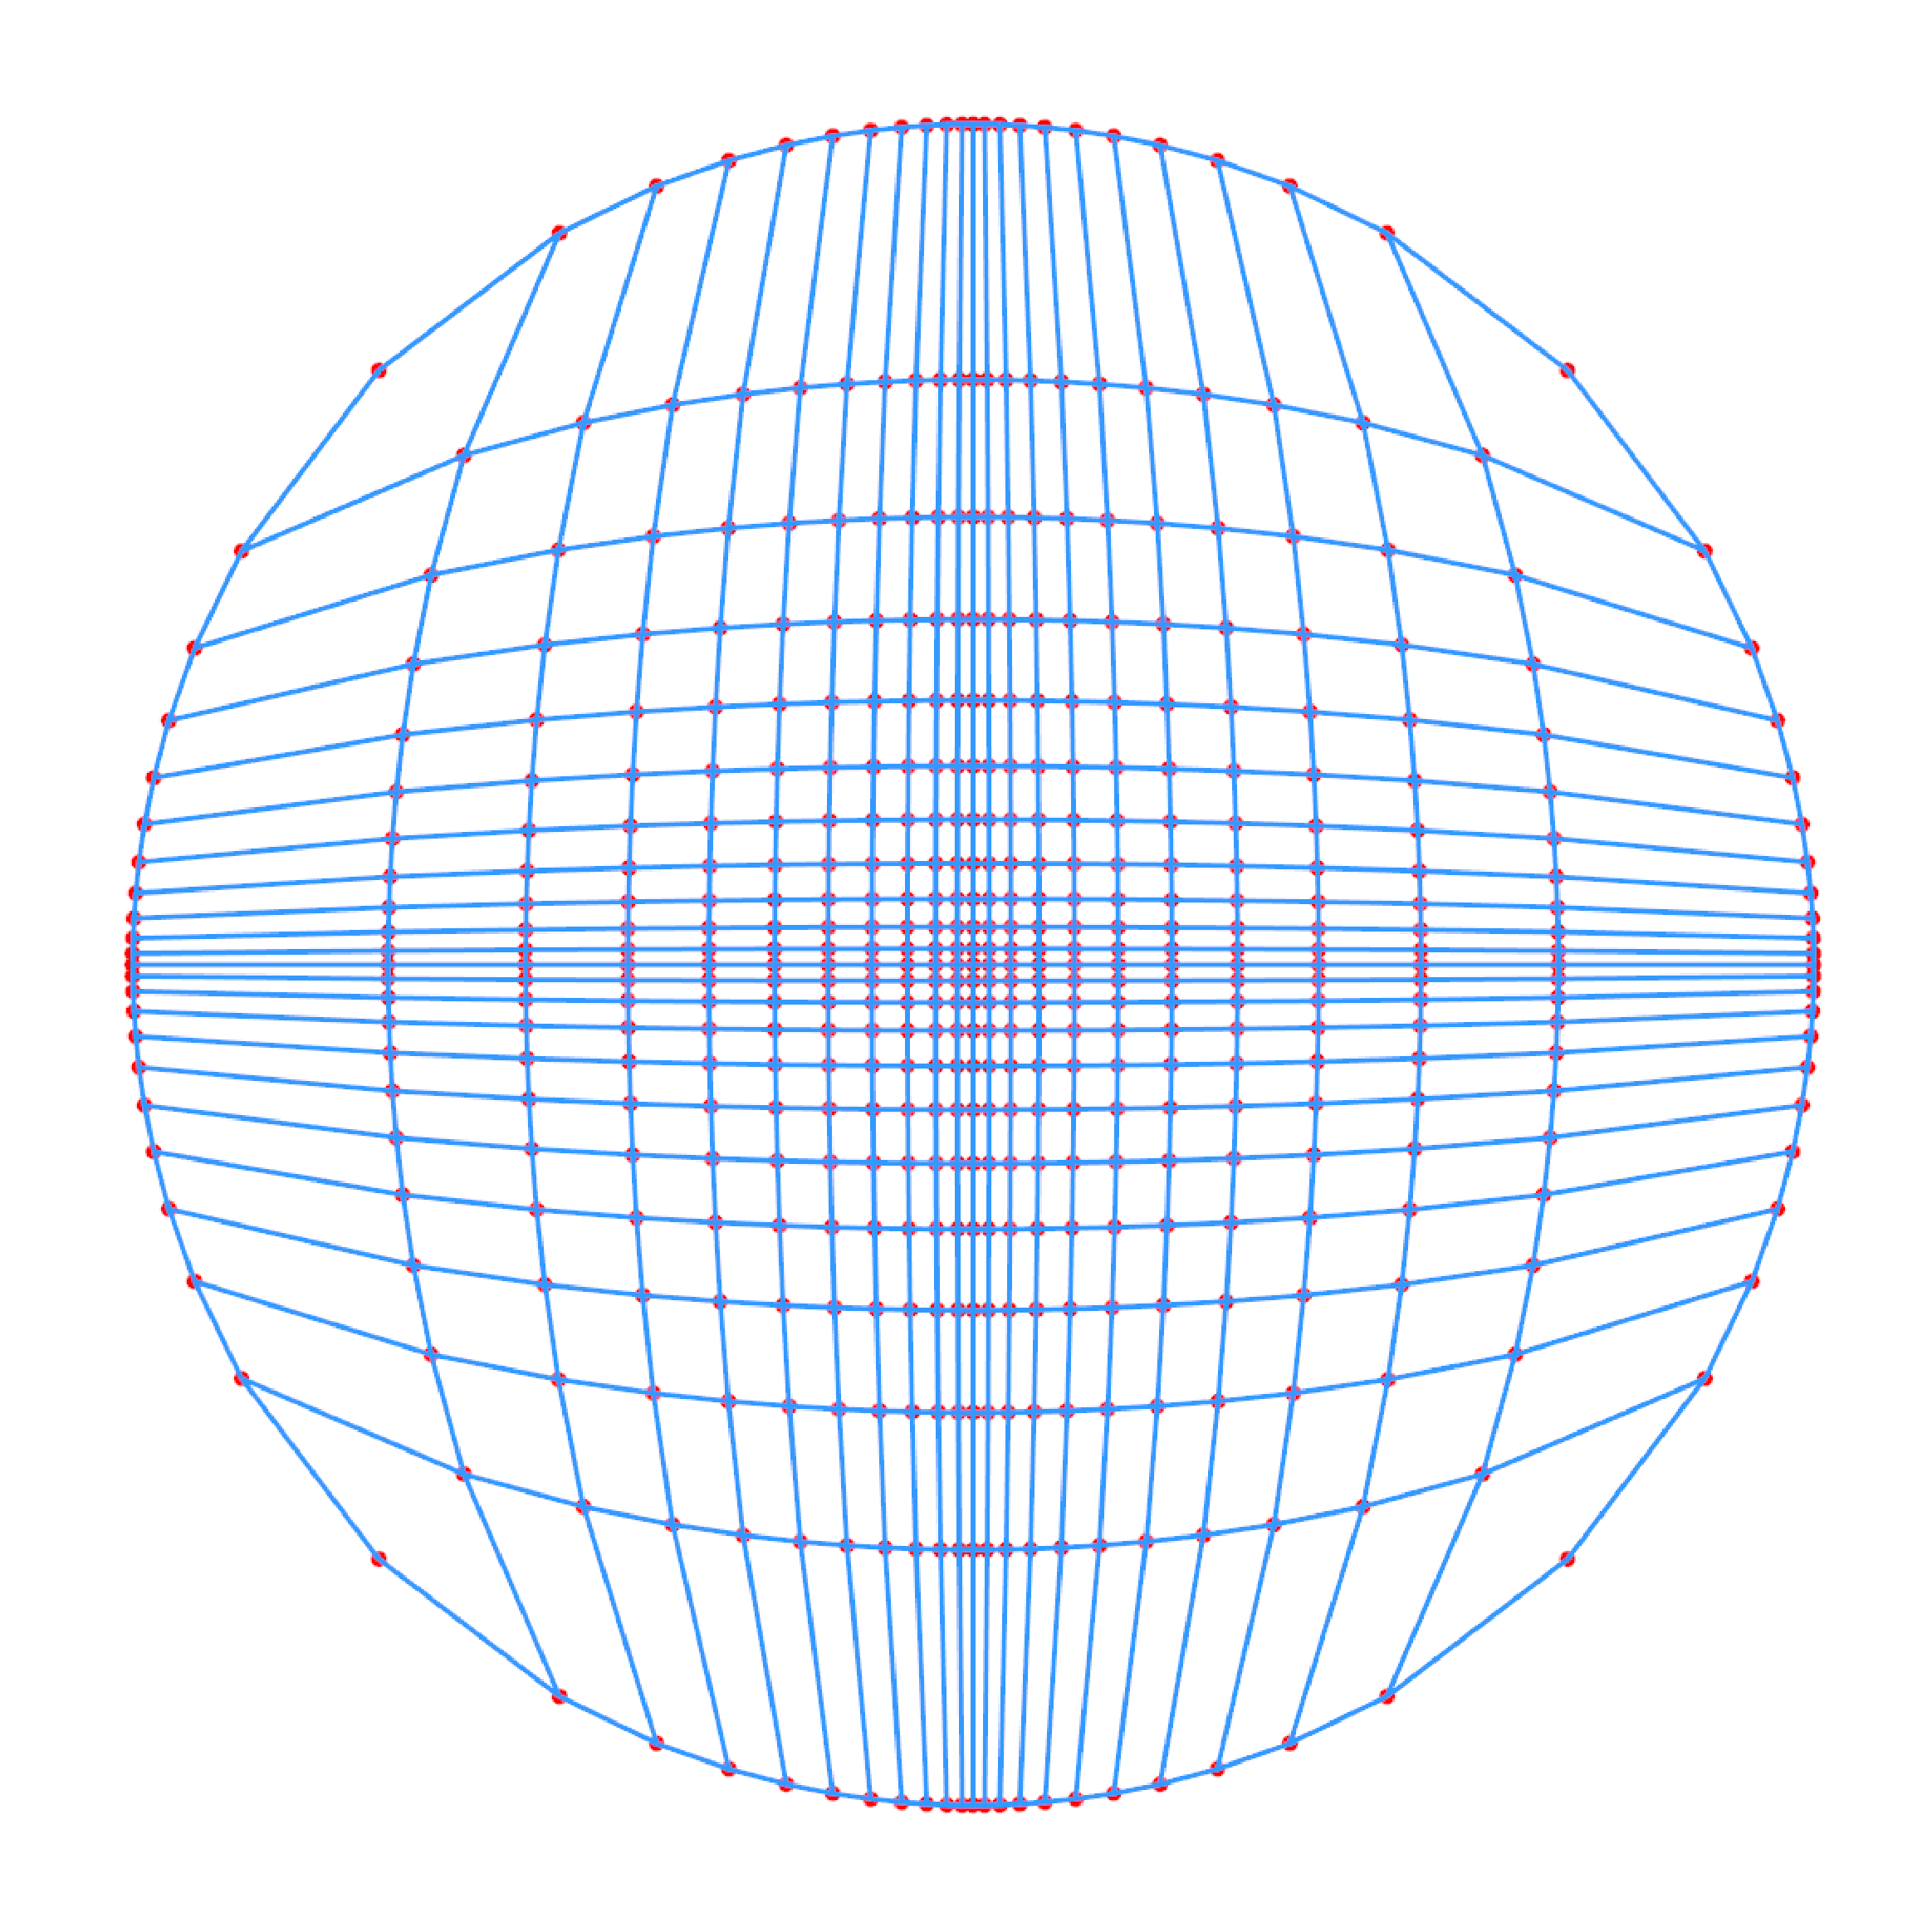
\epsfig{file = circle_s-rep.eps, width = 3cm}}
% \caption{A square grid transformed into a circle on the plane.}
% \label{fig:GridTypes} 
% \vspace{-0.1cm}
%\end{figure}

The following section explains how to project the transformed grid to the sphere.
Figure \ref{fig:SphereSamplingSphere} shows the results of mapping a regular-grid and log-grid on the sphere. 

\subsection{S-rep projection from the plane to the sphere}
\label{sec:StereographicProjection}

Once the ``circular log grid'' is created, the projection 
finds the corresponding positions on the sphere. 
Equation \ref{equ:stereoprojection} shows how the projection is done where $X = L(S(x'))$ and $Y = L(S(y'))$.

\begin{equation}  
	\begin{array}{lcc}
	    xs & = & 2X/(1 + X^2 + Y^2) \\
	    ys & = & 2Y/(1 + X^2 + Y^2) \\
	    zs & = & (-1 + X^2 + Y^2)/(1 + X^2 + Y^2)
	\end{array}
  \label{equ:stereoprojection}
\end{equation}

\begin{figure}[h!]
 \centering 
 \subfigure[Regular grid]{\epsfig{file = regularGridNorthPole.eps, width = 3.5cm}
			   \epsfig{file = regularGridSouthPole.eps, width = 3.5cm}}
 \subfigure[Log grid]{\epsfig{file = logGridNorthPole.eps, width = 3.5cm} 
		       \epsfig{file = logGridSouthPole.eps, width = 3.5cm}}
 \subfigure[Circular log grid]{\epsfig{file = circularLogGridNorthPole.eps, width = 3.5cm} 
		       \epsfig{file = circularLogGridSouthPole.eps, width = 3.5cm}}
		      
 \caption[Sphere's north and south pole sampling.]{The north (left) and south (right) poles are sampled using a regular,  a log grid and a circular log grid. 
						     The log grid sampling maps more points towards the south pole, and the circular grid 
						     produces the spherical cap opening in the representation.}
 \label{fig:SphereSamplingSphere}  
\end{figure}

Figure \ref{fig:SphereSamplingSphere} shows how the points from the regular grid and the log grid map 
on a sphere. The latter has better hub distribution on the sphere and produces a better s-rep of the cortex. 

Once the hub positions are sampled on the sphere, a fitting procedure to the spherical data provided by \textit{Freesurfer} is done.

\subsection{Fitting the s-rep to \textit{Freesurfer's} data}

At this point there are two spherical representations. 
The first one corresponds to a cortex;
the second one corresponds to the s-rep's SS.

To fit the s-rep to the spherical representation of the cortex,
each hub position is used as input to search for a set of closest points on 
the spherical representation of the cortex.
The searching procedure uses as standard closest neighborhood search algorithm 
with kd-trees. The kd-tree quickly locates the closest points on the sphere from \textit{Freesurfer}.

The folding procedure in the following section uses the points found
and their relationship to the GM and WM surfaces in order to fold the s-rep into the cortex.

\subsection{Folding the s-rep: from the sphere to the cortex}

%\begin{figure} 
% \centering 
% \subfigure[Circular grid]{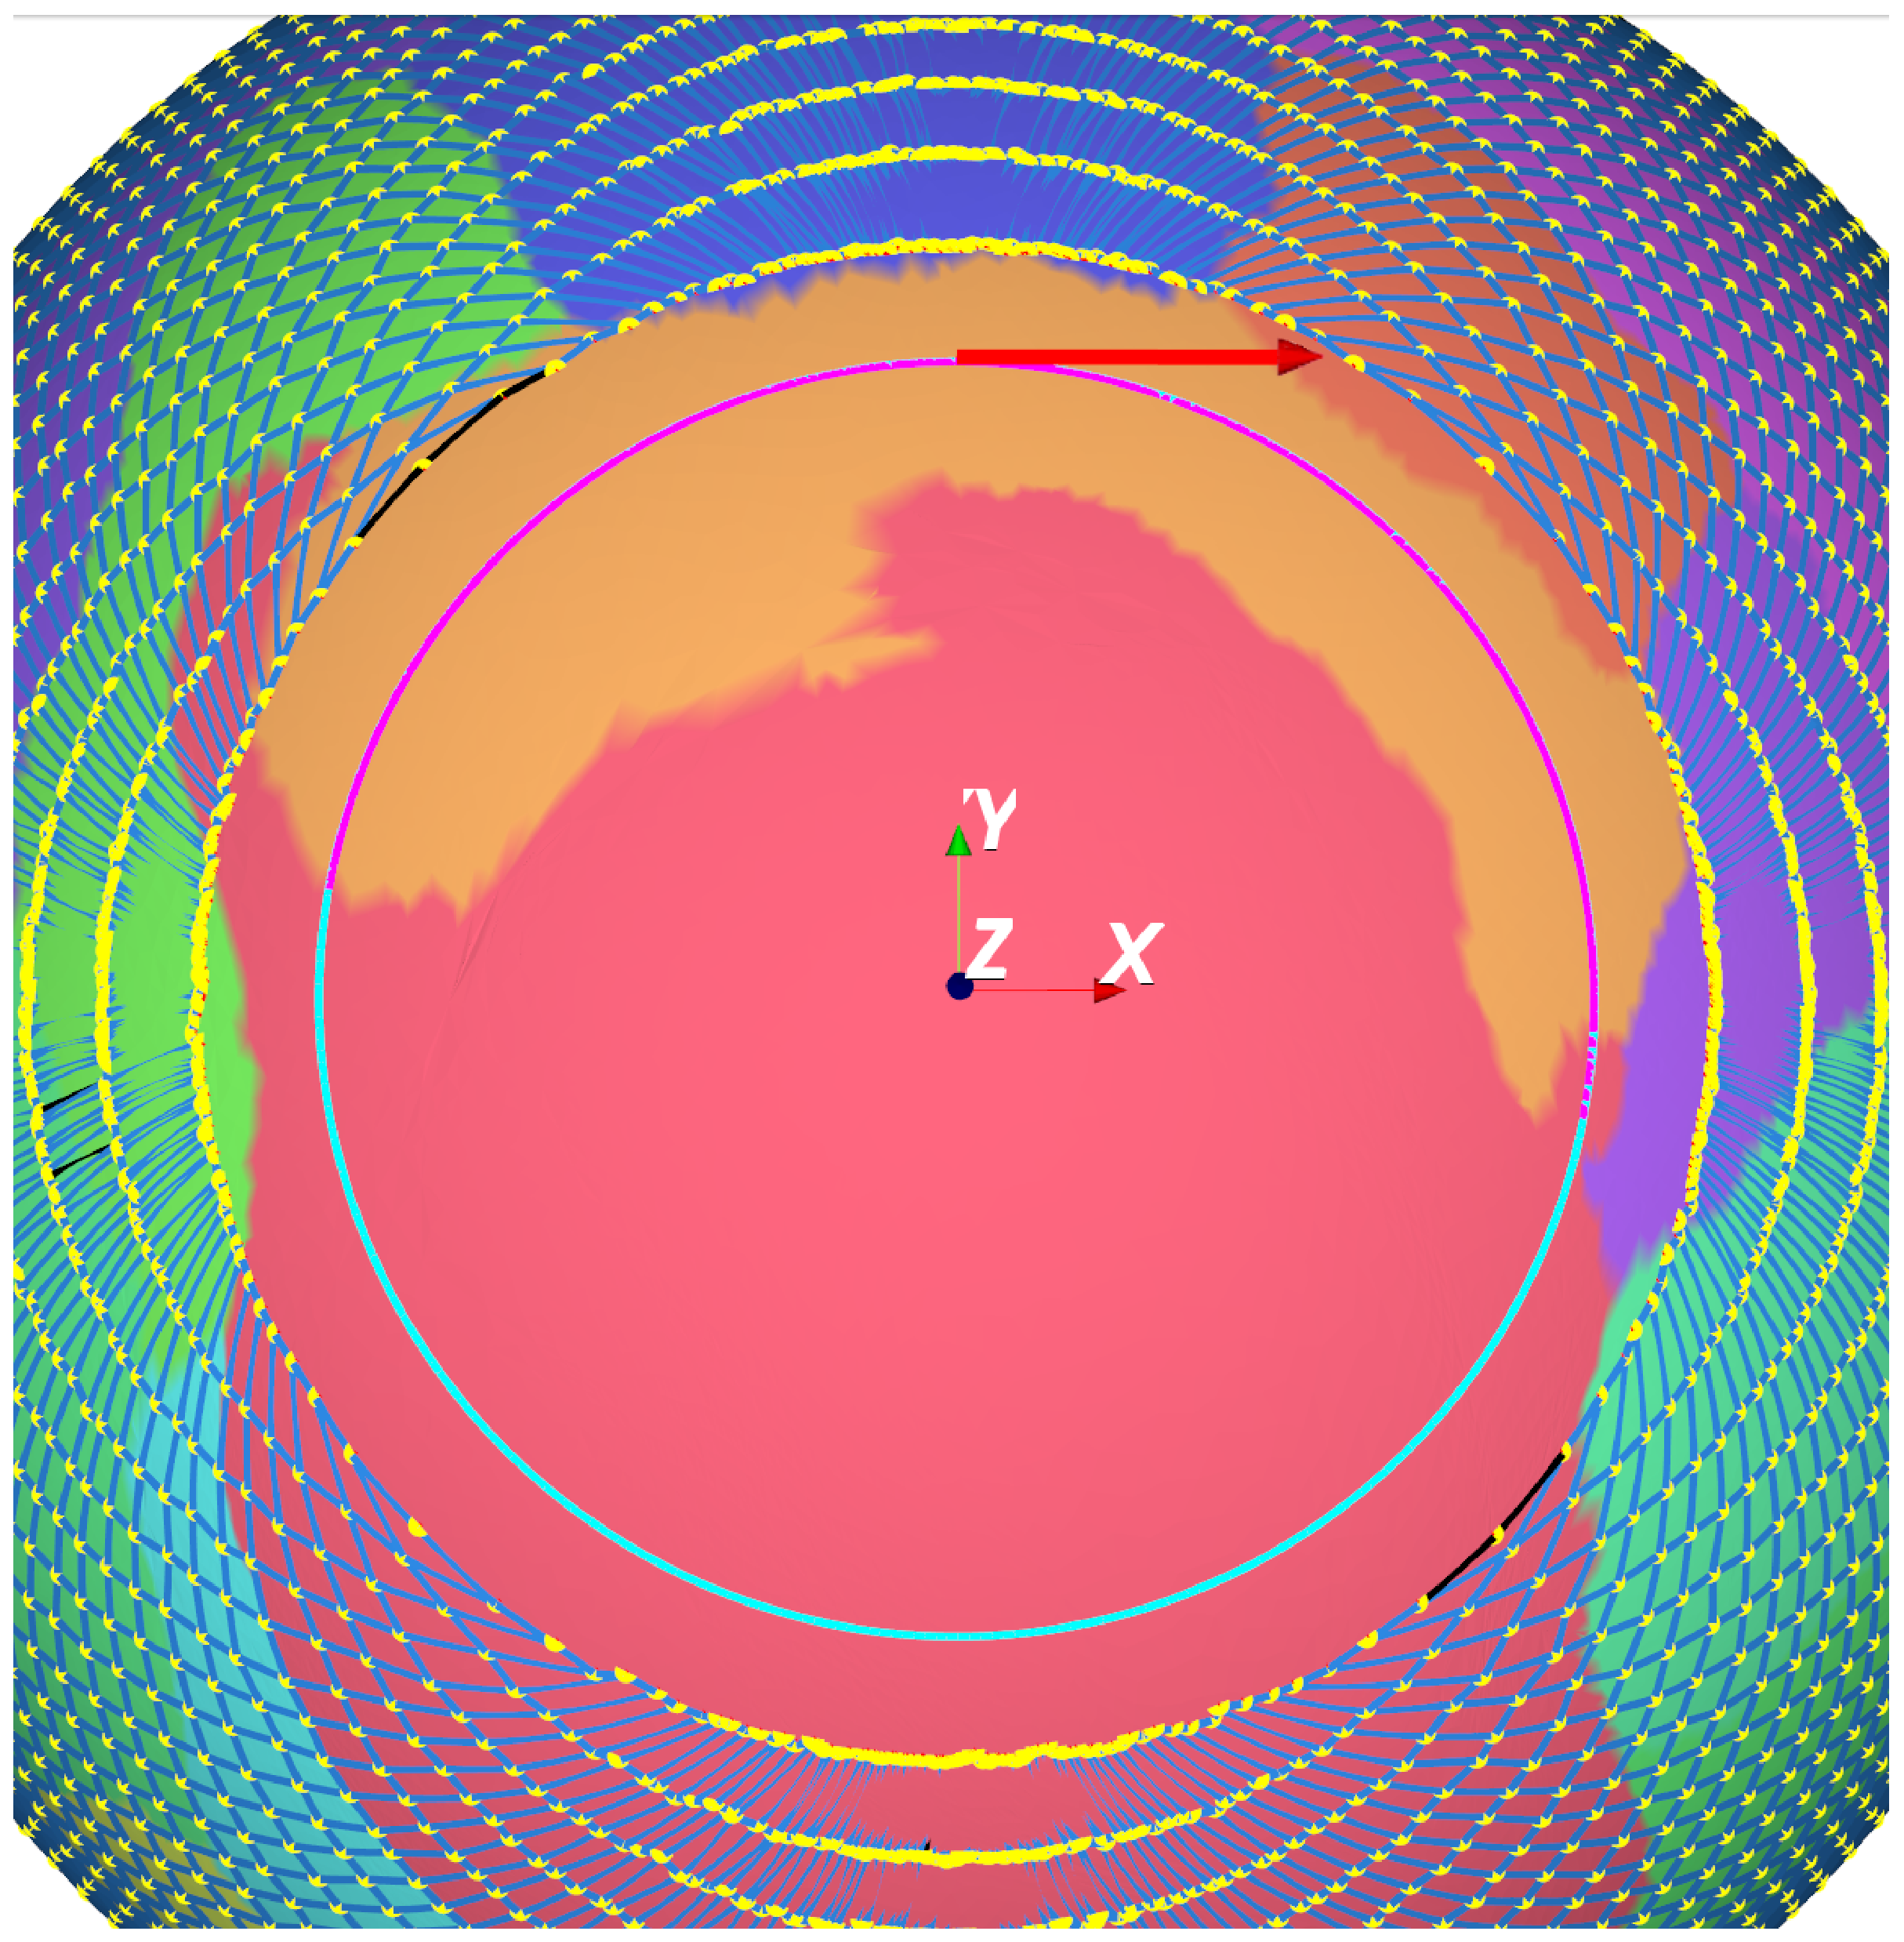
\epsfig{file = fittedSrepSphereCircularGrid.eps, width = 2.75cm}
%			   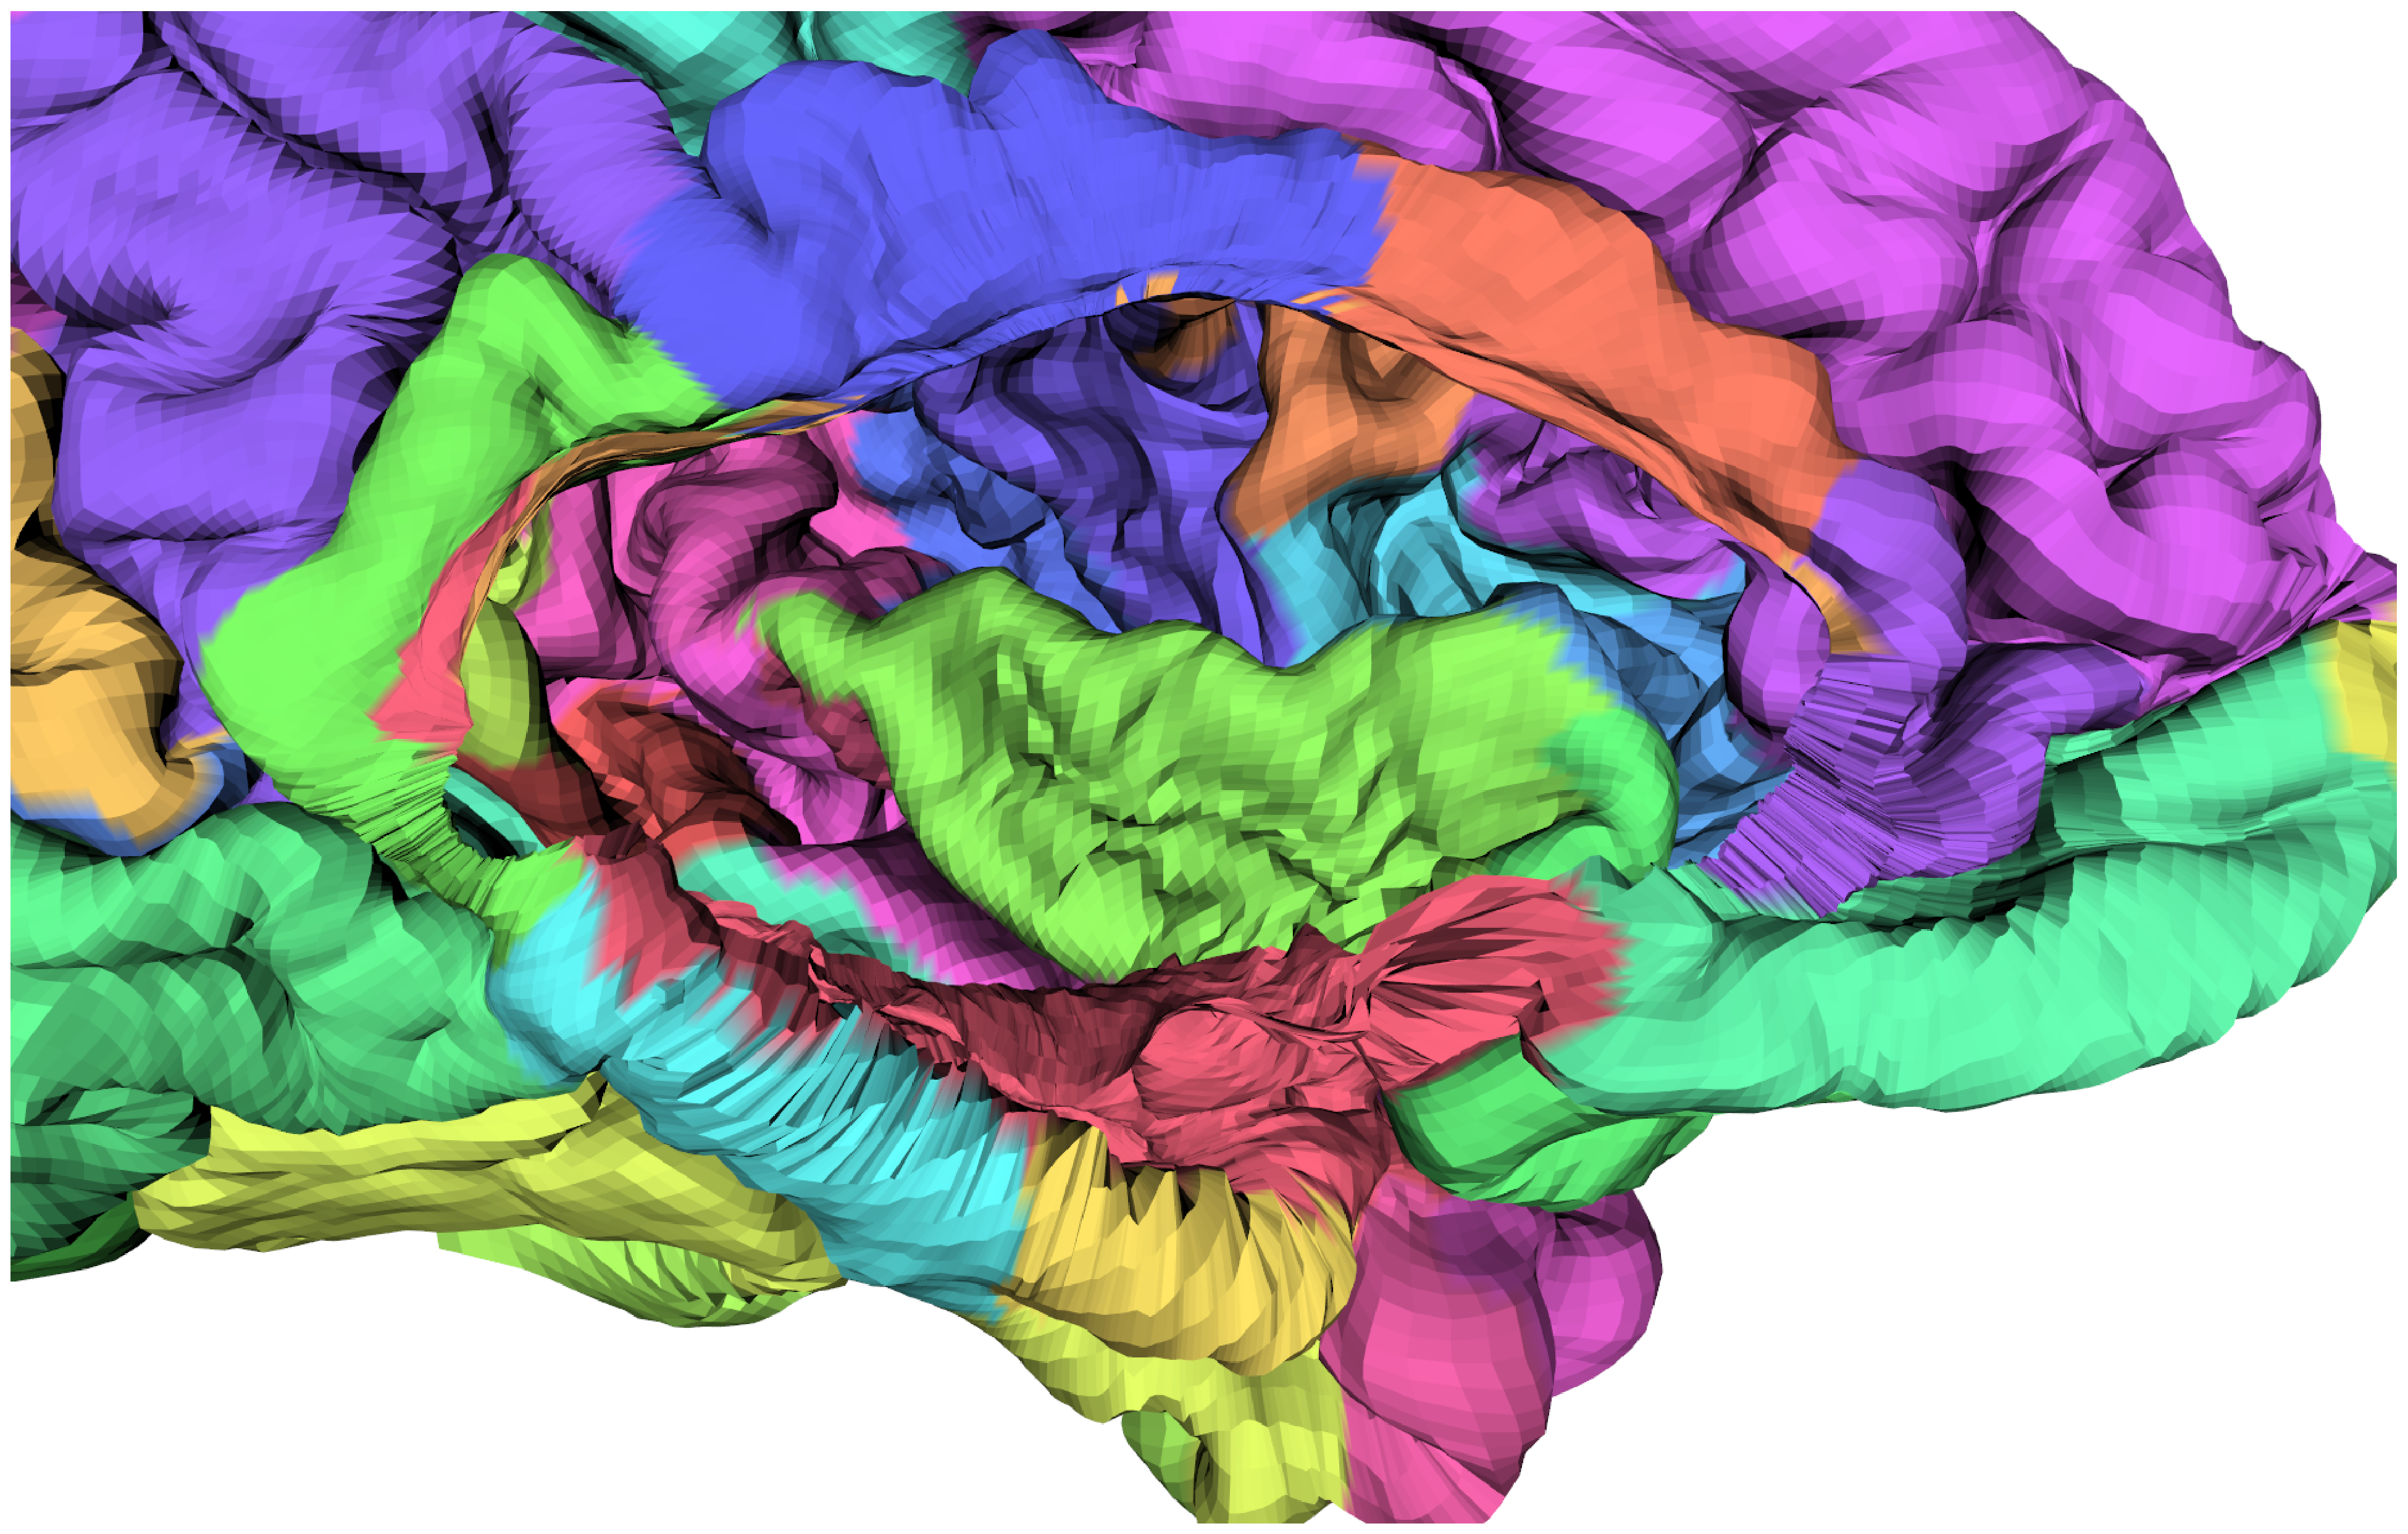
\epsfig{file = fittedSrepCircularGrid.eps, width = 3cm}}
% \subfigure[Square grid]{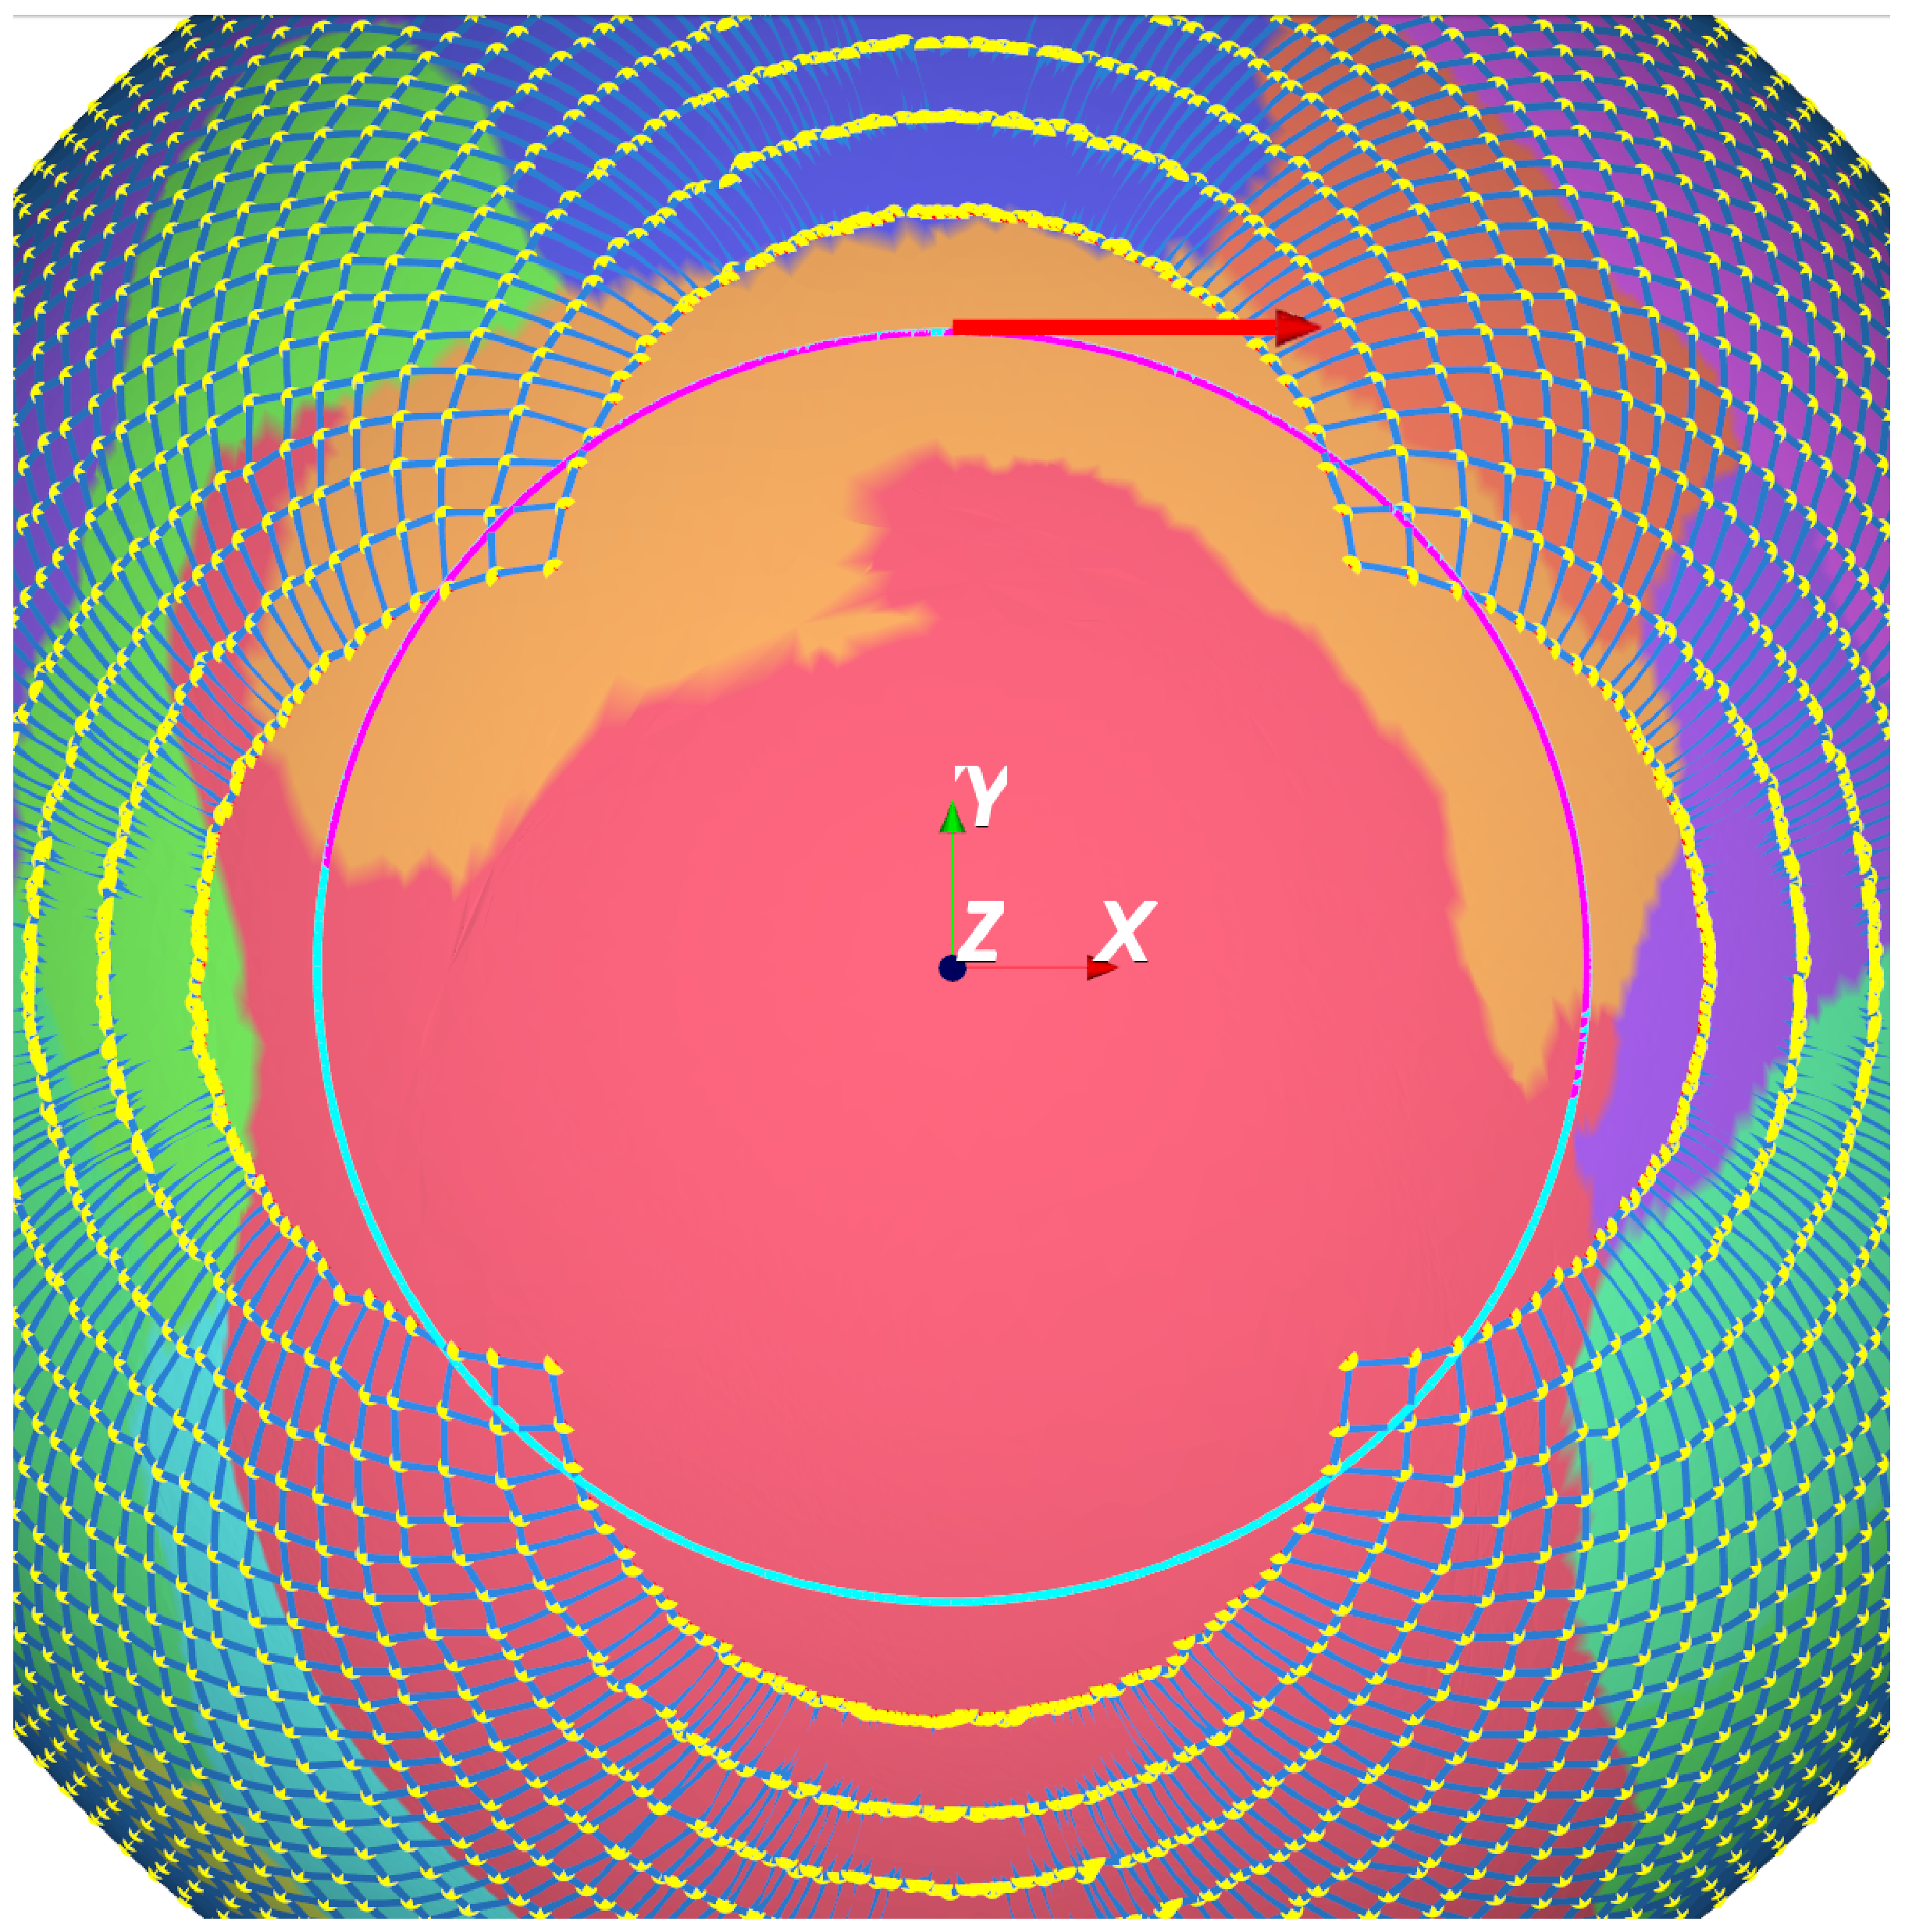
\epsfig{file = fittedSrepSphereSquareGrid.eps, width = 2.75cm} 
%		       \epsfig{file = fittedSrepSquareGrid.eps, width = 3cm}} 
% \caption{The best circle is shown in cyan, the projected points in magenta (on top of the best circle).
%	  The north pole is the center point of the best fitting circle, it is used to rotate the sphere to the north pole. 
%	  The mean of the projected points is found on the circle and is used to calculated a tangent, which is later used to 
%	  calculate a second rotation to align the data with the x axis. On figure (b), the regions highlighted in red correspond 
%	  to the corners of the grid.}
% \label{fig:BestCircle}  
%\end{figure}

The s-rep is folded into the cortex
using the points found on the sphere and
the cortical widths given by \textit{Freesurfer}. 

The following penalties minimize an objective function for each hub:

\begin{enumerate}
 \item The hub's distance to the GM and WM surfaces (~half the cortical width).
 \item The top spoke's tip distance to the GM surface.
 \item The bottom spoke's tip distance to WM surface.
 \item The normal of the SS (see Equation \ref{equ:sheetNormal}) to the normal of the WM surface.
 \item The normal of the SS to the normal of the GM surface.
\end{enumerate}


%\begin{equation}
% \hat{s_{rep}(i)} = \operatorname*{Arg\,min}_{p_i, s^{-1}_i, s^1_i} \sum_{j=1}^{k} || Cp(j) - p_i || + \left \{ \begin{array}{ll}
%                                                                                                                 ||Cp(j) - (p_i +  s^{-1}_i)||, & Cp(j) \in WM \\
%                                                                                                                 ||Cp(j) - (p_i +  s^{1}_i)||, & Cp(j) \in GM
%                                                                                                                \end{array} \right .
%                                                                                                     + || (s^{1}_i - s^{-1}_i) - NCp(i) ||
%\end{equation}

The procedure folds back the s-rep that was sampled on the spherical space to the original shape of the cortex. 
After the folding, the topology of the s-rep is preserved. 
In other words, each of the quads that build the skeletal structure 
are correctly oriented on the folded form of the cortex. 
Moreover, both top and bottom spokes point towards the GM and WM surfaces respectively. The width of the
spokes is also determined.

The interpolation mechanisms described in Section \ref{sec:s-repImplementation} can 
be used to produce the WM and GM surfaces. 
Since the implied surfaces are not equivalent to the original ones, the following section evaluates 
their quality. 

\section{Evaluation of the implied GM and WM surfaces}
\label{sec:Evaluation}

To evaluate if the surfaces are close enough to the original ones, 
a tool known as \textit{Meshvalmet} is used.
The tool uses the Hausdorff distance to estimate the difference between discrete 3D surfaces. 
The approach is based on \cite{aspert_mesh:_2002}. It
calculates the mean distance error from each vertex of the reference surface to 
a target one, in this case, the interpolated surface against the original surface. 
The comparison is done separately on the GM and WM surfaces.
The sampling step is set to $0.1$ and an absolute distance measure is used.
By lowering the sampling step and using the 
absolute distance, the accuracy of \textit{Meshvalmet} is increased.

Analyzing the results of \textit{Meshvalmet} 
yields a set of parameters to generate the best possible representation 
for all subjects. 
The parameters to set for the s-rep are size and sampling step on the sphere.
The following section analyzes the size of the s-rep.

\subsection{Best s-rep size}
\label{sec:s-repsize}

\begin{figure}[!h]
 \centering 
 \subfigure[GM surface]{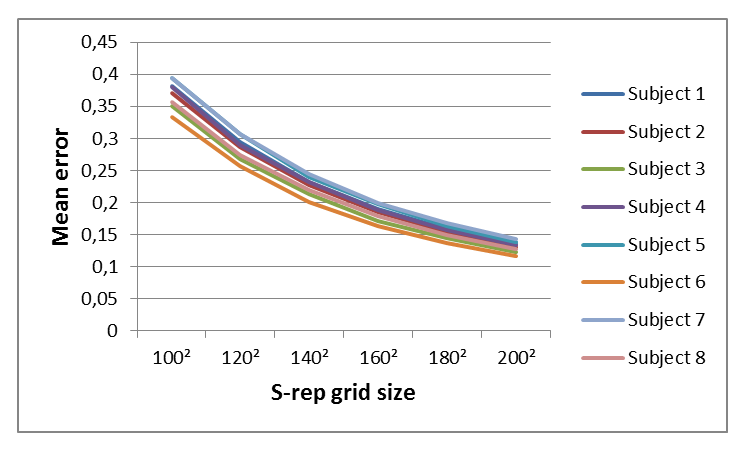
\epsfig{file = lh_greyMatterGridSize.eps, width = 7.25cm}}
 \subfigure[WM surface]{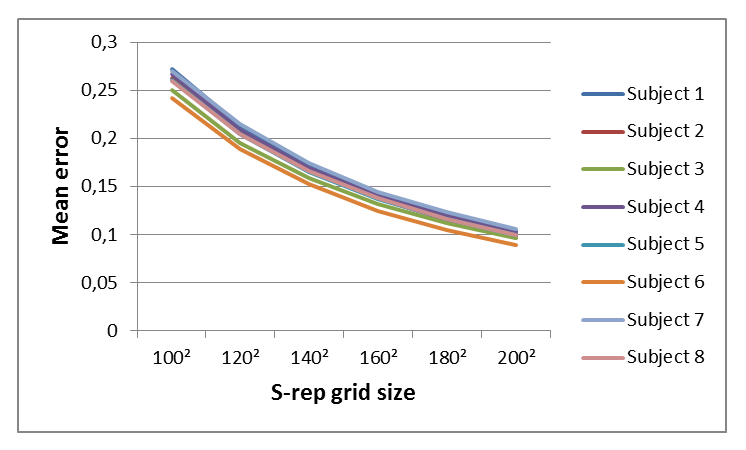
\epsfig{file = lh_whiteMatterGridSize.eps, width = 7.25cm}}
 \caption[GM and WM surface mean error: grid size.]{Mean error using different grid size of the s-rep.}
 \label{fig:GridSize} 
\end{figure}

The first parameter to set is the size of the s-rep. This is based on different criteria
such as reducing the number of points in the original data. A typical cortical surface contains $130,000+$ vertex.
By using an s-rep of $160^2$ atoms, the information is reduced by $~40\%$, \textit{i.e}, 
$76.800$ tuples including the hub positions plus both spoke directions.
%Reducing the information not only allows to produce compact representation of the data but it also allows the use of new statistical tools.

Figure \ref{fig:GridSize} shows the mean error using s-reps of different sizes, tested on 8 different subjects. 
The following analysis uses a grid of $160^2$ atoms for all cases.

\subsection{Best s-rep sampling}
\label{sec:minvalue}

The second parameter to set is the initial value for the log scale sampling on the grid.
This parameter controls how the hubs will distribute on the sphere. A value close to $0$ will 
map a larger number of points towards the south pole. 
Figure \ref{fig:AverageCell} shows the average area of the quads that compose the skeletal locus of the s-rep and their SD (standard deviation).
Notice that for values greater that $0.04$, the SD increases rapidly.
Figure \ref{fig:InitialLogValue} shows the mean error of the interpolated surfaces for different $Min$ values.
According to the analysis, values between $0.01$ and $0.4$ seem reasonable as 
the minimum error overall cases for the surfaces is found inside this range.
The $Min$ value is set to $0.02$
in order to increase the regularity of the quads and 
lower the mean error of the surface.
This value produces the best results over all subjects used in the analysis. 

\begin{figure} 
 \centering  
 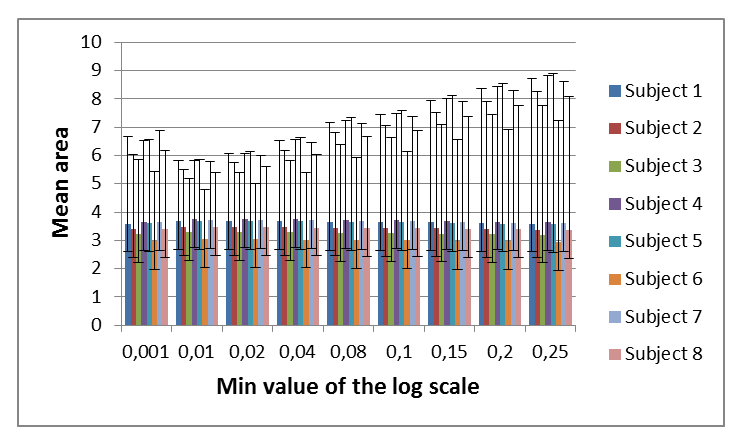
\epsfig{file = lh_averageCellArea.eps, width = 9cm}
 \caption[Average area of an srep's quad.]{Average quad area of the s-rep with standard deviation for different $MIN$ values of the log scale.}
 \label{fig:AverageCell}  
\end{figure}

\begin{figure} 
 \centering 
 \subfigure[GM surface]{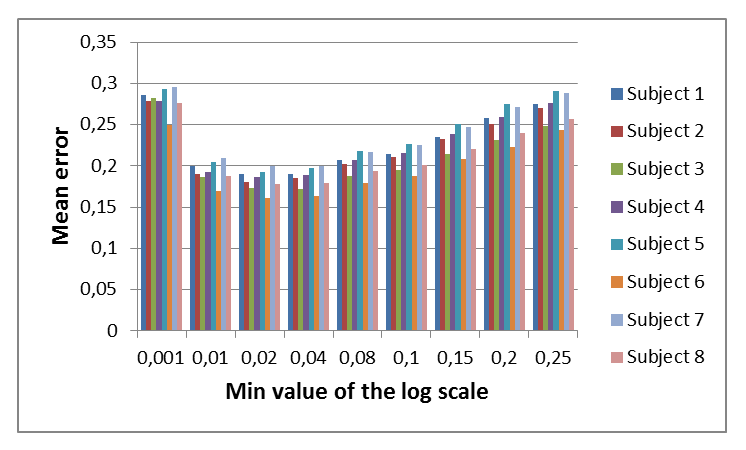
\epsfig{file = lh_greyMatterLogScale.eps, width = 7.25cm}}
 \subfigure[WM surface]{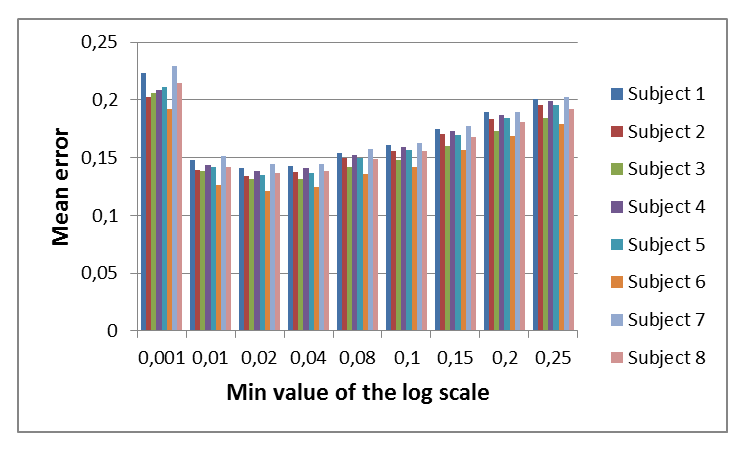
\epsfig{file = lh_whiteMatterLogScale.eps, width = 7.25cm}}
 \caption[GM and WM surface mean error: log scale.]{Mean error of the GM and WM surfaces for different $MIN$ values of the log scale.}
 \label{fig:InitialLogValue} 
\end{figure}


Figure \ref{fig:InterpolatedCortex} shows the interpolated cortex for both hemispheres. 
The coloring on the surfaces are set according to the cortical
parcellation of the neuroanatomical structures at each location in the cortex. 
%Each atom has the corresponding label found on the spherical surface.
%During the interpolation, each new point is labeled according to a voting scheme using the labels of the closest neighboring atoms.

\begin{figure}
 \subfigure[Original surfaces.]{\epsfig{file = lh_whiteMatterOriginal.eps, width = 8cm}
			   \epsfig{file = rh_whiteMatterOriginal.eps, width = 8cm}}
 \subfigure[Interpolated surfaces.]{\epsfig{file = lh_whiteMatterInterpolated.eps, width = 8cm}
			   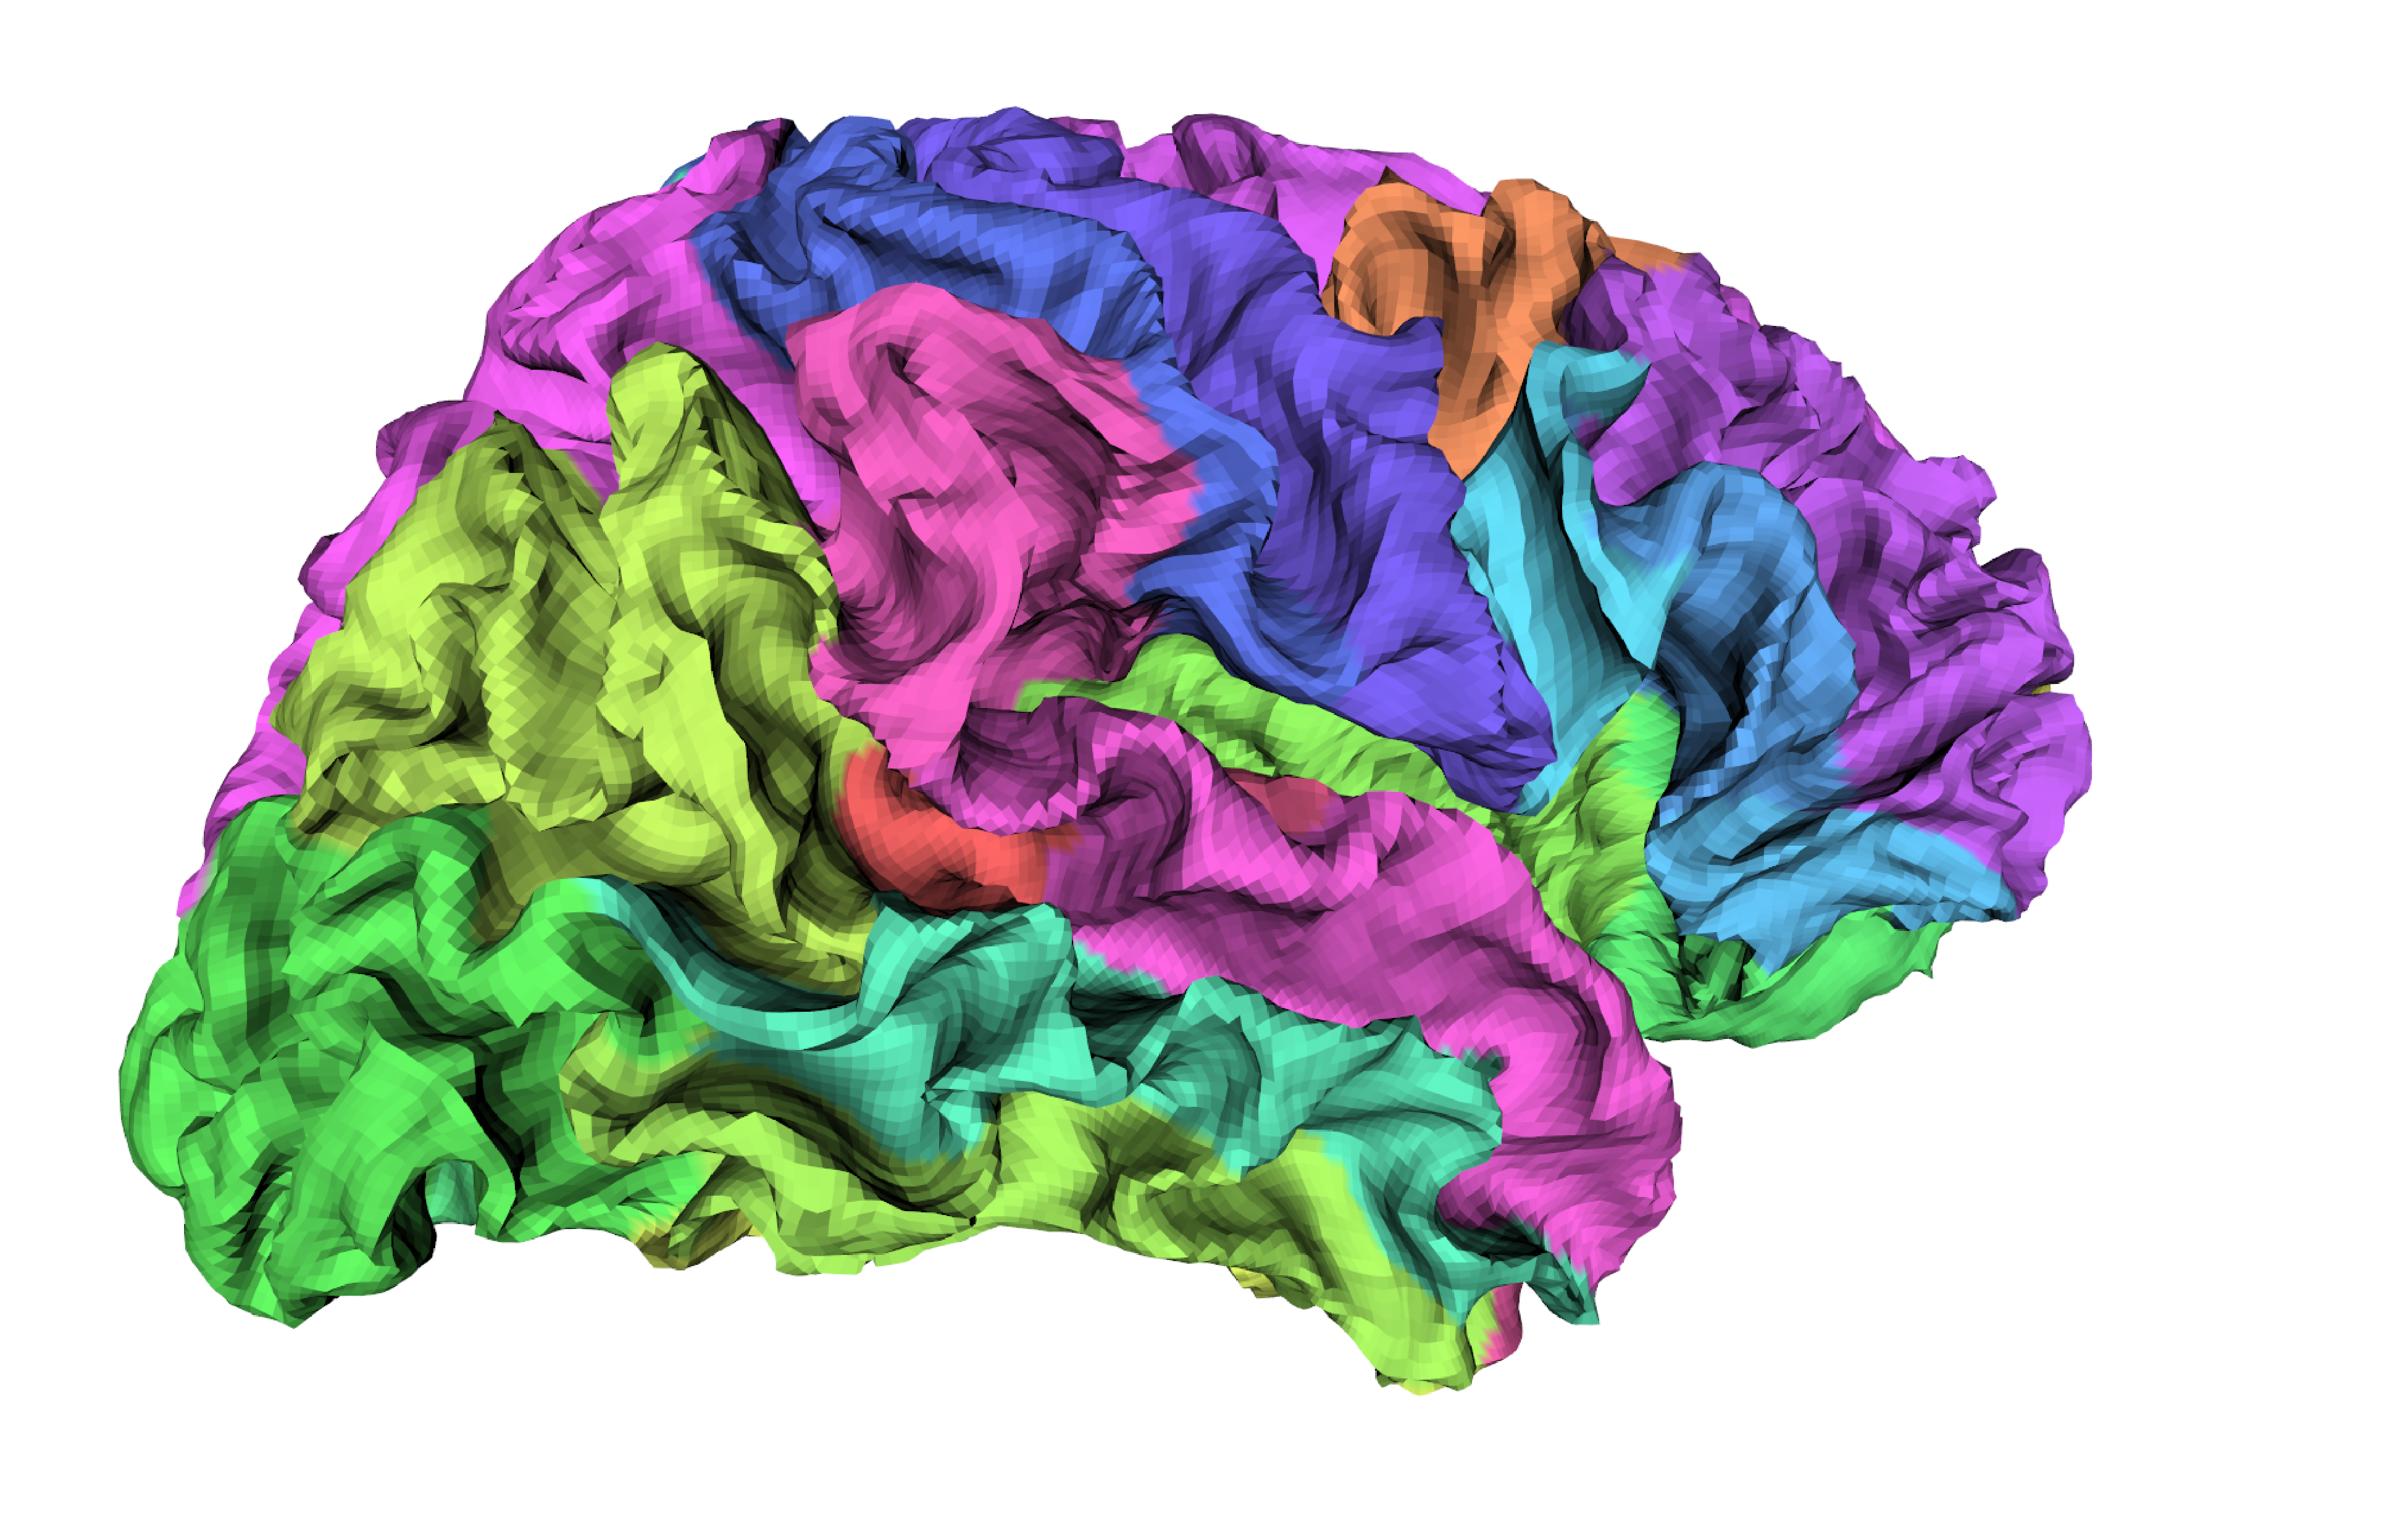
\epsfig{file = rh_whiteMatterInterpolated.eps, width = 8cm}}
 \caption[Comparison of the interpolated and original WM surfaces.]{Comparison of the original and interpolated WM surfaces for the left and right hemispheres.
	  The s-rep has $160^2$ atoms. The interpolated surfaces seem to have wrinkles at some places 
				      but according to the error measurement, they are close to the original ones. 
	                             Moreover, modeling the cortex via s-reps offers new capabilities such as the local coordinate system inside the structure.
	                             This new set of capabilities are not available in the regular representation.}
 \label{fig:OriginalCortex}
\end{figure}
\begin{figure} 
 \subfigure[Original surfaces.]{\epsfig{file = lh_greyMatterOriginal.eps, width = 8cm}
				  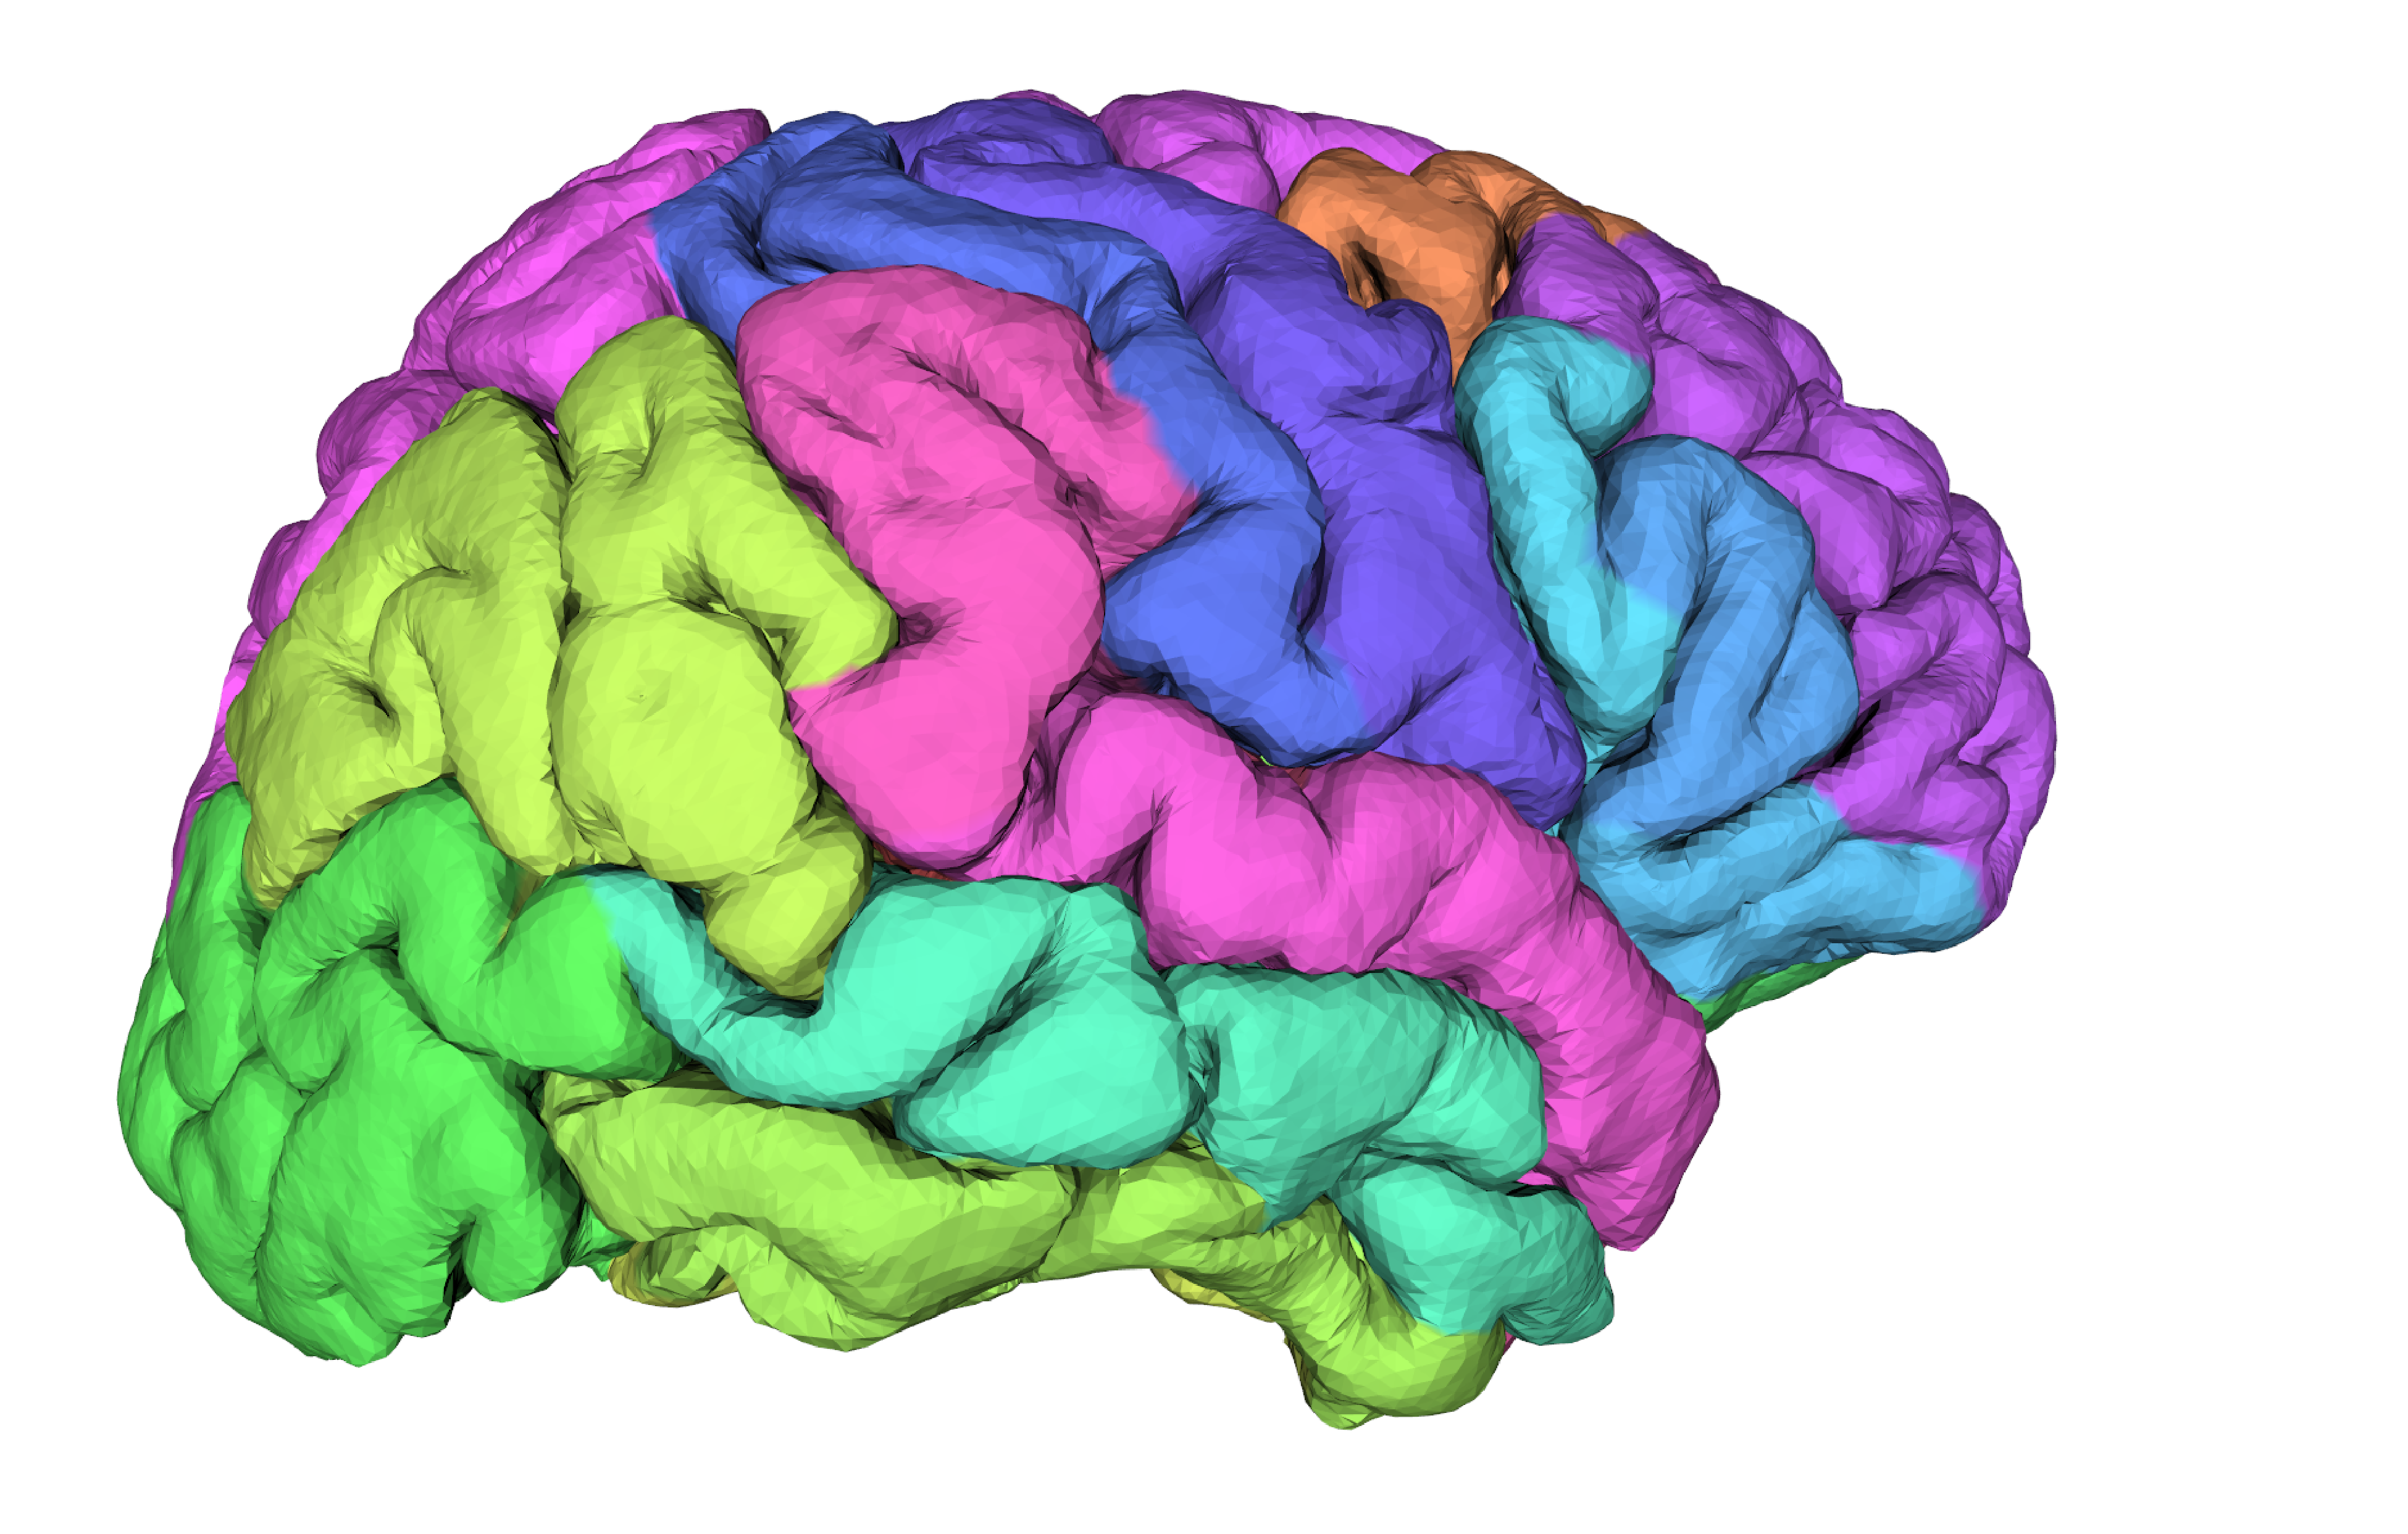
\epsfig{file = rh_greyMatterOriginal.eps, width = 8cm}}
 \subfigure[Interpolated surfaces.]{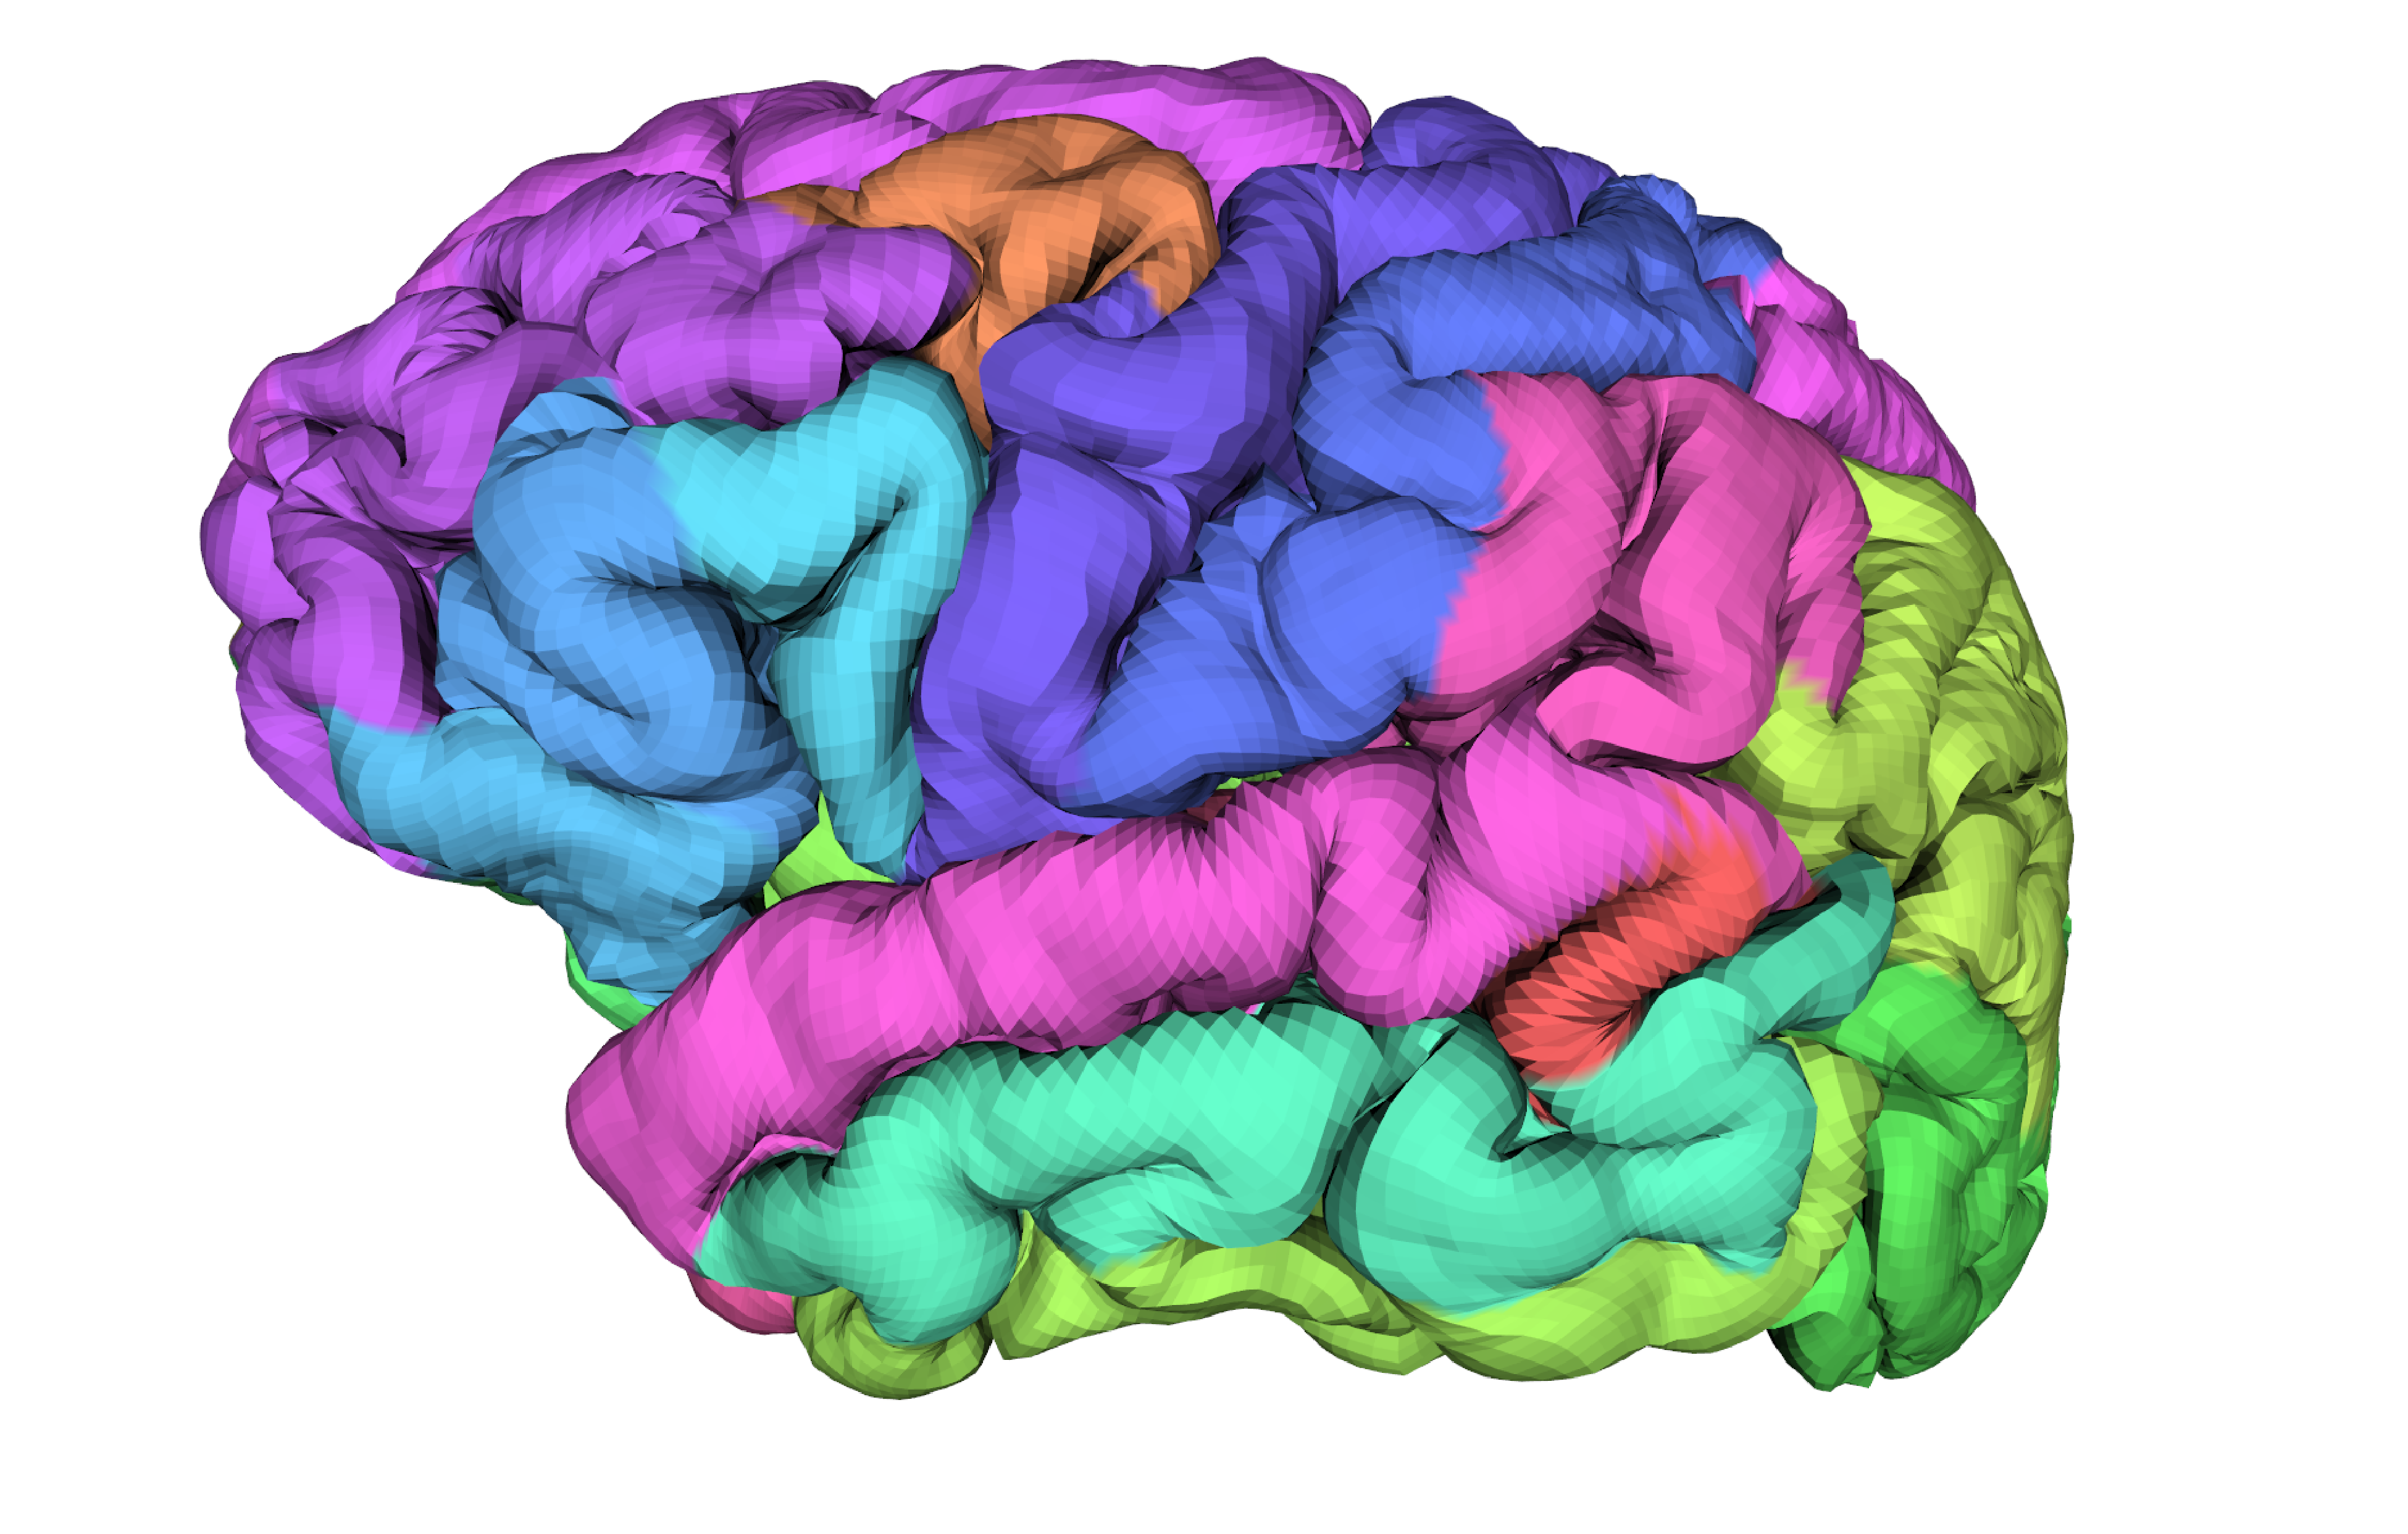
\epsfig{file = lh_greyMatterInterpolated.eps, width = 8cm}
				  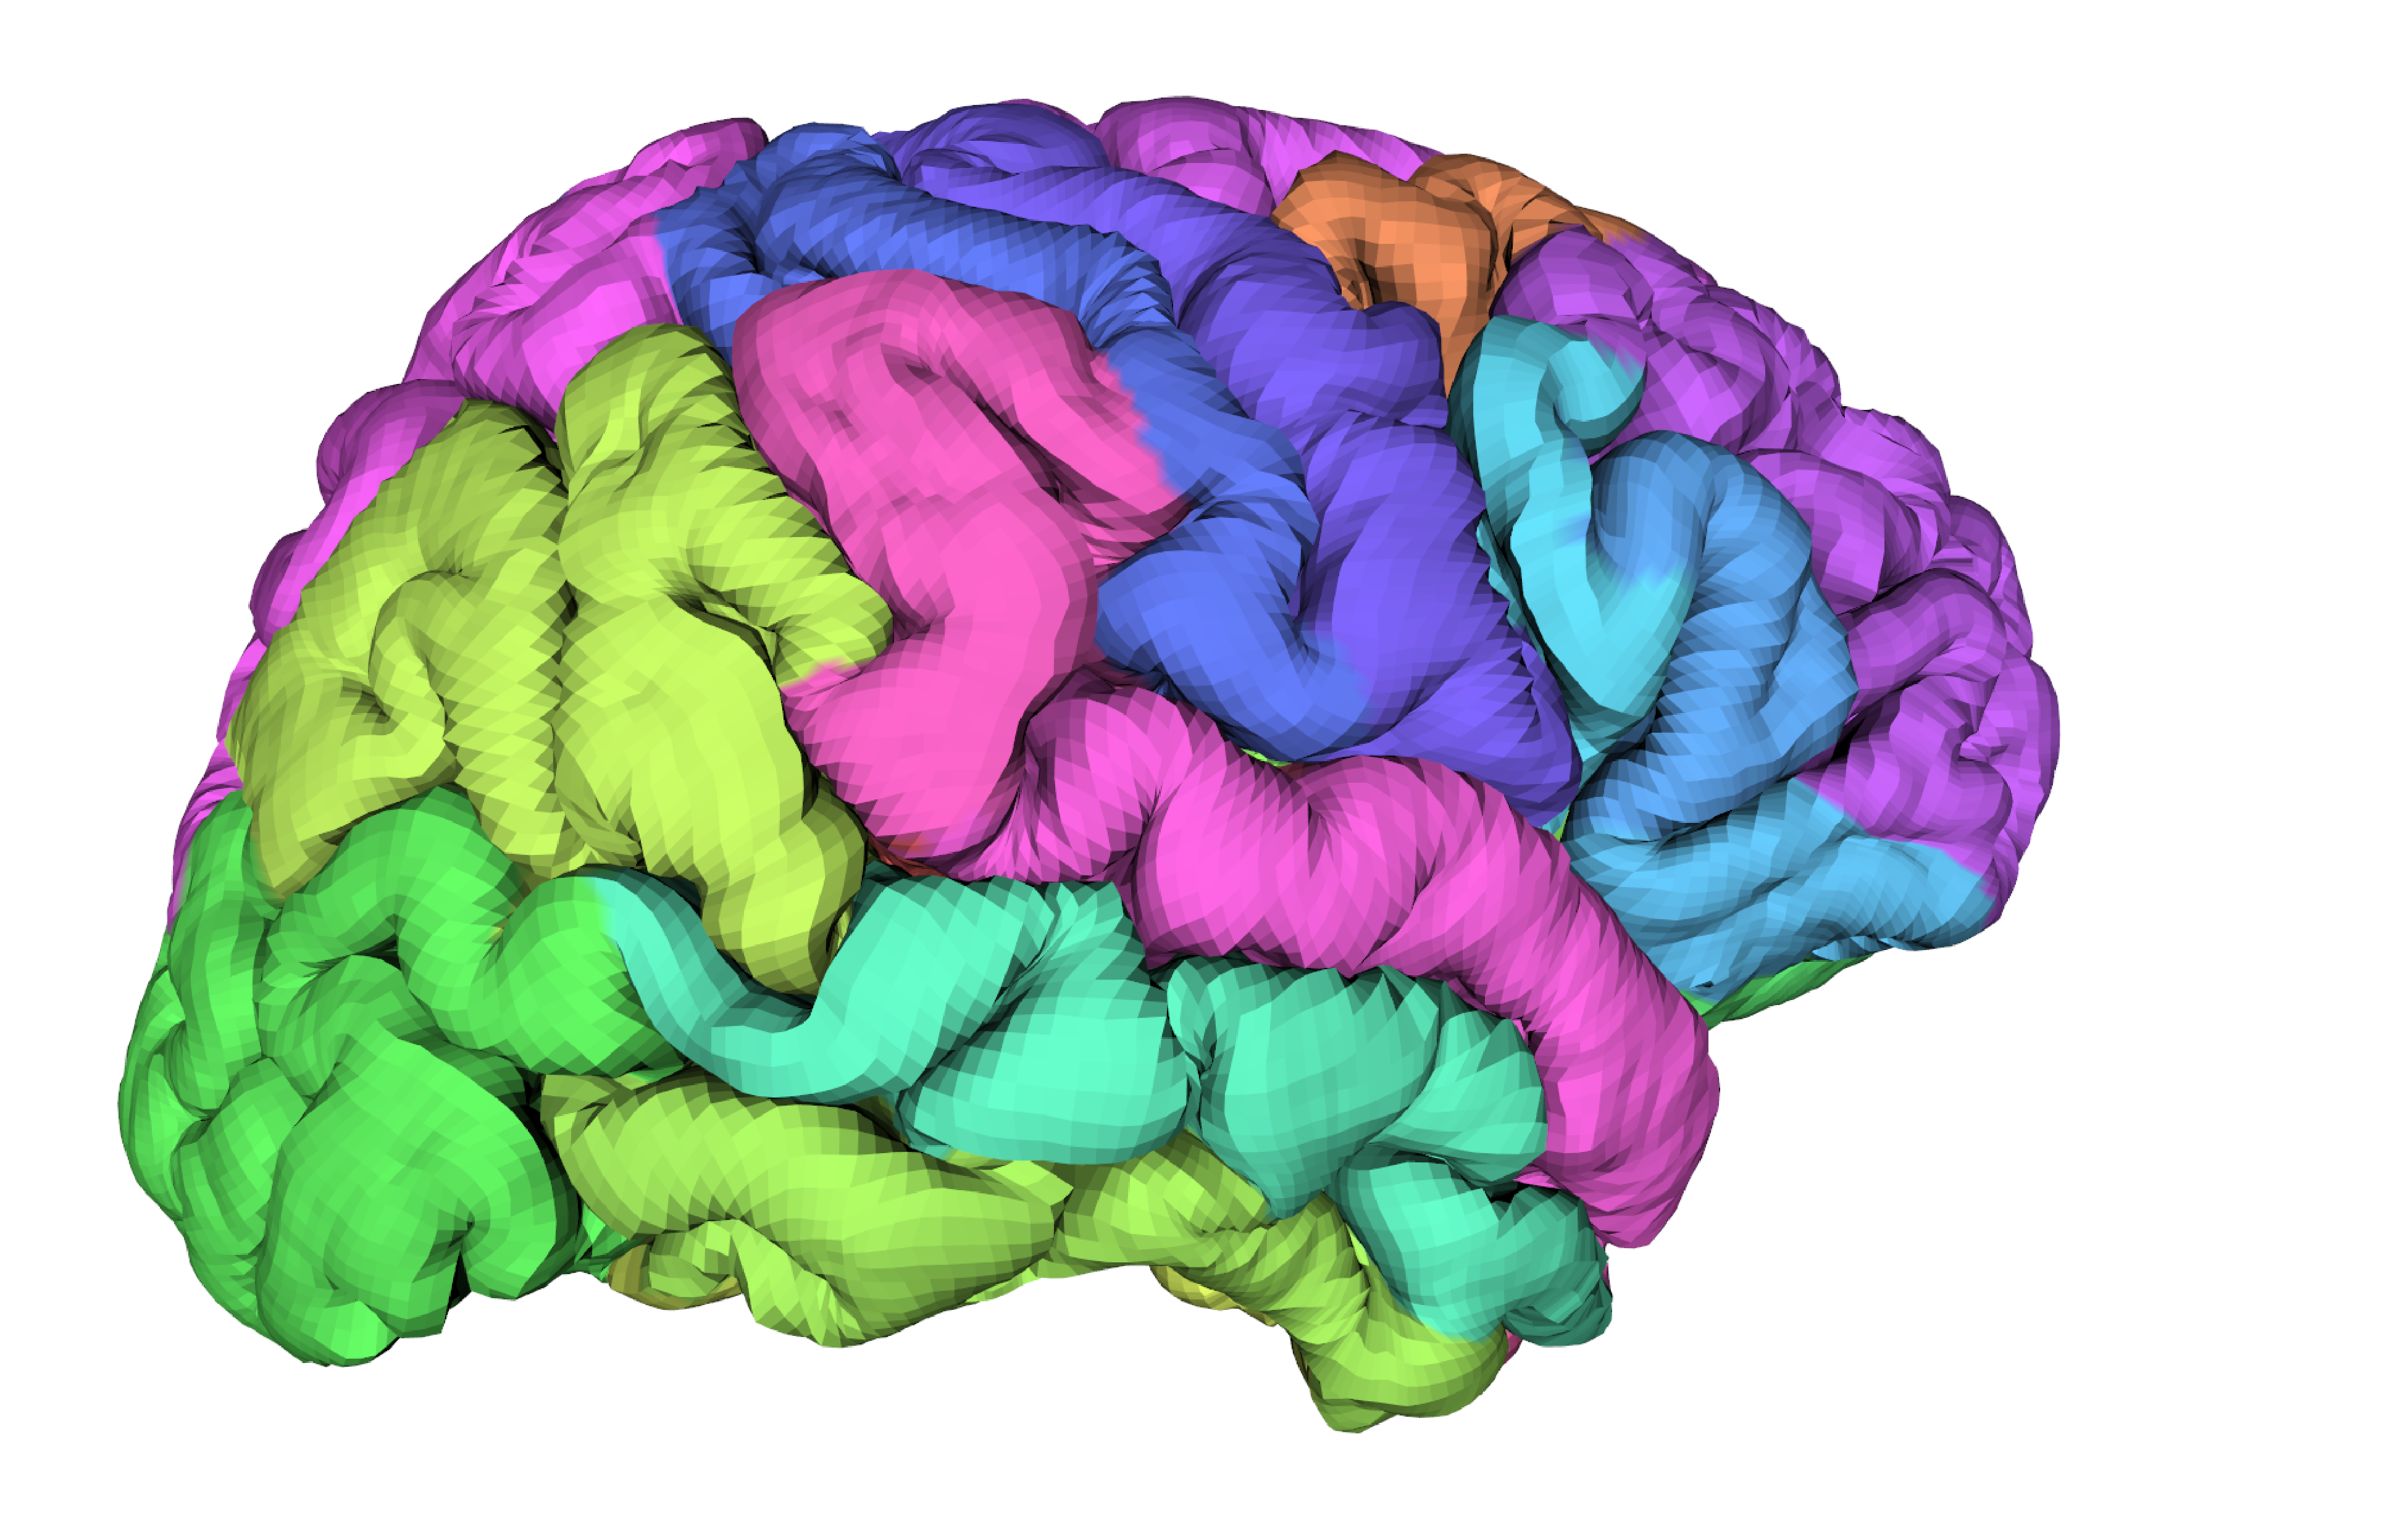
\epsfig{file = rh_greyMatterInterpolated.eps, width = 8cm}}
 \caption[Comparison of the interpolated and original GM surfaces.]{Comparison of the original and interpolated GM surfaces for the left and right hemispheres.			
	The s-rep has $160^2$ atoms. The interpolated surfaces seem to have wrinkles at some places 
				      but according to the error measurement, they are close to the original ones. 
	                             Moreover, modeling the cortex via s-reps offers new capabilities such as the local coordinate system inside the structure.
	                             This new set of capabilities are not available in the regular representation.}
 \label{fig:InterpolatedCortex}  
\end{figure}

In the following section, the s-rep of the cortex is used to evaluate
the changes of cortical width using synthesized data from a base model. 

%\begin{figure}
% \vspace{-0.2cm}
% \centering 
% \subfigure[Gray matter surface]{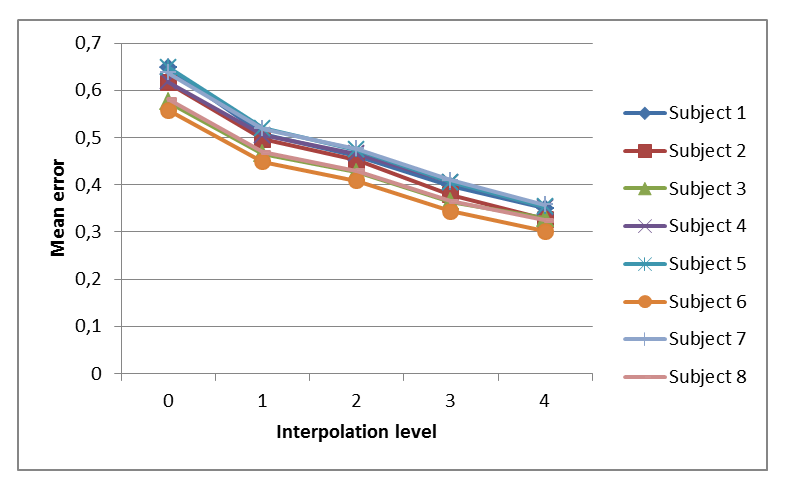
\epsfig{file = lh_greyMatterInterpolationLevel.eps, width = 6cm}}\\
% \subfigure[White matter surface]{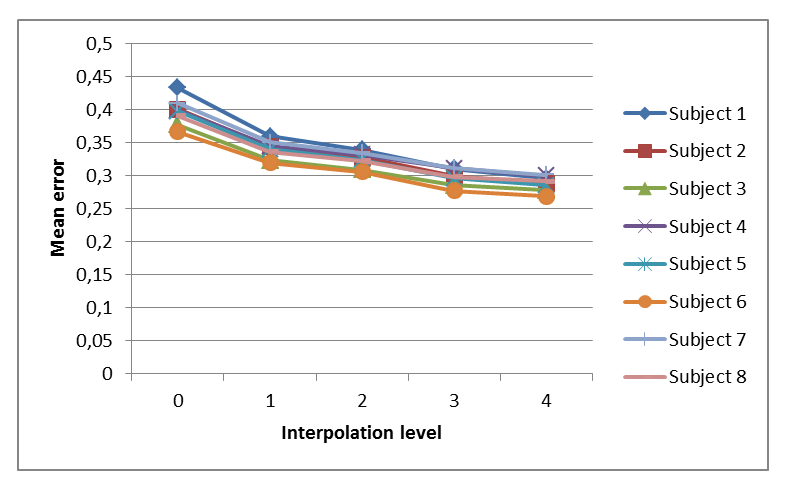
\epsfig{file = lh_whiteMatterInterpolationLevel.eps, width = 6cm}}
% \caption{Mean error for different start points of the log scale.}
% \label{fig:InterpolationLevel}
% \vspace{-0.1cm}
%\end{figure}

\section{Shape statistics of the cortex using CPNS}
\label{sec:Statistics}

%Statistics on objects has been applied to quite a variety of types of geometric model derived from the boundary
%cases:
%1. PCA has been applied to boundary point distribution models (\cite{cootes_training_1992}, \cite{kurtek_parameterization-invariant_2011}). 
%Kendall \cite{kendall_shape_2009} showed this is not correct as this type of models live in a space
%formed by a Cartesian product of a Euclidean space and high dimensional spheres. 
%Further developments yield a technique called PGA (principal geodesic analysis) \cite{angeles_generalized_2010} 
%which produced better statistics than PCA but still not satisfactory. 
%2.
%Deformation-of-atlas models, where the displacement of each voxel in the atlas
%is provided \cite{pennec_statistical_2009}, \cite{arsigny_log-euclidean_2006}). These models have enormous dimension, 
%and the statistical analysis is expensive and unstable with respect to the sampling
%into training cases and to noise in those training cases.
%3.
%Implicit models, such as level surfaces of pseudo-signed-distance functions \cite{clark_automatic_1998},
%that do not live in Euclidean feature spaces but are often analyzed (by PCA) as if they did.
%4.
%Skeletal models such as s-reps, live in abstract manifolds that are curved, 
%composed by a Cartesian product of a Euclidean space and a collection of spherical spaces.
%This type of models have many advantages as they capture information of the surface
%and the interior of the object by providing a local frame and a coordinate system
%created from the atoms sampled on the medial sheet. 
S-reps live in abstract manifolds that are curved,
composed by a Cartesian product of a Euclidean space and a collection of spherical spaces.
Using s-reps to compute shape statistics should yield better shape descriptors as volumetric information
is included into the analysis. 
Previous studies on s-reps of hippocampi have shown 
CPNS to yield lower-dimensional shape space with an efficient collection of modes of variation better than 
PCA-based statistical analysis of other skeletal or non skeletal models \cite{pizer_nested_2012}, \cite{schulz_2012}.
The analysis on the cortex is challenging since its dimension is very high and shape variations could go undetected
by the approach.

\begin{figure}[tb]
  \centering
  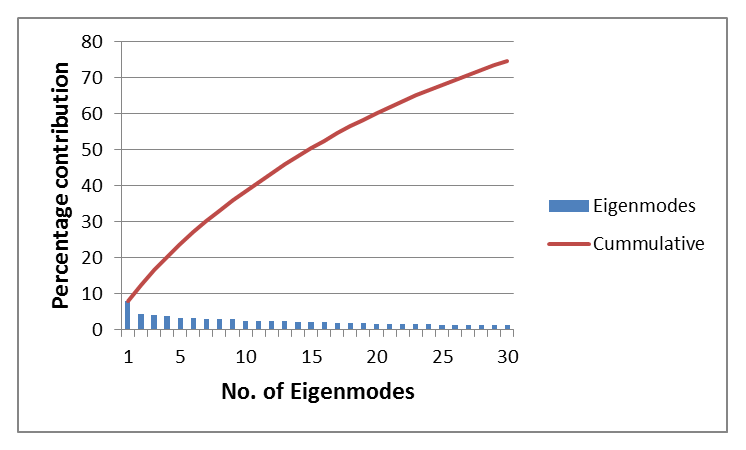
\epsfig{file = lh_CPNS_Eigen30.eps, width = 8cm}    
  \caption[Mean modes of variation for the cortex.]{Mean modes of variation for the cortical representation.}
  \label{fig:Modes}   
\end{figure}


The objective of using CPNS on the cortex is to detect cortical thickness variations.
In order to do this a test case is made using a base s-rep and 60 models derived from the same one.
The cortical thickness is reduced in specific regions of the cortex.
The datasets are created by adding some Gaussian noise to the position of the model, and to every spoke direction and radii in the s-rep. 
Each sample is going to be further modified with a linear variation of the cortical thickness,
specifically on the superior frontal and superior temporal regions of the cortex.
Spoke lengths are reduced $30\%$ of their original length.
If CPNS produces modes of variation, then the first mode should be related to the cortical thickness reduction.

Figure \ref{fig:Modes} shows the plot of the eigenvalues describing the mean modes of variation computed with CPNS.
The first mode is responsible for the largest variation found in the dataset and should correspond to 
thickness reduction in the specific areas. 

Figure \ref{fig:EigenVariation} shows the evolution of the model by manipulating the first mode of
variation. In the figure, the regions of the superior frontal
and superior temporal of the cortex are thinner, and adjacent structures remain constant through the deformation.
This can also be verified by checking the average thickness as shown in figure \ref{fig:thickness}.
As expected the first mode corresponds to the cortical thickness variation.

\begin{figure*}  
  \centering
  \subfigure[$+1.5 \sqrt{\lambda_1}$]{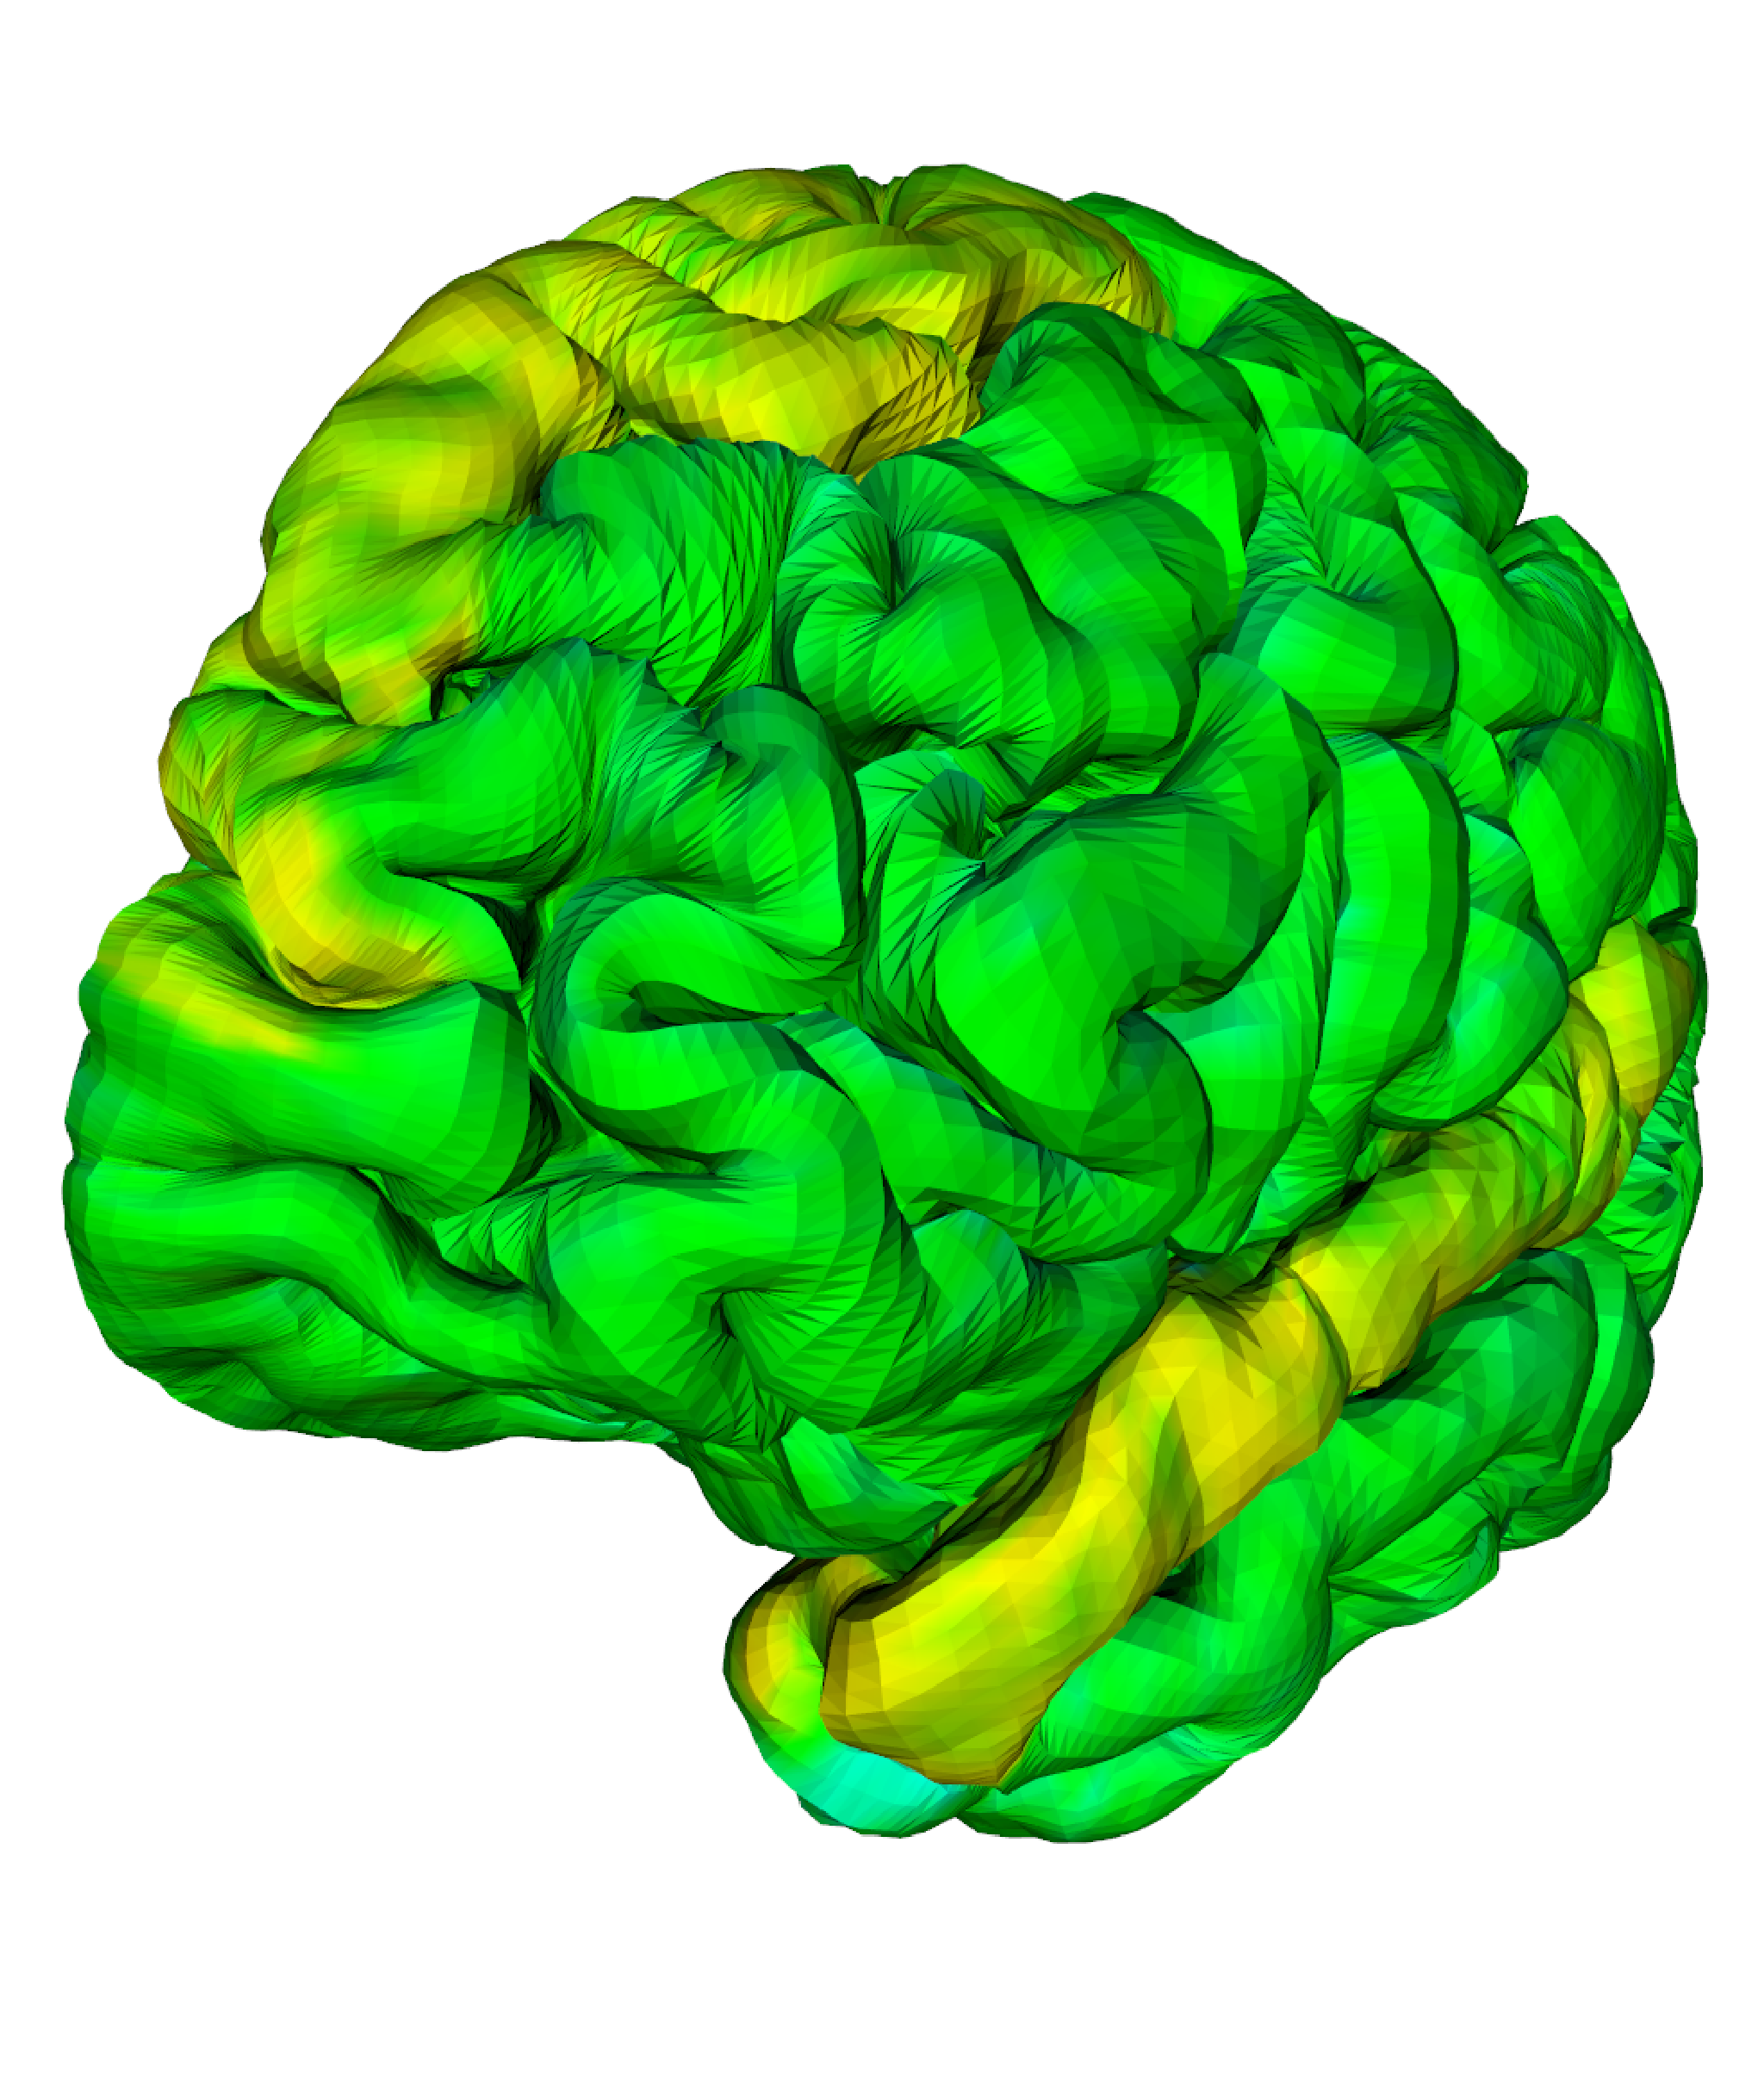
\epsfig{file = lh_EigenVariation30+1.5.eps, width = 3.5cm}}
  \subfigure[$+1  \sqrt{\lambda_1}$]{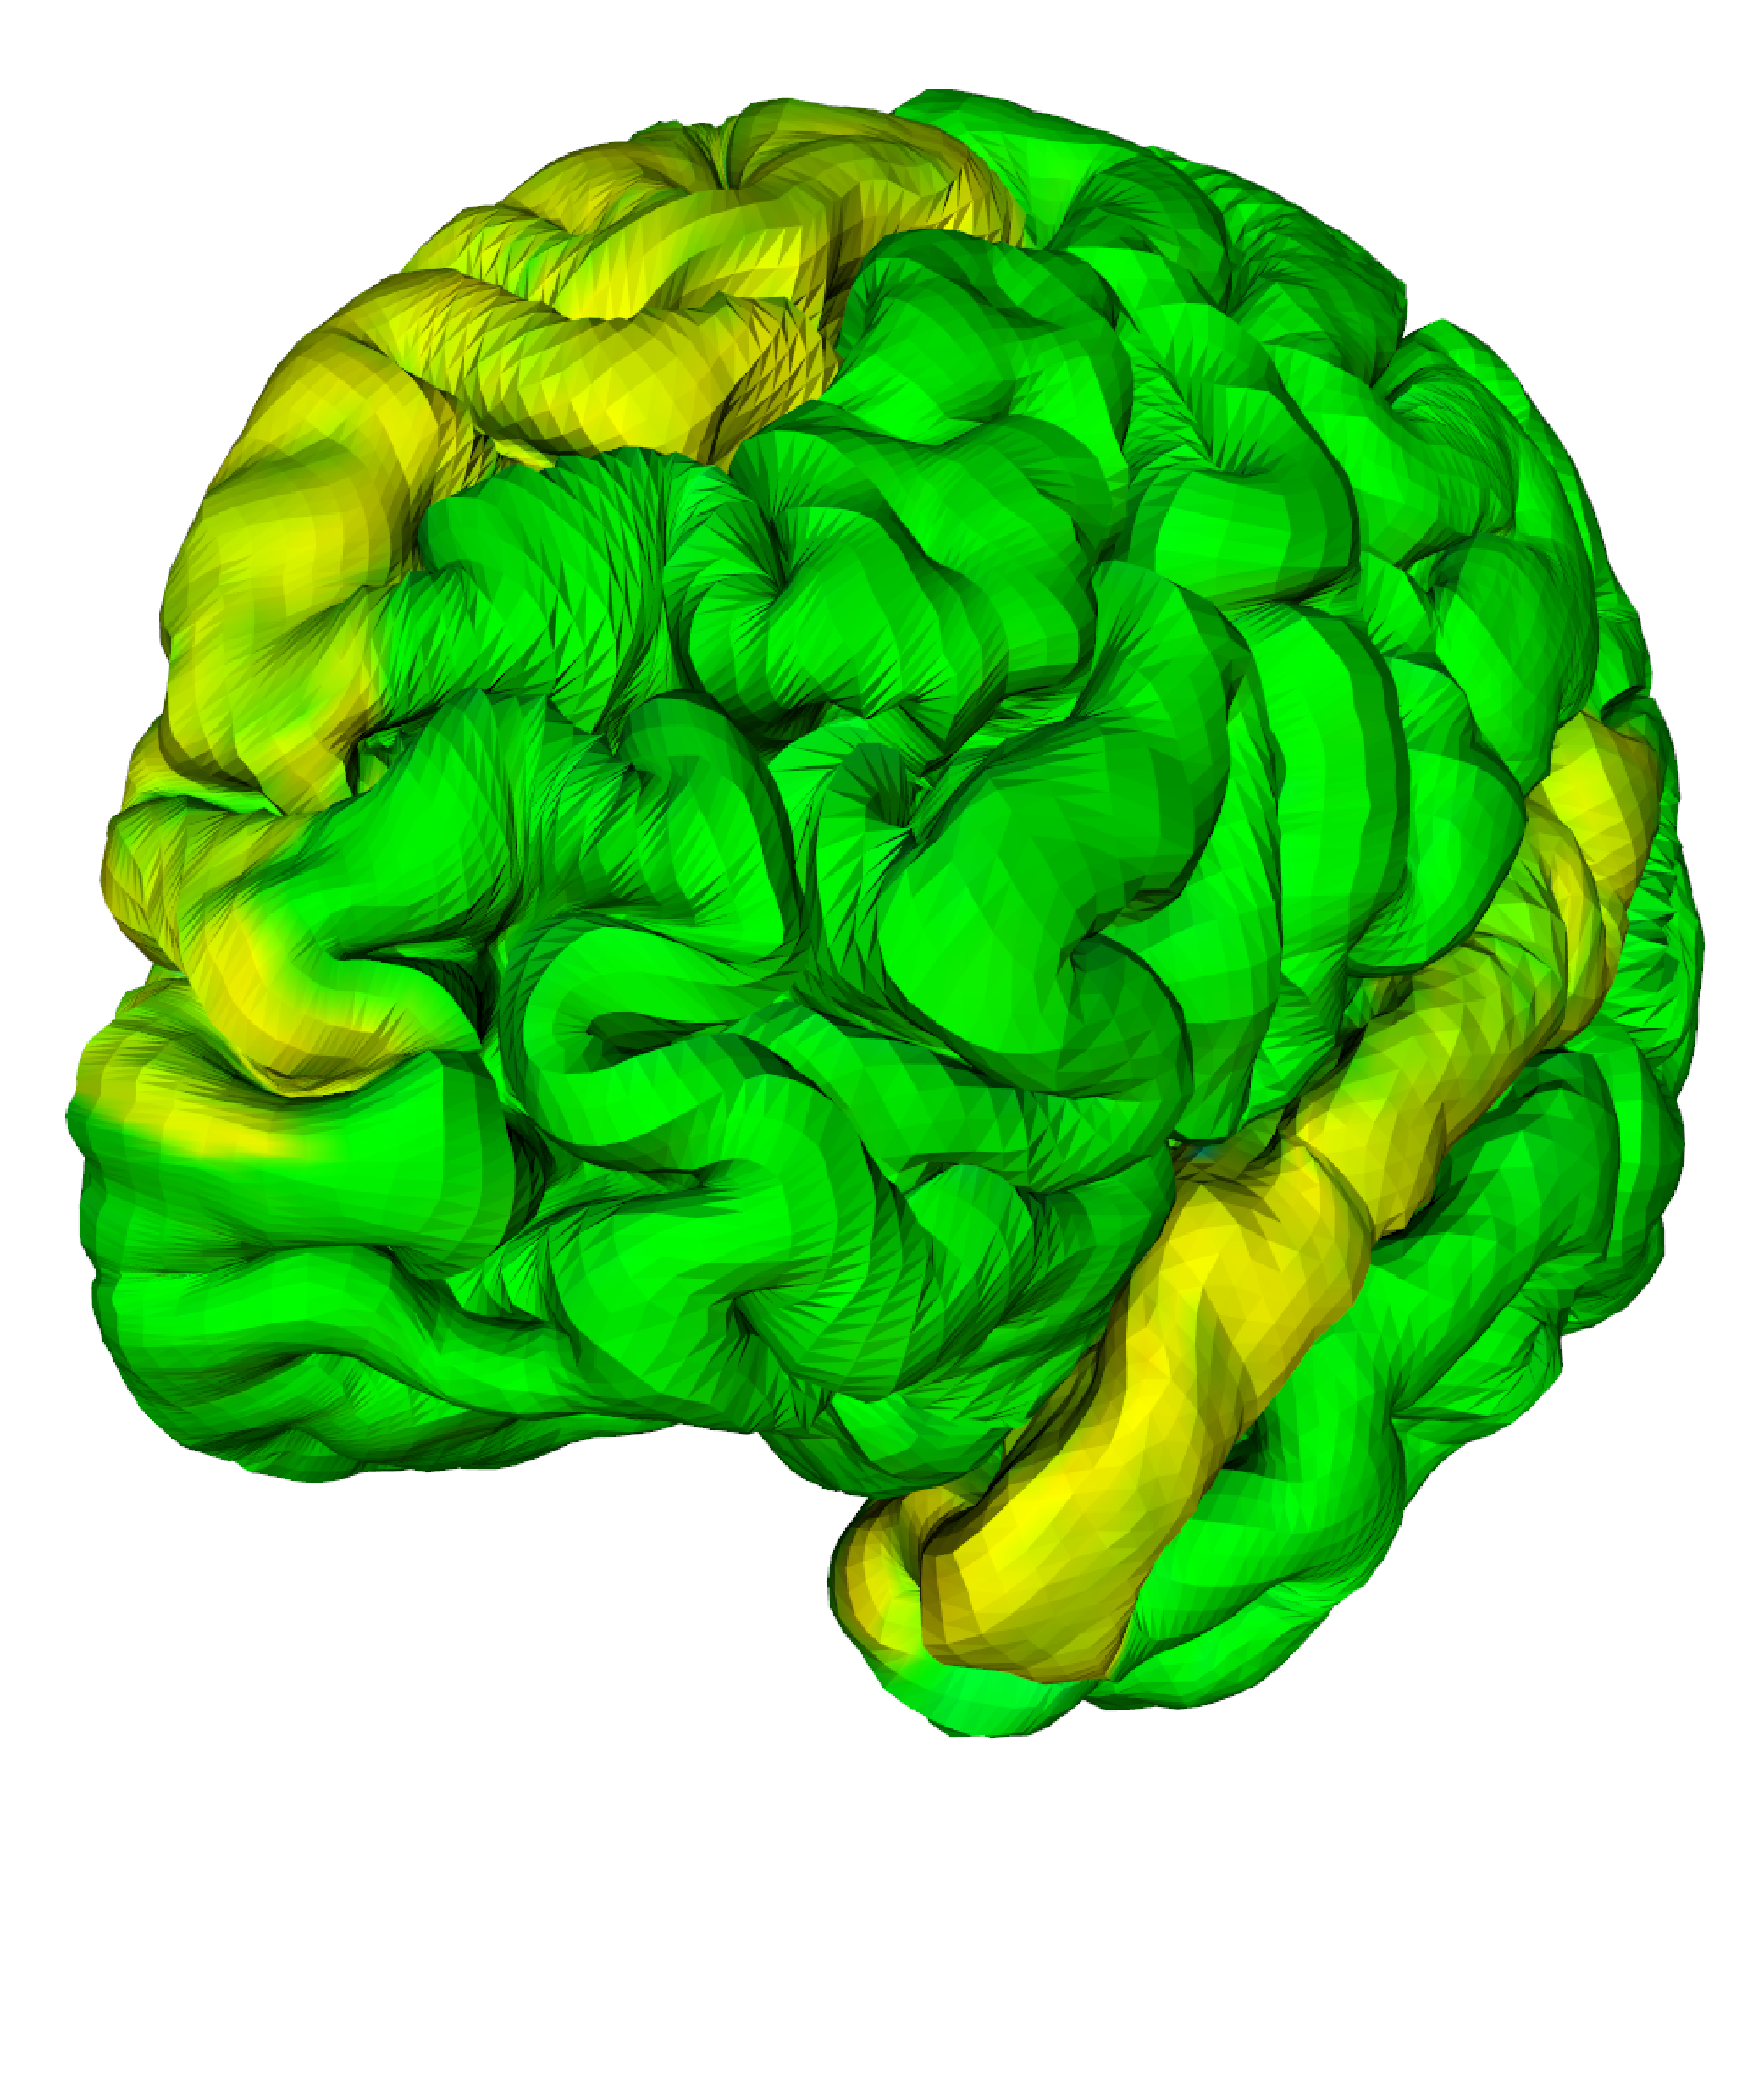
\epsfig{file = lh_EigenVariation30+1.eps, width = 3.5cm}}
  \subfigure[$+0.5 \sqrt{\lambda_1}$]{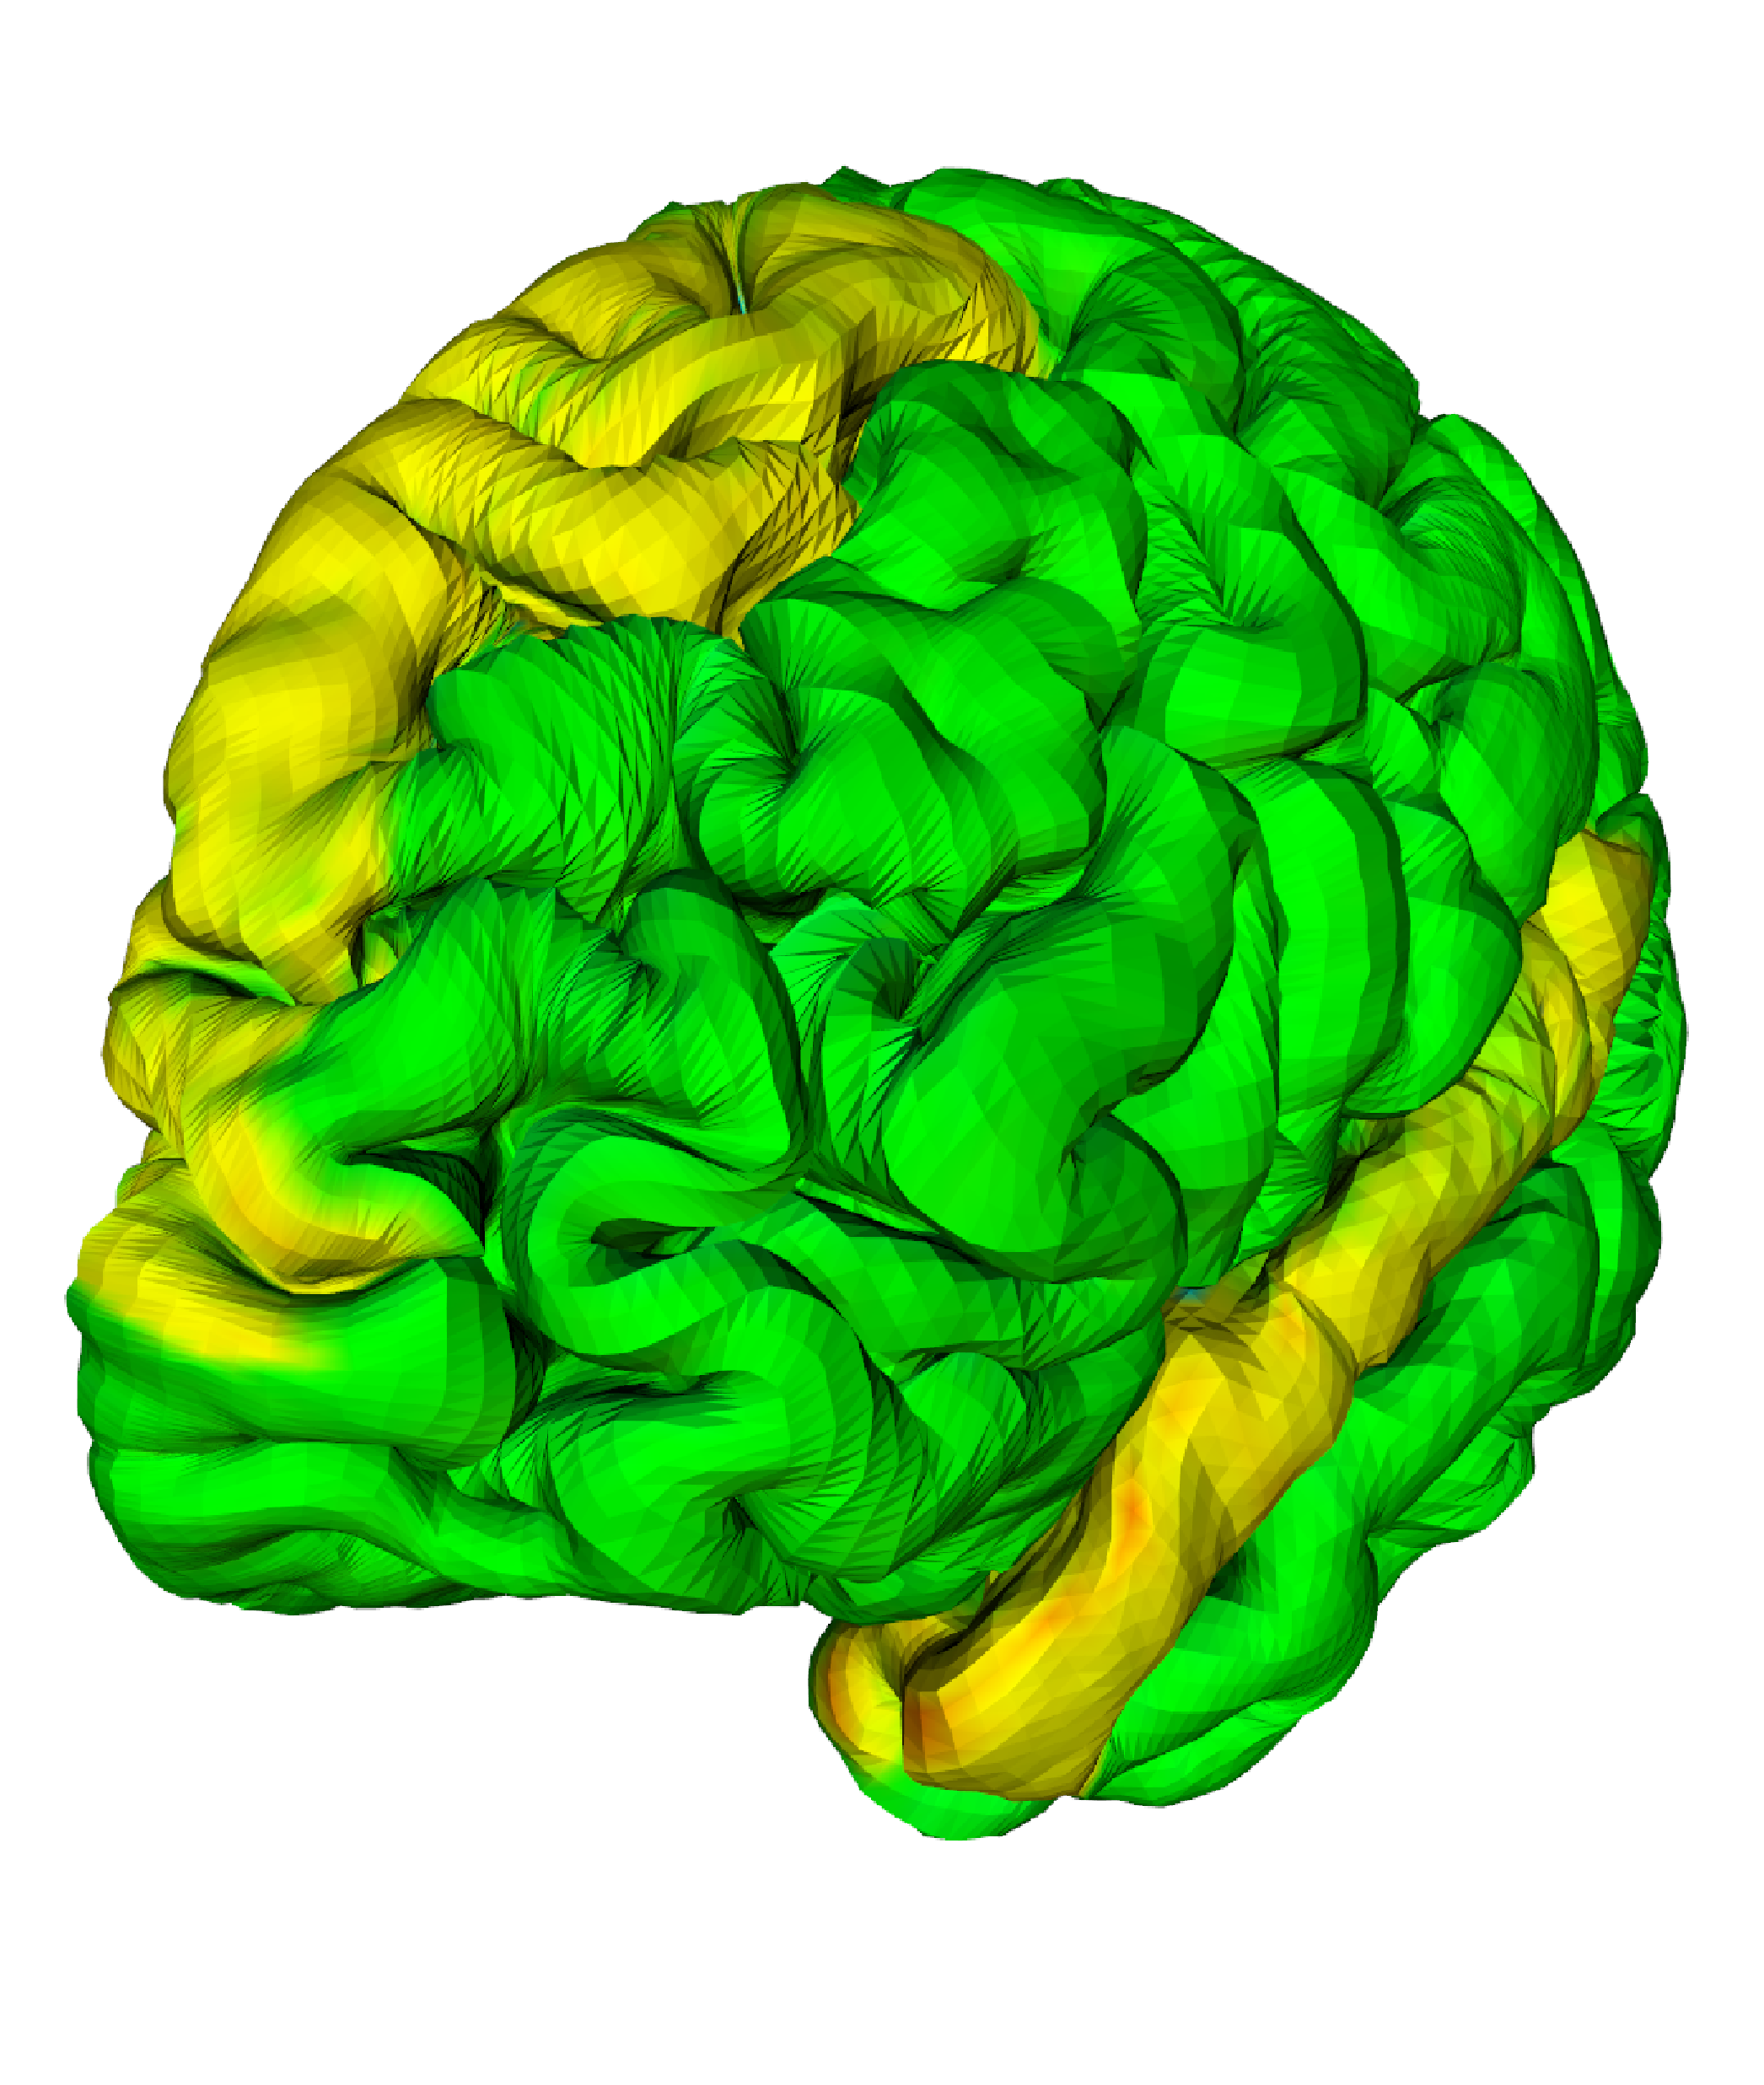
\epsfig{file = lh_EigenVariation30+0.5.eps, width = 3.5cm}}
  \subfigure[Mean]{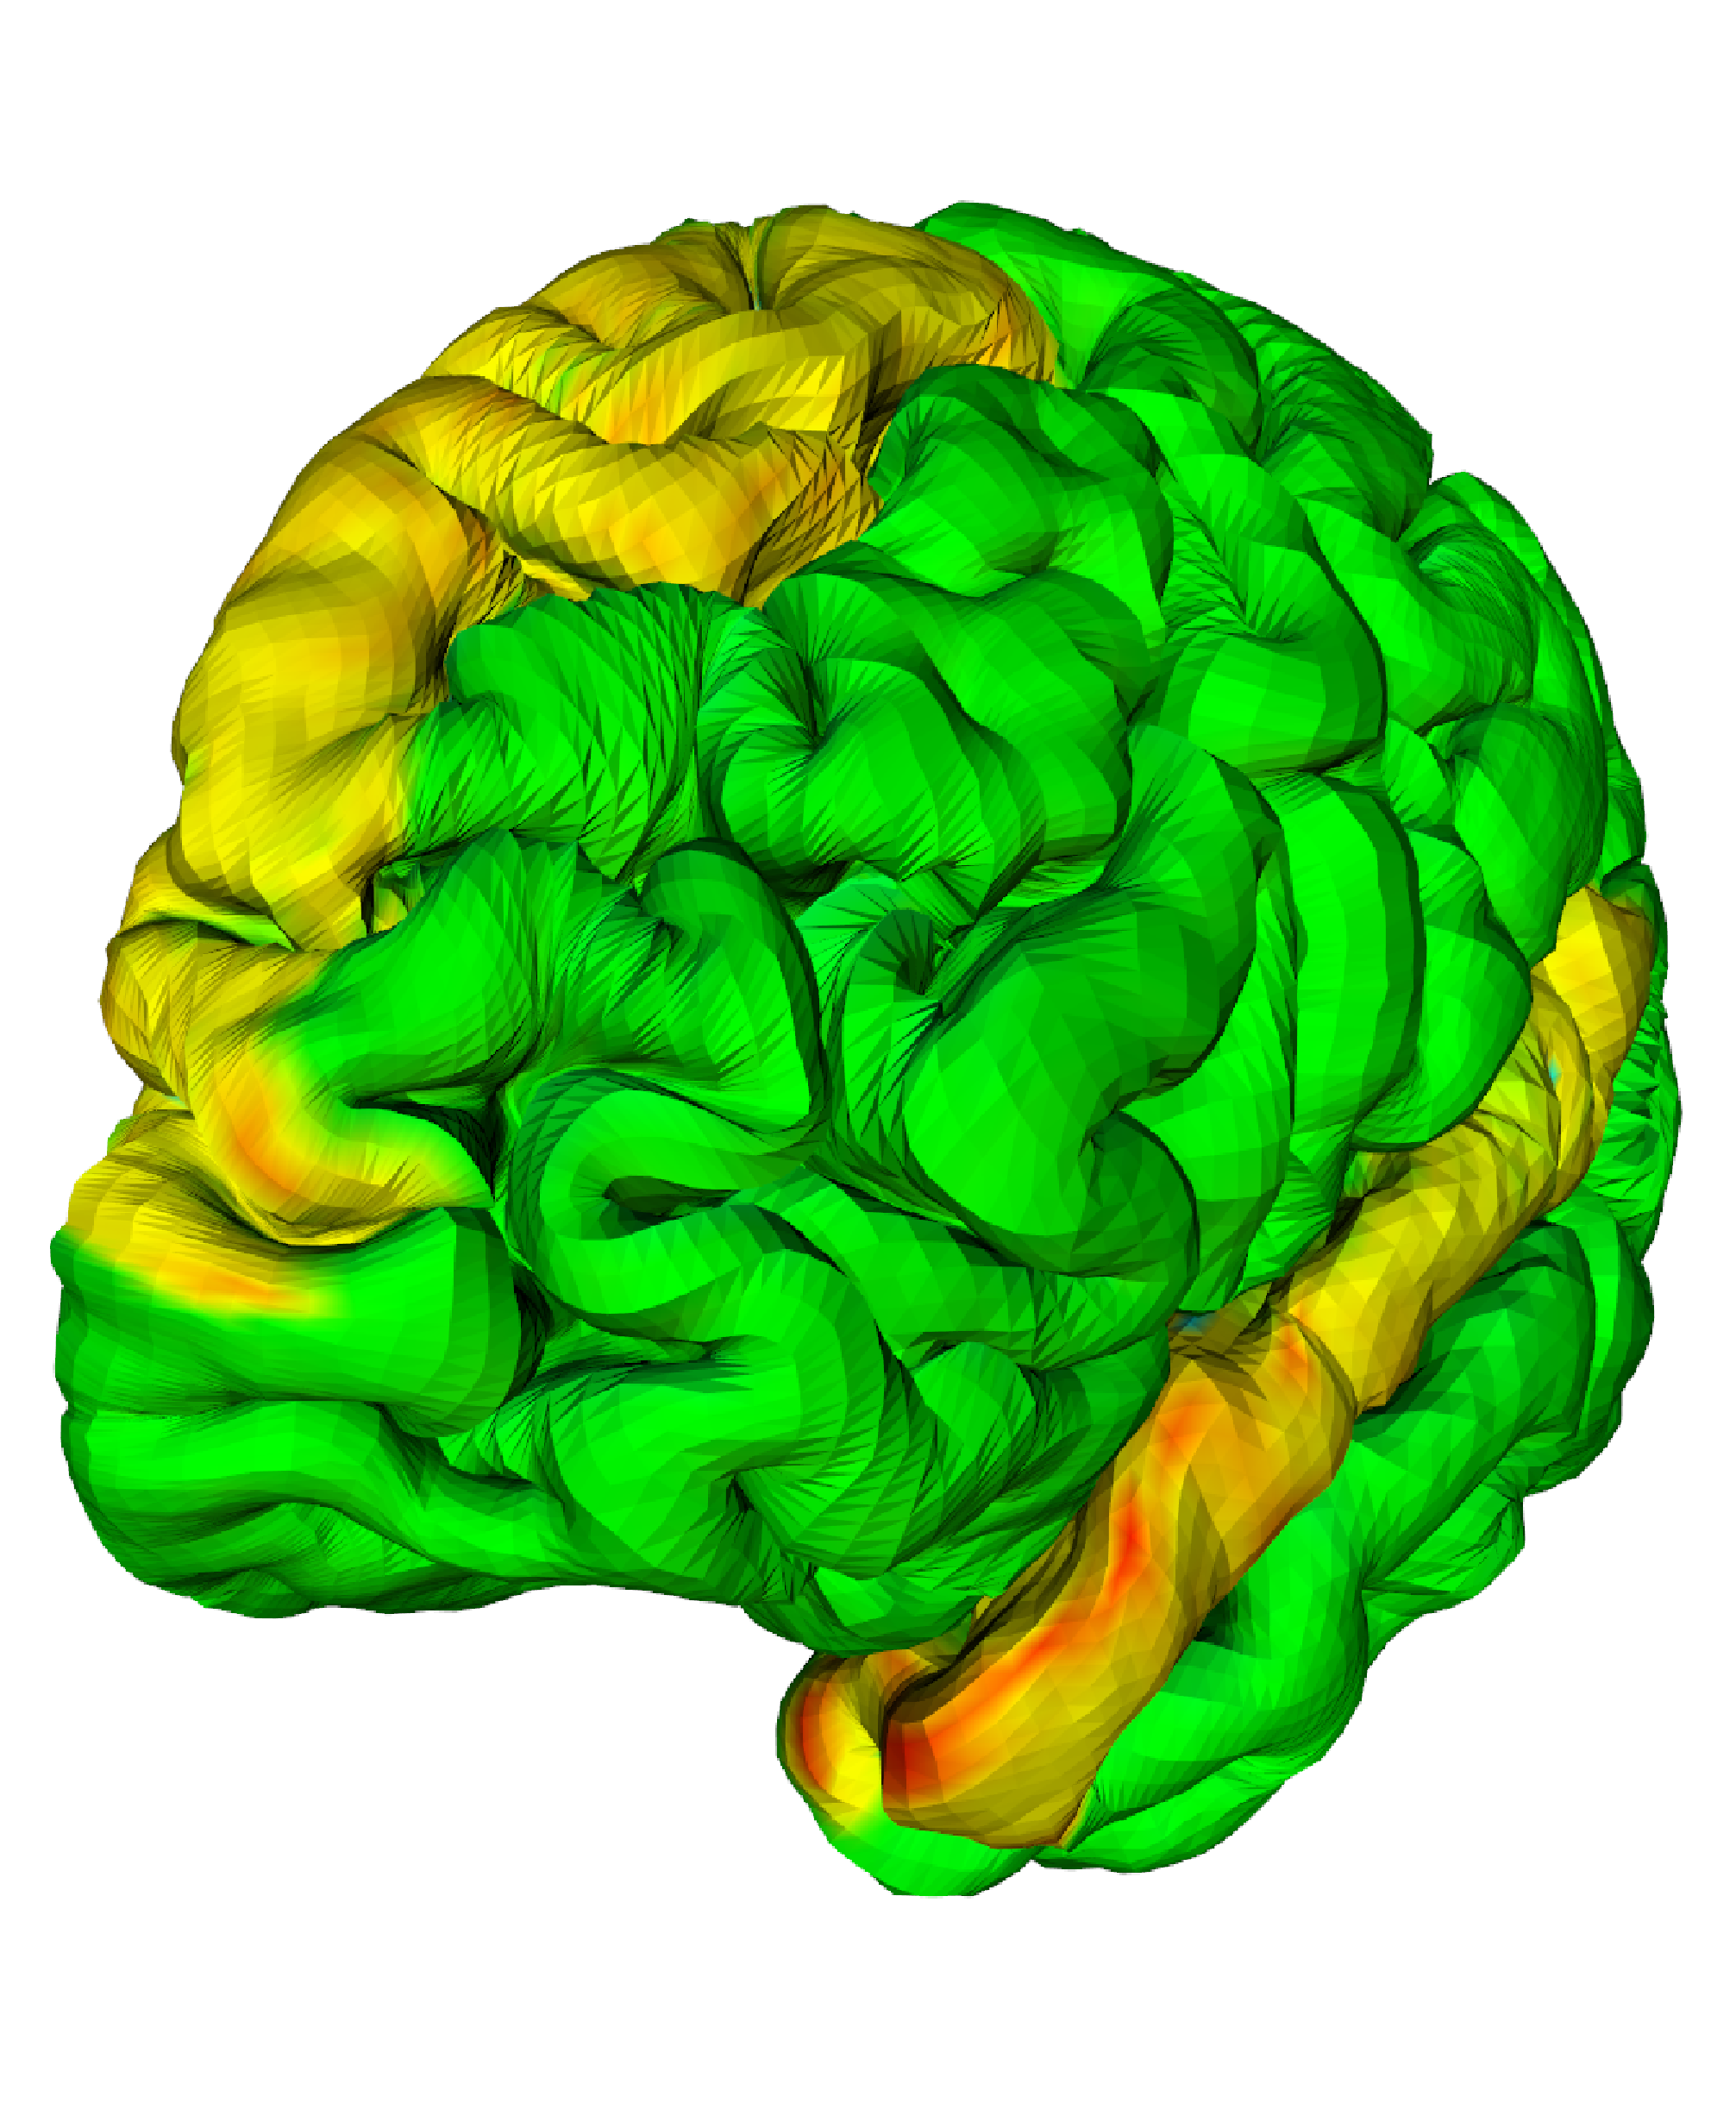
\epsfig{file = lh_EigenVariation30+0.eps, width = 3.5cm}}
  \subfigure[$-0.5 \sqrt{\lambda_1}$]{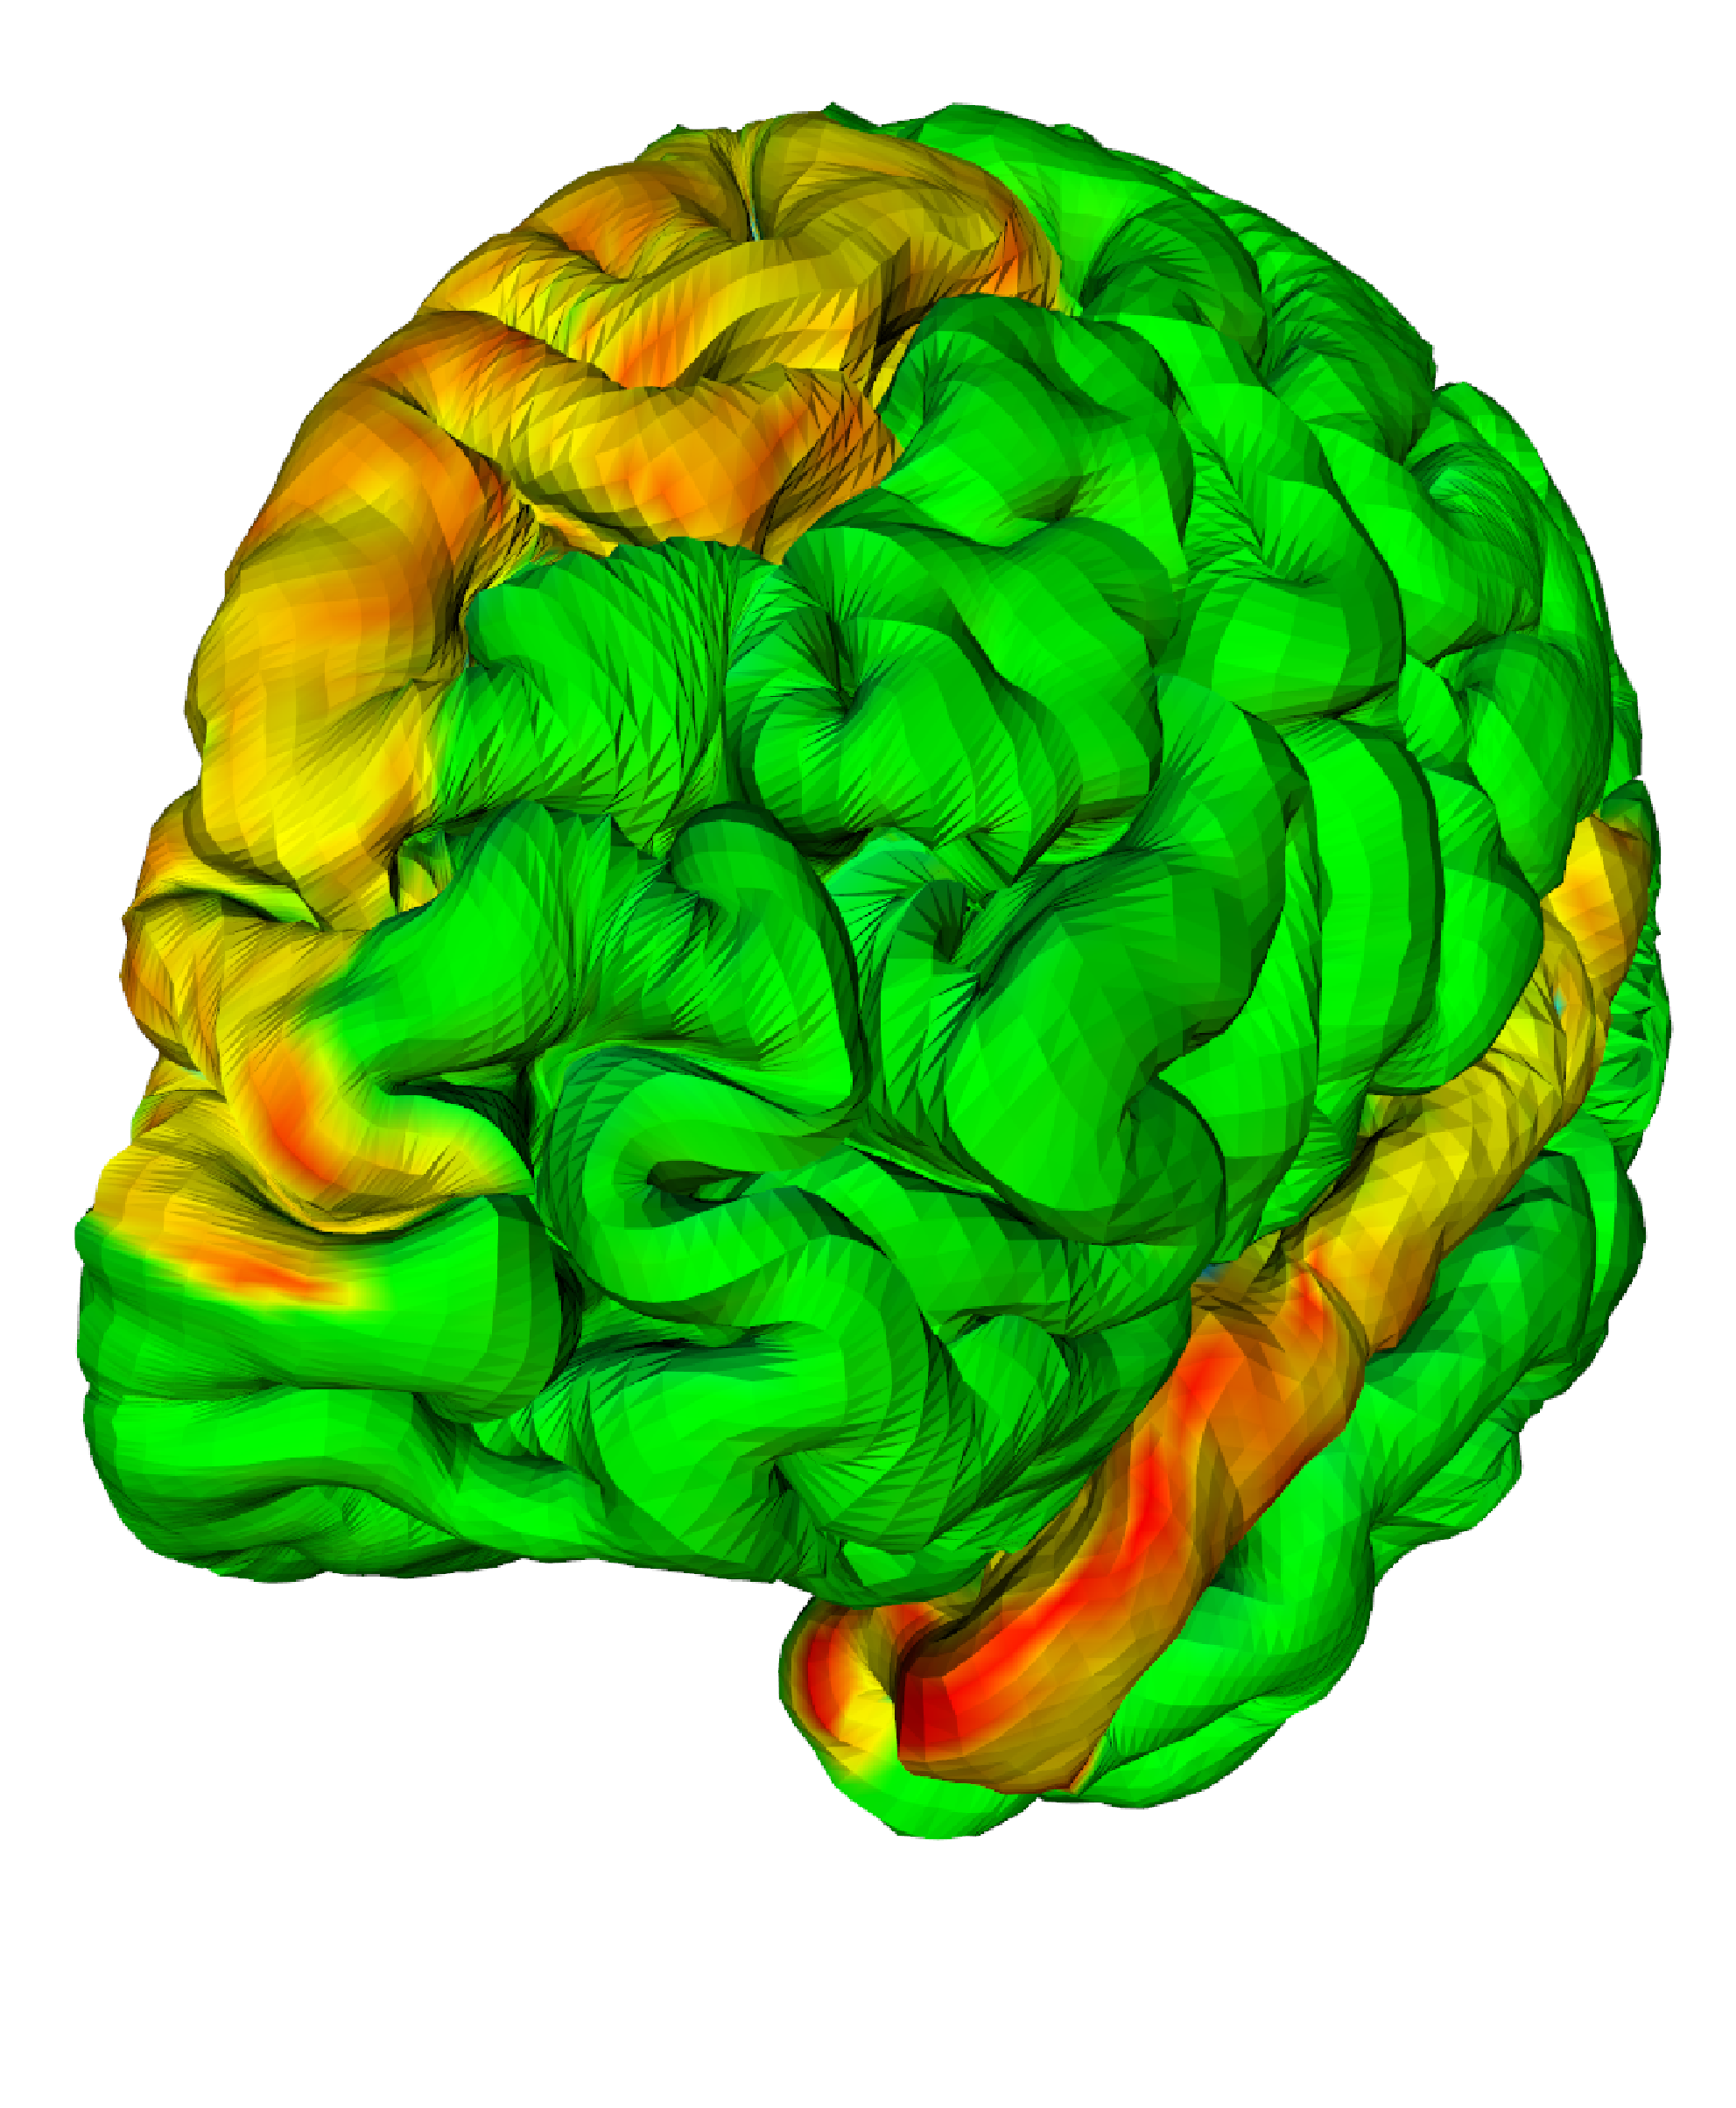
\epsfig{file = lh_EigenVariation30-0.5.eps, width = 3.5cm}}
  \subfigure[$-1 \sqrt{\lambda_1}$]{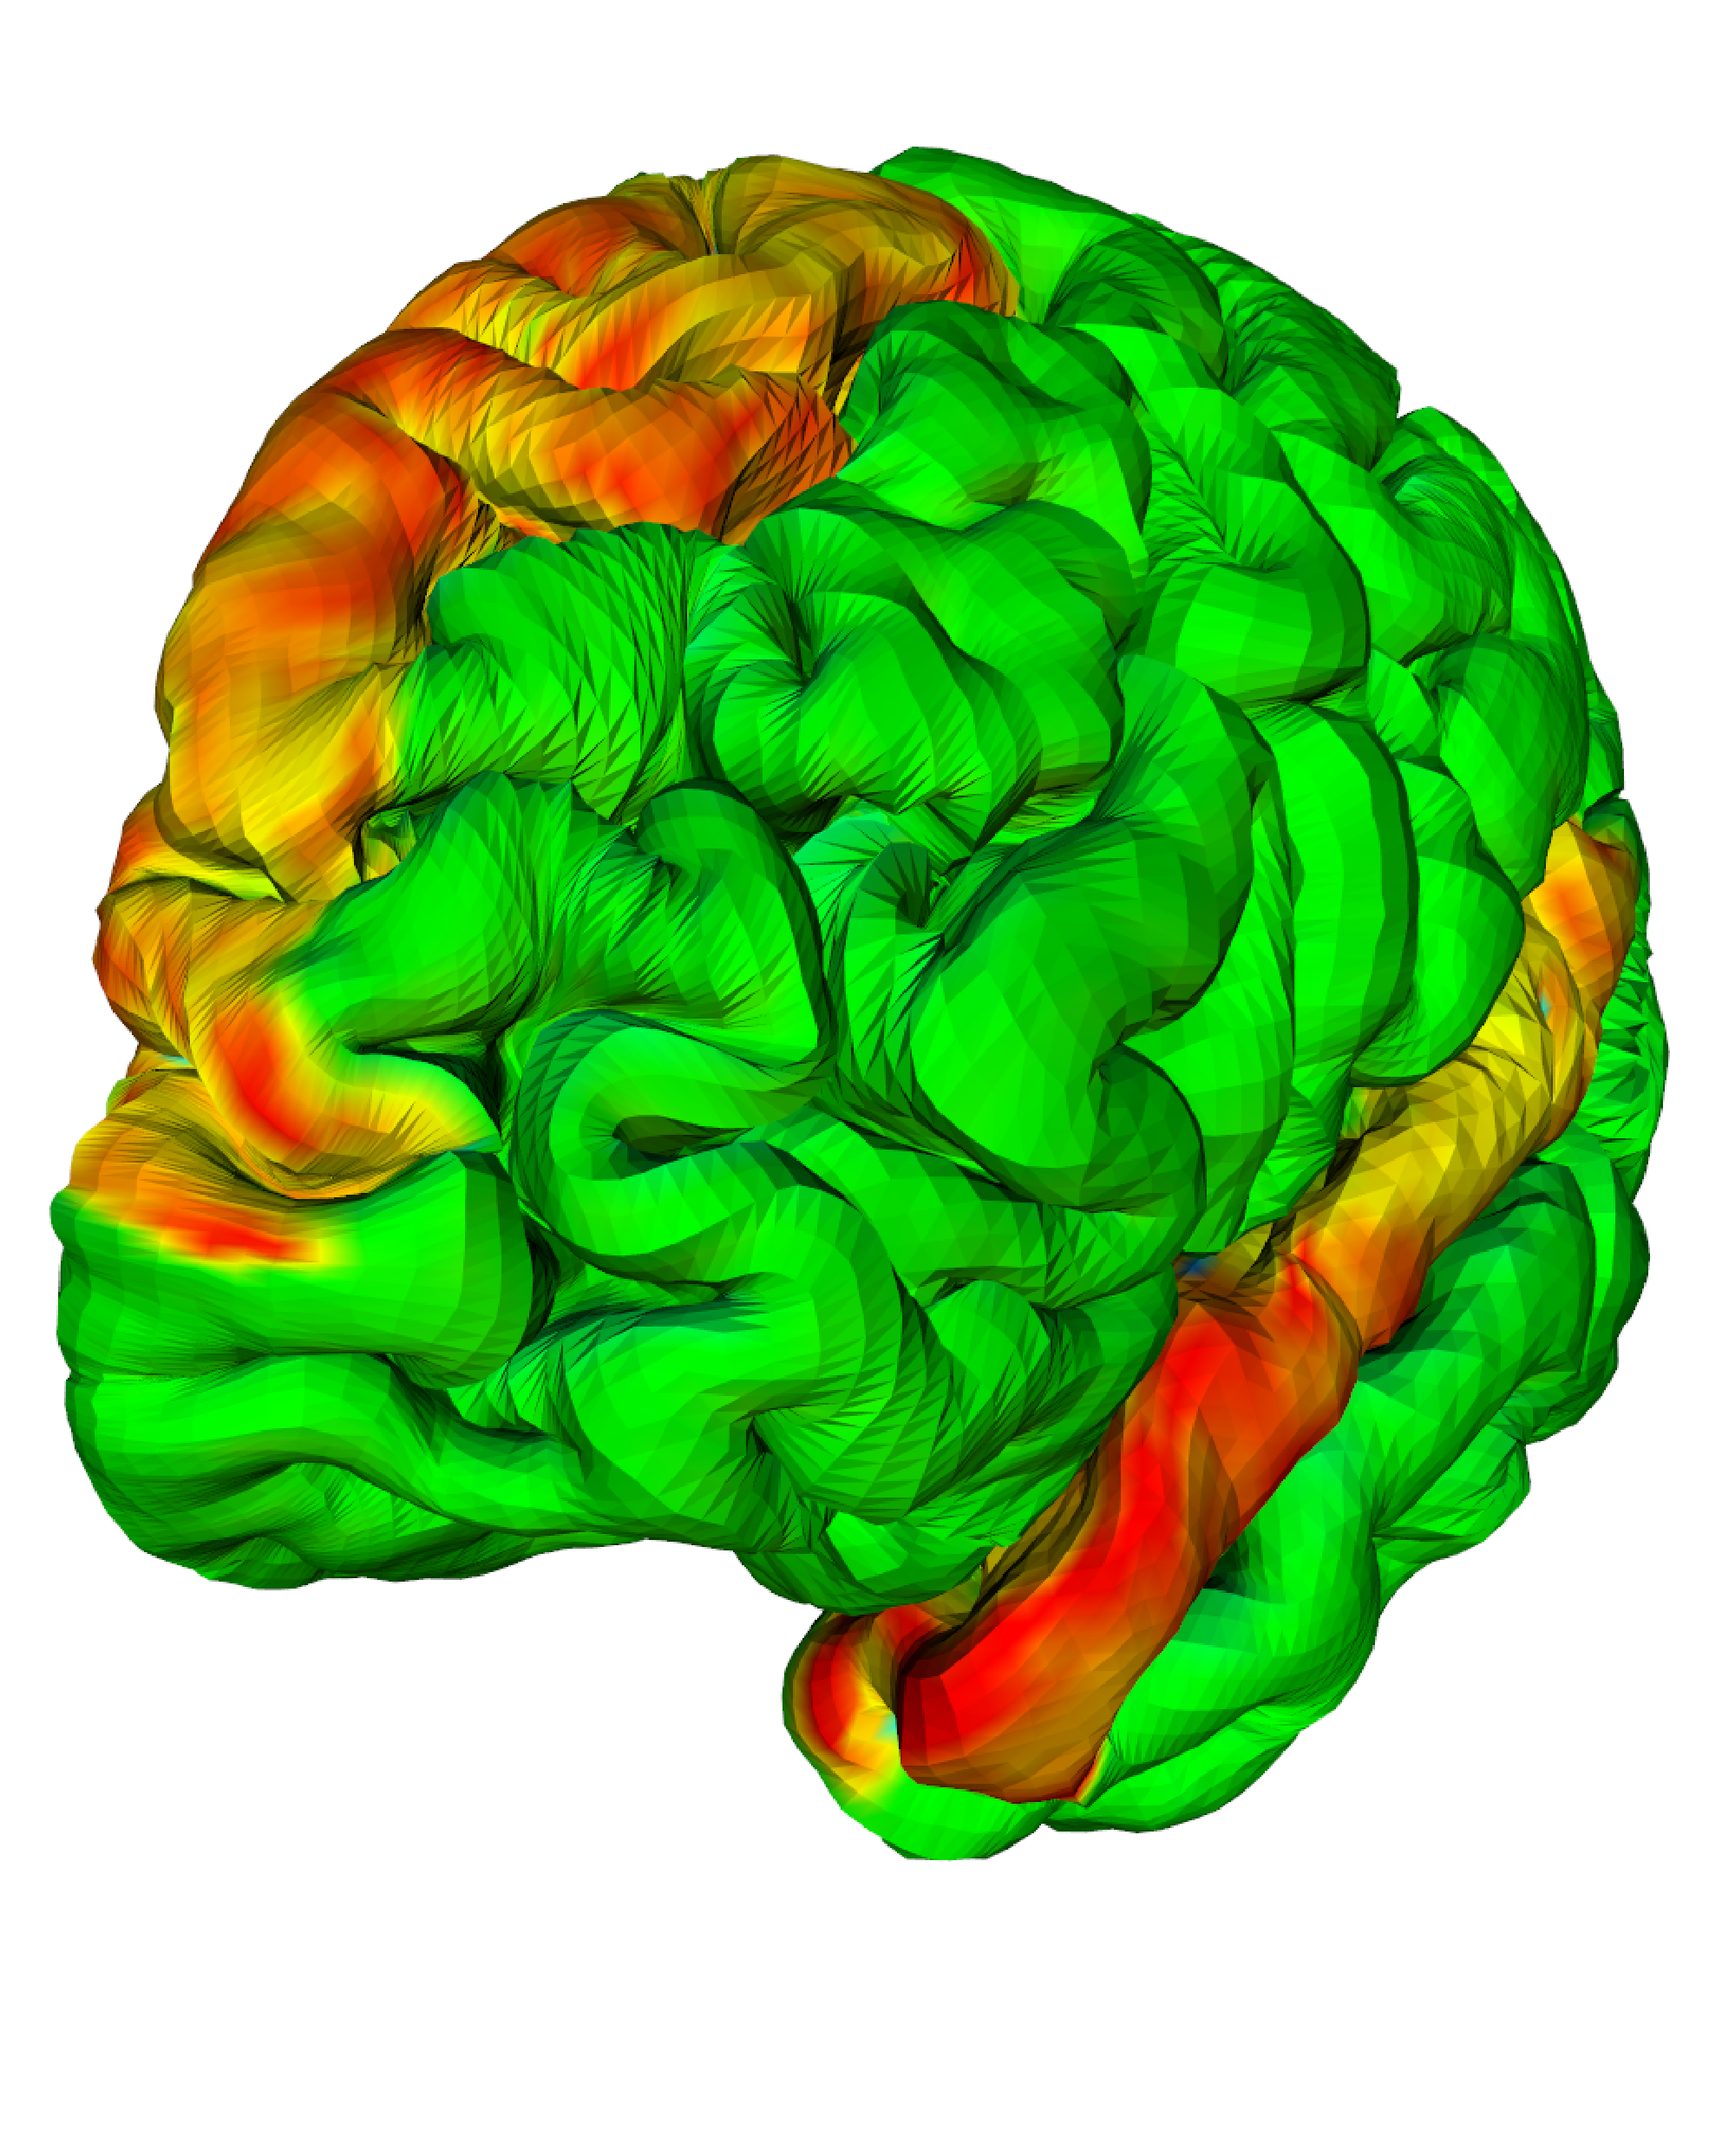
\epsfig{file = lh_EigenVariation30-1.eps, width = 3.5cm}}
  \subfigure[$+1.5 \sqrt{\lambda_1}$]{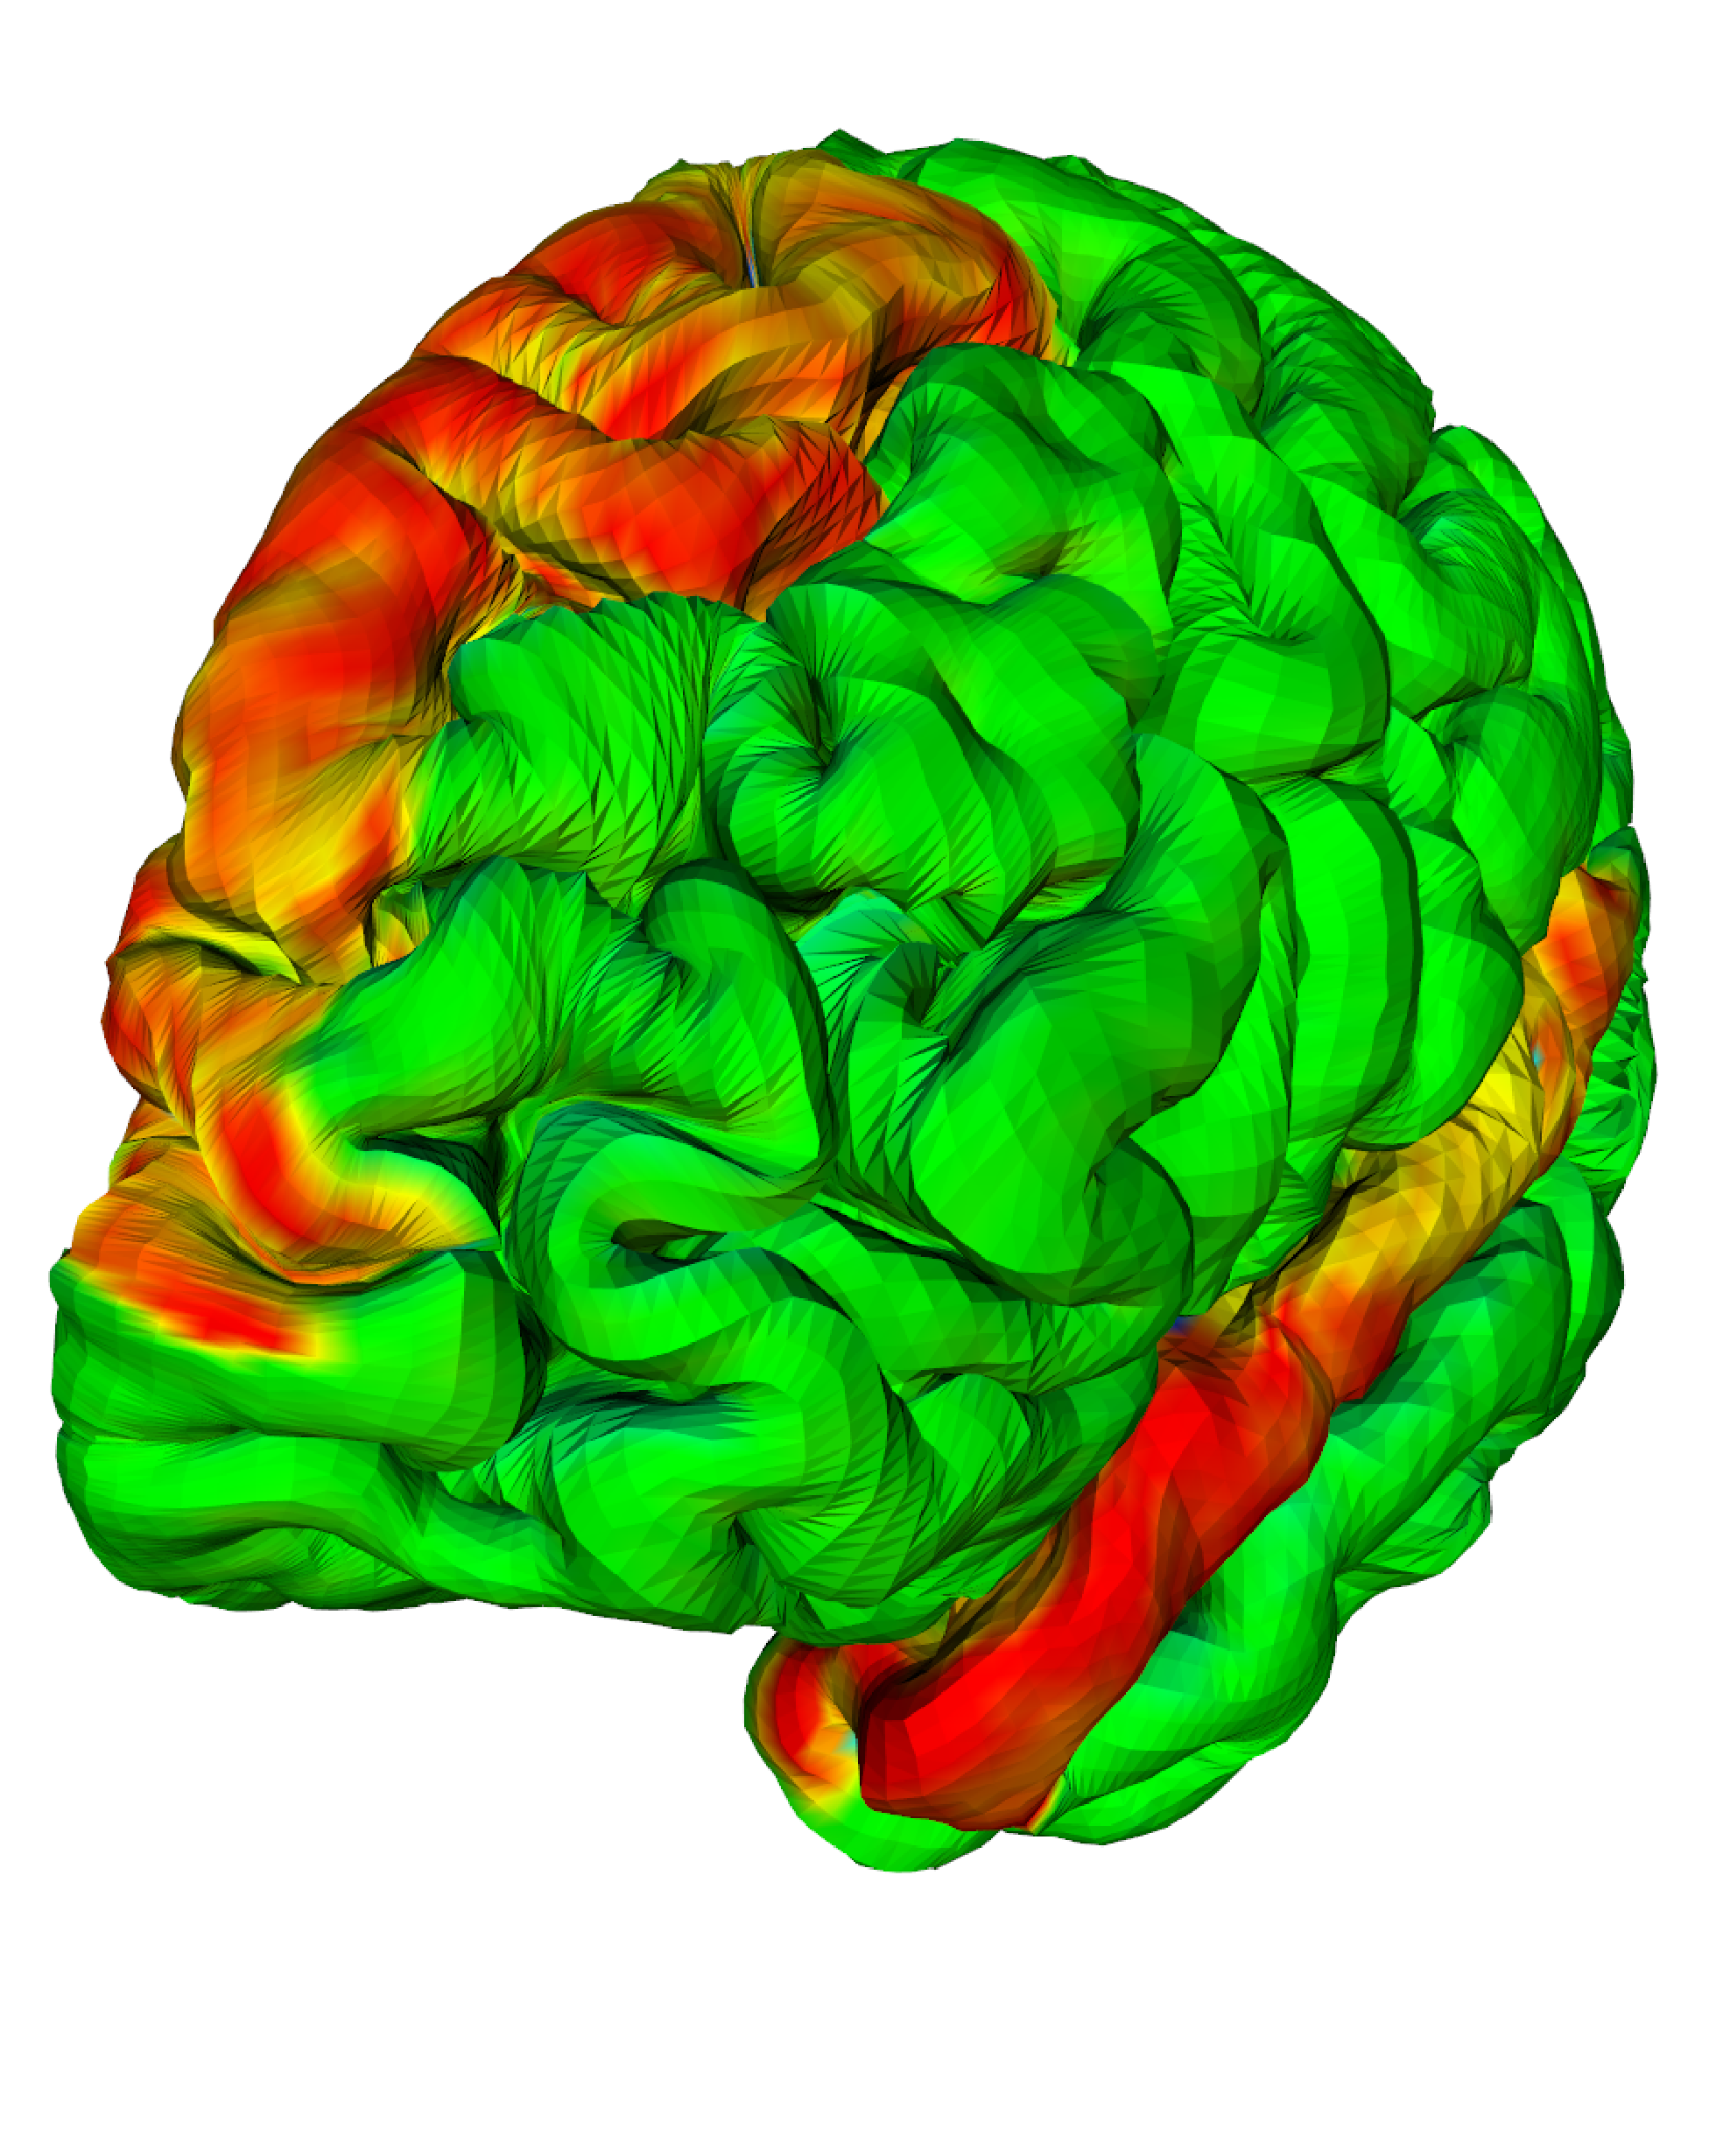
\epsfig{file = lh_EigenVariation30-1.5.eps, width = 3.5cm}}
  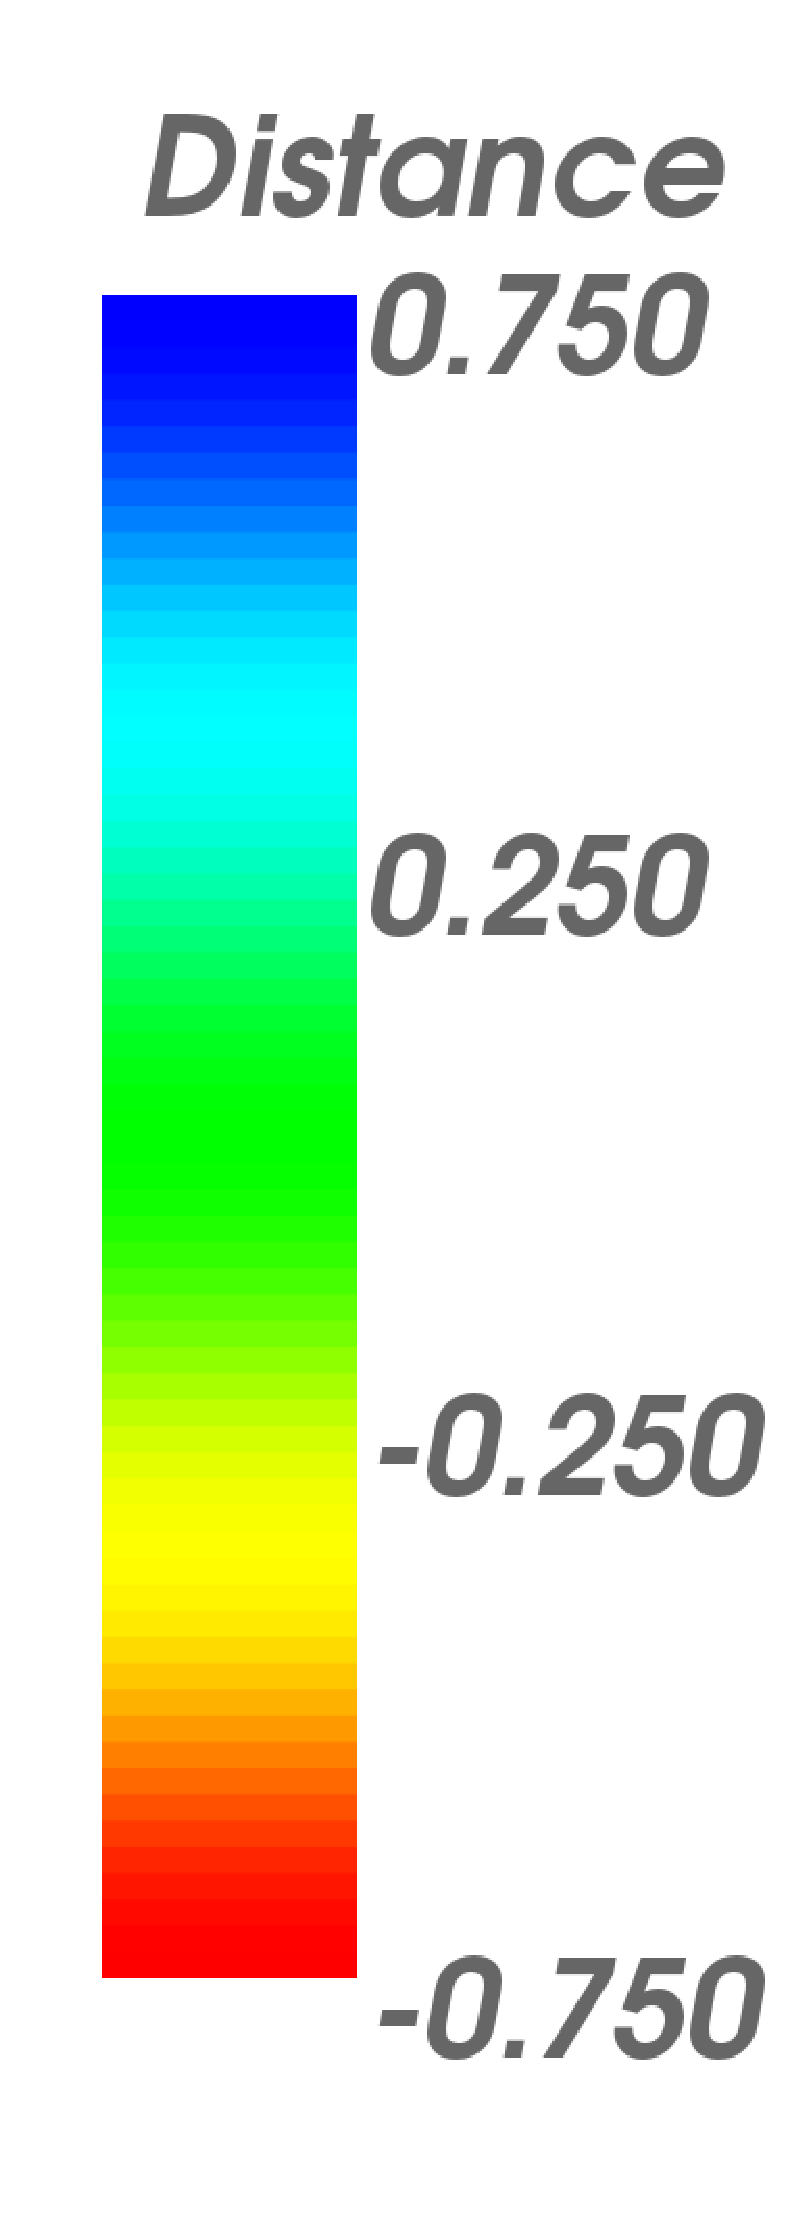
\epsfig{file = lh_EigenVariation30Bar.eps, width = 1.75cm}
  \caption[S-rep deformation using the first mode.]{Deforming the s-rep model using the first mode of variation and comparing it against the base s-rep.}
  \label{fig:EigenVariation}   
\end{figure*}

\begin{figure}[htb] 
  \centering
  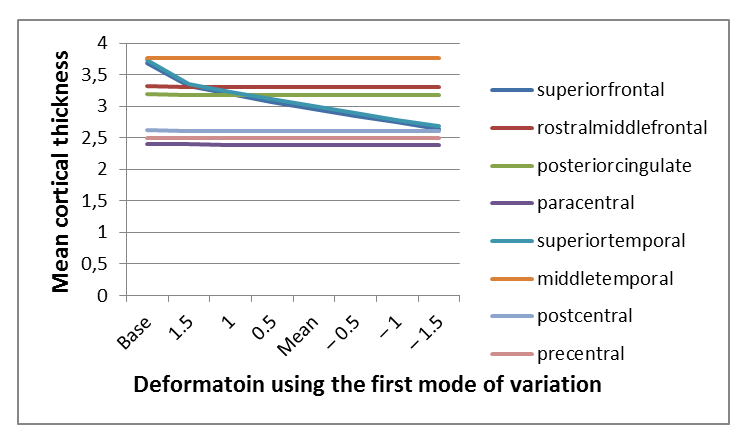
\epsfig{file = lh_EigenVariation.eps, width = 9cm}    
  \caption[Average thickness of the cortex.]{Average thickness for some cortical regions in the cortex. The two regions changing through the deformation
           are the superiorfrontal and superiortemporal.}
  \label{fig:thickness}   
\end{figure}


\section{Conclusion}
\label{sec:Conclusion}

One of the major contributions of this work is to represent the cortex as a folded slab using s-reps. 
S-reps are able to model continuum space. This characteristic can be used 
for the following purposes:
to include information in the cortex at different scale levels; provide 
new ways to analyze cortical columns, the building blocks of the cortical tissue;
analyze cortical lesions in a different space. 

These new advantages will use the local coordinate system $[u,v,\tau]$ provided by s-reps. 

A second contribution is to provide a compact representation of the cortex using CPNS. 
This statistical description models cortical thickness variations with a mean shape, some eigenmodes and a few coefficients.
Previous work with CPNS was done to study shape variations on the hippocampus using a grid size of $8*3$ atoms 
to represent the population of objects.
In this case, the s-rep size is $160 \times 160 $ atoms; nevertheless, CPNS was able to capture the localized thickness variation produced 
in the superior-frontal and superior-temporal regions of the cortex. 
This suggests that the approach could
produce statistics for longitudinal clinical 
cases that are characterized by cortical thickness variations. 
Cortical thinning is a natural process of aging \cite{doi:10.1080/13803390802635174}.
Other clinical cases such as psychosis, schizophrenia, hyperactivity disorder in children and autism
also present abnormal cortical thickness variations.

A third contribution is to model the cortex of different patients using the same underlying skeletal structure.
A test case was done to compute a mean shape of the cortex for the 8 patients used in this study. 
%This characteristic could be exploited if the statisitcs are computed for a crosswise scenario.
%Any approach that computes shape statistics, must have 
%a stable set of points or landmarks across the population and this is achieved using the SS of the s-rep.
Figure \ref{fig:CPNSMean} shows the mean surface for the 8 datasets computed with \textit{Freesurfer} and
CPNS. 
%To compute CPNS with the 8 subjects used in this study, 
%the cortical regions mapped on the sphere 
%are aligned to a generic template. 
%Using the aligned spheres to generate the s-reps
%increases the correspondence of the SS accross the population. 
%Each hub of the s-rep should map to the same region 
%in the cortex in order to perform an accurate 
%statistical analysis of shape with CPNS. 

Unfortunately in this case, CPNS was not able to detect principal modes of variation.
%and yield the set of eigenmodes unusable.
This could be for two reasons. The main one is related to the number of datasets 
used in the study. The dimension of the s-rep 
is too high compared to the sample size.
The second reason could be related to the alignment 
of each of the cortical regions. 
To produce accurate shape statistics, the objects must be aligned correctly.


\begin{figure}  
  \centering
  \subfigure[CPNS mean]{\epsfig{file = cortexCompareCPNS.eps, width = 7.25cm}}
  \subfigure[\textit{Freesurfer} mean]{\epsfig{file = cortexCompareFreesurfer.eps, width = 7.25cm}}
  \subfigure[Overlap]{\epsfig{file = cortexCompareOverlap.eps, width = 8.5cm}}  
  \caption[Mean shape of the cortex: CPNS and \textit{Freesurfer}.]{Mean shape computed from the 8 datasets.}
  \label{fig:CPNSMean}   
\end{figure}

It has been proven that s-reps are suitable 
entities to model the complex shape of the cortex and provide new ways of cortex analysis. 

Future work considers the following possibilities:
the first opportunity is related to shape analysis of the cortex in 
multiple subjects scenarios. The objective is to produce a usable set of coefficients
and eigenmodes that models a population of cortices.
A second opportunity is related to cortex analysis on longitudinal scenarios. 
For this purpose three or more acquisitions of a patient at different time points could be used 
to study the process of aging. 

The work presented here showed that CPNS can detect cortical thinning on a set of cortices; 
a third line of work seeks to describe the folding procedure of the cerebral cortex
using shape descriptors.

The following chapter explains a texture synthesis technique to create volumetric representations using 
2D image samples. The volumes can be used on s-rep models to create 
solid objects.


\newpage

